\documentclass[aspectratio=169, 10pt]{beamer}

% =============================================================================
% PACKAGES & ENCODING
% =============================================================================
\usepackage[utf8]{inputenc}
\usepackage[T1]{fontenc}
\usepackage{helvet}
\renewcommand{\familydefault}{\sfdefault}
\usepackage{amsmath,amssymb}
\usepackage{graphicx}
\usepackage{booktabs}
\usepackage{tabularx}
\usepackage{colortbl}
\usepackage{xcolor}
\usepackage{tikz}
\usetikzlibrary{shapes,arrows,positioning,calc}
\usepackage[most]{tcolorbox}

% =============================================================================
% COLOR PALETTE (ACADEMIC BLUE THEME)
% =============================================================================
\definecolor{NavyDark}{HTML}{0F172A}     % Slate 900
\definecolor{BluePrimary}{HTML}{1D4ED8}  % Royal Blue 700
\definecolor{BlueLight}{HTML}{EFF6FF}    % Blue 50
\definecolor{BlueBorder}{HTML}{3B82F6}   % Blue 500
\definecolor{BlueDeep}{HTML}{1E3A8A}     % Blue 900
\definecolor{TextBody}{HTML}{1E293B}     % Slate 800
\definecolor{TextMuted}{HTML}{475569}    % Slate 600
\definecolor{CanvasBG}{HTML}{F8FAFC}     % Slate 50
\definecolor{CanvasBorder}{HTML}{CBD5E1} % Slate 300
\definecolor{GoldBG}{HTML}{FFFBEB}       % Amber 50
\definecolor{GoldBorder}{HTML}{EAB308}   % Amber 500
\definecolor{GoldPill}{HTML}{B45309}     % Amber 700

% =============================================================================
% BEAMER THEME & TEMPLATE CONFIGURATION
% =============================================================================
\setbeamercolor{background canvas}{bg=CanvasBG}
\setbeamercolor{normal text}{fg=TextBody}
\setbeamercolor{frametitle}{fg=NavyDark, bg=CanvasBG}
\setbeamercolor{title}{fg=NavyDark}
\setbeamercolor{subtitle}{fg=BluePrimary}
\setbeamerfont{frametitle}{size=\normalsize,series=\bfseries}
\setbeamerfont{framesubtitle}{size=\tiny,series=\normalfont}

\setbeamersize{text margin left=0.55cm, text margin right=0.55cm}
\setbeamertemplate{navigation symbols}{}

% Custom Frame Header
\setbeamertemplate{frametitle}{
  \vspace{0.10cm}
  \begin{beamercolorbox}[wd=\textwidth,leftskip=0cm,rightskip=0cm]{frametitle}
    {\color{BluePrimary}\tiny\bfseries\fboxsep=1.8pt\colorbox{BlueLight}{\insertframesubtitle}}\\[0.04cm]
    {\fontsize{11.5pt}{13pt}\selectfont\bfseries\color{NavyDark}\insertframetitle}
  \end{beamercolorbox}
  \vspace{-0.40cm}
}

% Custom Frame Footer
\setbeamertemplate{footline}{
  \begin{beamercolorbox}[wd=\paperwidth,ht=0.35cm,dp=0.15cm,leftskip=0.55cm,rightskip=0.55cm]{footline}
    \tiny\color{TextMuted}
    MNIT Jaipur $\bullet$ Dept. of CSE \hfill
    \textbf{AcuLearn AI} $\bullet$ Pre-PhD Open Seminar $\bullet$ 19 November 2026 \hfill
    \textbf{Slide \insertframenumber{} of \inserttotalframenumber}
  \end{beamercolorbox}
}

% =============================================================================
% CUSTOM TCOLORBOX CONTAINERS (LARGE FONTS & EXPANDED VISUAL FRAMES)
% =============================================================================
\newtcolorbox{defensecard}[1]{
  colback=white,
  colframe=BlueBorder,
  arc=1.8mm,
  boxrule=0.9pt,
  coltitle=NavyDark,
  fonttitle=\small\bfseries,
  title={#1},
  colbacktitle=BlueLight,
  toptitle=0.8mm,
  bottomtitle=0.8mm,
  top=1.2mm,
  bottom=1.2mm,
  left=2.8mm,
  right=2.8mm,
  boxsep=0.4mm
}

\newtcolorbox{topsummarybar}{
  colback=BlueLight,
  colframe=BlueBorder,
  arc=1.5mm,
  boxrule=0.8pt,
  top=1.0mm,
  bottom=1.0mm,
  left=2.8mm,
  right=2.8mm,
  boxsep=0.3mm
}

\newtcolorbox{diagramframe}{
  colback=white,
  colframe=BlueBorder,
  arc=1.5mm,
  boxrule=0.8pt,
  halign=center,
  valign=center,
  top=0.3mm,
  bottom=0.3mm,
  left=0.3mm,
  right=0.3mm
}

\newtcolorbox{takeawaybanner}{
  colback=GoldBG,
  colframe=GoldBorder,
  arc=1.2mm,
  boxrule=0.8pt,
  top=0.6mm,
  bottom=0.6mm,
  left=2mm,
  right=2mm,
  fontupper=\tiny,
  coltext=NavyDark
}

\newcommand{\leadbullet}[2]{\textbf{\color{NavyDark}#1}: \color{TextBody}#2}

% =============================================================================
% TITLE & METADATA
% =============================================================================
\title{Intelligent Multidimensional Frameworks for Proactive Student Retention, Academic Trajectory Prediction, and Explainable Counterfactual Recourse in Higher Education}
\subtitle{Pre-PhD Open Seminar}
\author{Pravesh Kumar Bansal (Reg. No: 2019RCP9557)}
\institute{Department of Computer Science \& Engineering\\Malaviya National Institute of Technology Jaipur, India}
\date{19 November 2026 $\bullet$ Supervisor: Dr. Mushtaq Ahmed (Associate Professor and HOD)}

% =============================================================================
% PRESENTATION SLIDES (31 SLIDES)
% =============================================================================
\begin{document}

% -----------------------------------------------------------------------------
% SLIDE 1: TITLE & CANDIDATE CREDENTIALS
% -----------------------------------------------------------------------------
\begin{frame}[plain]
  \vspace{0.20cm}
  \begin{tcolorbox}[colback=white, colframe=BlueBorder, arc=2.5mm, boxrule=1.5pt, top=2.5mm, bottom=2.5mm, left=4mm, right=4mm]
    \centering
    \begin{tcolorbox}[colback=BlueLight, colframe=BlueBorder, arc=1.2mm, boxrule=0.7pt, halign=center, top=0.8mm, bottom=0.8mm]
      \tiny\bfseries\color{BluePrimary} MALAVIYA NATIONAL INSTITUTE OF TECHNOLOGY JAIPUR $\bullet$ DEPARTMENT OF COMPUTER SCIENCE \& ENGINEERING
    \end{tcolorbox}
    \vspace{0.1cm}
    
    {\fontsize{11.5pt}{14.5pt}\selectfont\textbf{\color{NavyDark} Intelligent Multidimensional Frameworks for Proactive Student Retention, Academic Trajectory Prediction, and Explainable Counterfactual Recourse in Higher Education}}\\[0.1cm]
    {\scriptsize\textbf{\color{BluePrimary} Pre-PhD Open Seminar $\bullet$ 19 November 2026}}\\[0.25cm]

    \begin{columns}[T]
      \begin{column}{0.31\textwidth}
        \begin{tcolorbox}[colback=BlueLight, colframe=BlueBorder, arc=1.5mm, boxrule=0.8pt, top=1.5mm, bottom=1.5mm]
          \tiny\textbf{\color{BluePrimary} DOCTORAL CANDIDATE}\\[0.05cm]
          \textbf{\scriptsize\color{NavyDark} Pravesh Kumar Bansal}\\
          {\fontsize{6.5pt}{8pt}\selectfont Reg. No: 2019rcp9557\\Dept. of Computer Science \& Engg.\\MNIT Jaipur, Rajasthan, India}
        \end{tcolorbox}
      \end{column}
      \begin{column}{0.31\textwidth}
        \begin{tcolorbox}[colback=BlueLight, colframe=BlueBorder, arc=1.5mm, boxrule=0.8pt, top=1.5mm, bottom=1.5mm]
          \tiny\textbf{\color{BluePrimary} RESEARCH SUPERVISOR}\\[0.05cm]
          \textbf{\scriptsize\color{NavyDark} Dr. Mushtaq Ahmed}\\
          {\fontsize{6.5pt}{8pt}\selectfont Associate Professor and HOD\\Dept. of Computer Science \& Engg.\\MNIT Jaipur, Rajasthan, India}
        \end{tcolorbox}
      \end{column}
      \begin{column}{0.31\textwidth}
        \begin{tcolorbox}[colback=GoldBG, colframe=GoldBorder, arc=1.5mm, boxrule=0.8pt, top=1.5mm, bottom=1.5mm]
          \tiny\textbf{\color{GoldPill} SCHOLARLY OUTPUT}\\[0.05cm]
          \textbf{\scriptsize\color{NavyDark} 5 Published $\bullet$ 1 in Queue}\\
          {\fontsize{6.5pt}{8pt}\selectfont $\bullet$ Core Paper in IEEE Access (Q1, IF 3.9)\\$\bullet$ Empirical $N=276$ Student Cohort\\$\bullet$ 100\% In-Browser Edge AI (DPDP Act)}
        \end{tcolorbox}
      \end{column}
    \end{columns}
    \vspace{0.2cm}

    \begin{tcolorbox}[colback=CanvasBG, colframe=CanvasBorder, arc=1.2mm, boxrule=0.7pt, halign=center, top=1mm, bottom=1mm]
      \tiny\textbf{\color{NavyDark} $\bigstar$ Central Thesis: First-year college attrition is preventable on Day 1 using non-cognitive behavioral intelligence and explainable counterfactual recourse.}
    \end{tcolorbox}
  \end{tcolorbox}
\end{frame}

% -----------------------------------------------------------------------------
% SLIDE 2: PUBLICATION DETAILS (5 PUBLISHED + 1 IN QUEUE)
% -----------------------------------------------------------------------------
\begin{frame}
  \frametitle{Doctoral Publications Record: 5 Published \& 1 in Queue}
  \framesubtitle{RESEARCH RECOGNITION $\bullet$ PEER-REVIEWED PORTFOLIO}

  \begin{defensecard}{Peer-Reviewed Doctoral Portfolio (5 Published + 1 in Queue)}
    \begin{itemize}\setlength{\itemsep}{2pt}\setlength{\parskip}{0pt}\fontsize{8.2pt}{10.2pt}\selectfont
      \item \leadbullet{Paper 1 (Flagship Journal, Q1 Published)}{IEEE Access (Impact Factor: 3.9, SCIE, JCR Q1, Scopus). ``BeNet: Multi-Task Deep Neural Architecture with Uncertainty Loss Balancing for Student Academic Trajectory Prediction and Risk Modeling'', Vol. 13, pp. 204910--204928, Nov 2025. DOI: 10.1109/ACCESS.2025.3638368.}
      \item \leadbullet{Paper 2 (AIP Conference, Published)}{AIP Conference Proceedings (Scopus Indexed). ``Fuzzy Logic-Based Analysis of Student Behavior Patterns and Transition Risk in Technical Higher Education'', Vol. 3204, Art. 020015, Feb 2025. DOI: 10.1063/5.0247979.}
      \item \leadbullet{Paper 3 (IEEE Conference, Published)}{IEEE 2nd International Conference on Emerging Trends in Smart Tech (ICETST 2024, IEEE Xplore / Scopus). ``Optimized Perception-Based Student Behavior Modeling and Early Academic Failure Detection'', Dec 2024.}
      \item \leadbullet{Paper 4 (IEEE ICECI Conference, Published)}{Proc. International Conference on Electrical, Communication and Information (ICECI 2023, Scopus). ``Expert-System Approach for Early Student Behavioral Assessment and Cognitive Screening'', pp. 101--106, 2023.}
      \item \leadbullet{Paper 5 (ICDSA Conference, Published)}{Proc. International Conference on Data Science and Applications (ICDSA 2025, Springer / Scopus). ``Hybrid Explainable Artificial Intelligence and Feature Attribution for Educational Prediction'', pp. 310--318, 2025.}
      \item \leadbullet{Paper 6 (High-Impact Journal, Under Review / In Queue)}{Journal of Educational Technology \& Society (Manuscript: CAEE-2026-0184). ``An Explainable Hybrid ML Framework with Actionable Counterfactual Recourse and In-Browser WASM Deployment for Higher Education'', Submitted Q1 2026.}
    \end{itemize}
  \end{defensecard}
  \vspace{-0.1cm}

  \begin{takeawaybanner}
    \textbf{\color{GoldPill}$\bigstar$ SCHOLARLY TRACK RECORD}: 5 peer-reviewed publications (including IEEE Access Q1, IF 3.9) and 1 journal in queue comprehensively validate this dissertation across all 5 objectives (RO1 to RO5).
  \end{takeawaybanner}
\end{frame}

% -----------------------------------------------------------------------------
% SLIDE 3: PROBLEM MOTIVATION: 12TH COACHING TO COLLEGE TRANSITION
% -----------------------------------------------------------------------------
\begin{frame}
  \frametitle{The Problem at the Base: 12th Coaching to College Transition}
  \framesubtitle{PROBLEM MOTIVATION $\bullet$ THE SCHOOL-TO-COLLEGE FRACTURE}

  \begin{defensecard}{The Four Interlocking Transition Shocks Faced by First-Year Freshers}
    \begin{itemize}\setlength{\itemsep}{3pt}\setlength{\parskip}{0pt}\fontsize{8.5pt}{10.8pt}\selectfont
      \item \leadbullet{Shock 1: The Freedom Trap (Autonomy Chasm)}{For 2 years, rigid 14-hour JEE coaching strictly regulated every waking hour. In college hostels, supervision vanishes overnight; students mistake total lack of surveillance for leisure, leading to 6--8 hours daily on mobile gaming and streaming.}
      \item \leadbullet{Shock 2: Imposter Identity Crisis}{School toppers collide with hundreds of other toppers (``Big-Fish-Little-Pond'' effect). A low pop-quiz score shatters self-worth, leading to deep imposter syndrome, silent distress, and complete withdrawal from faculty office hours.}
      \item \leadbullet{Shock 3: Circadian Collapse \& Sleep Debt}{Late-night corridor culture pushes bedtimes past 3:30 AM before 8:00 AM mathematics lectures. Chronic sleep deprivation downregulates prefrontal executive functions, rendering freshers physically present but cognitively detached.}
      \item \leadbullet{Shock 4: Cognitive \& Language Disconnect}{Entrance coaching trained students in MCQ shortcut tricks; university engineering demands rigorous first-principles derivations. Concurrently, regional/Hindi-medium freshers face an overwhelming technical English translation burden.}
    \end{itemize}
  \end{defensecard}
  \vspace{-0.1cm}

  \begin{takeawaybanner}
    \textbf{\color{GoldPill}$\bigstar$ BASE PROBLEM}: First-year academic failure is driven by an unmanaged four-dimensional transition shock, not a lack of raw intellectual ability.
  \end{takeawaybanner}
\end{frame}

% -----------------------------------------------------------------------------
% SLIDE 4: THE NATIONAL RETENTION CRISIS (MASSIVE FULL-WIDTH DIAGRAM)
% -----------------------------------------------------------------------------
\begin{frame}
  \frametitle{National Crisis: First-Year Technical College Attrition}
  \framesubtitle{THE NATIONAL REALITY $\bullet$ CONTEXT \& EMPIRICAL BENCHMARK}

  \begin{topsummarybar}
    \fontsize{9pt}{11.5pt}\selectfont
    \textbf{\color{NavyDark}National Attrition Toll}: Across Indian technical colleges, \textbf{18.4\%} of first-year engineering students drop out or receive a year-back, inflicting Rs.~8--15 Lakhs in middle-class loan defaults and severe NIRF/NAAC penalties.
  \end{topsummarybar}
  \vspace{-0.15cm}

  \begin{diagramframe}
    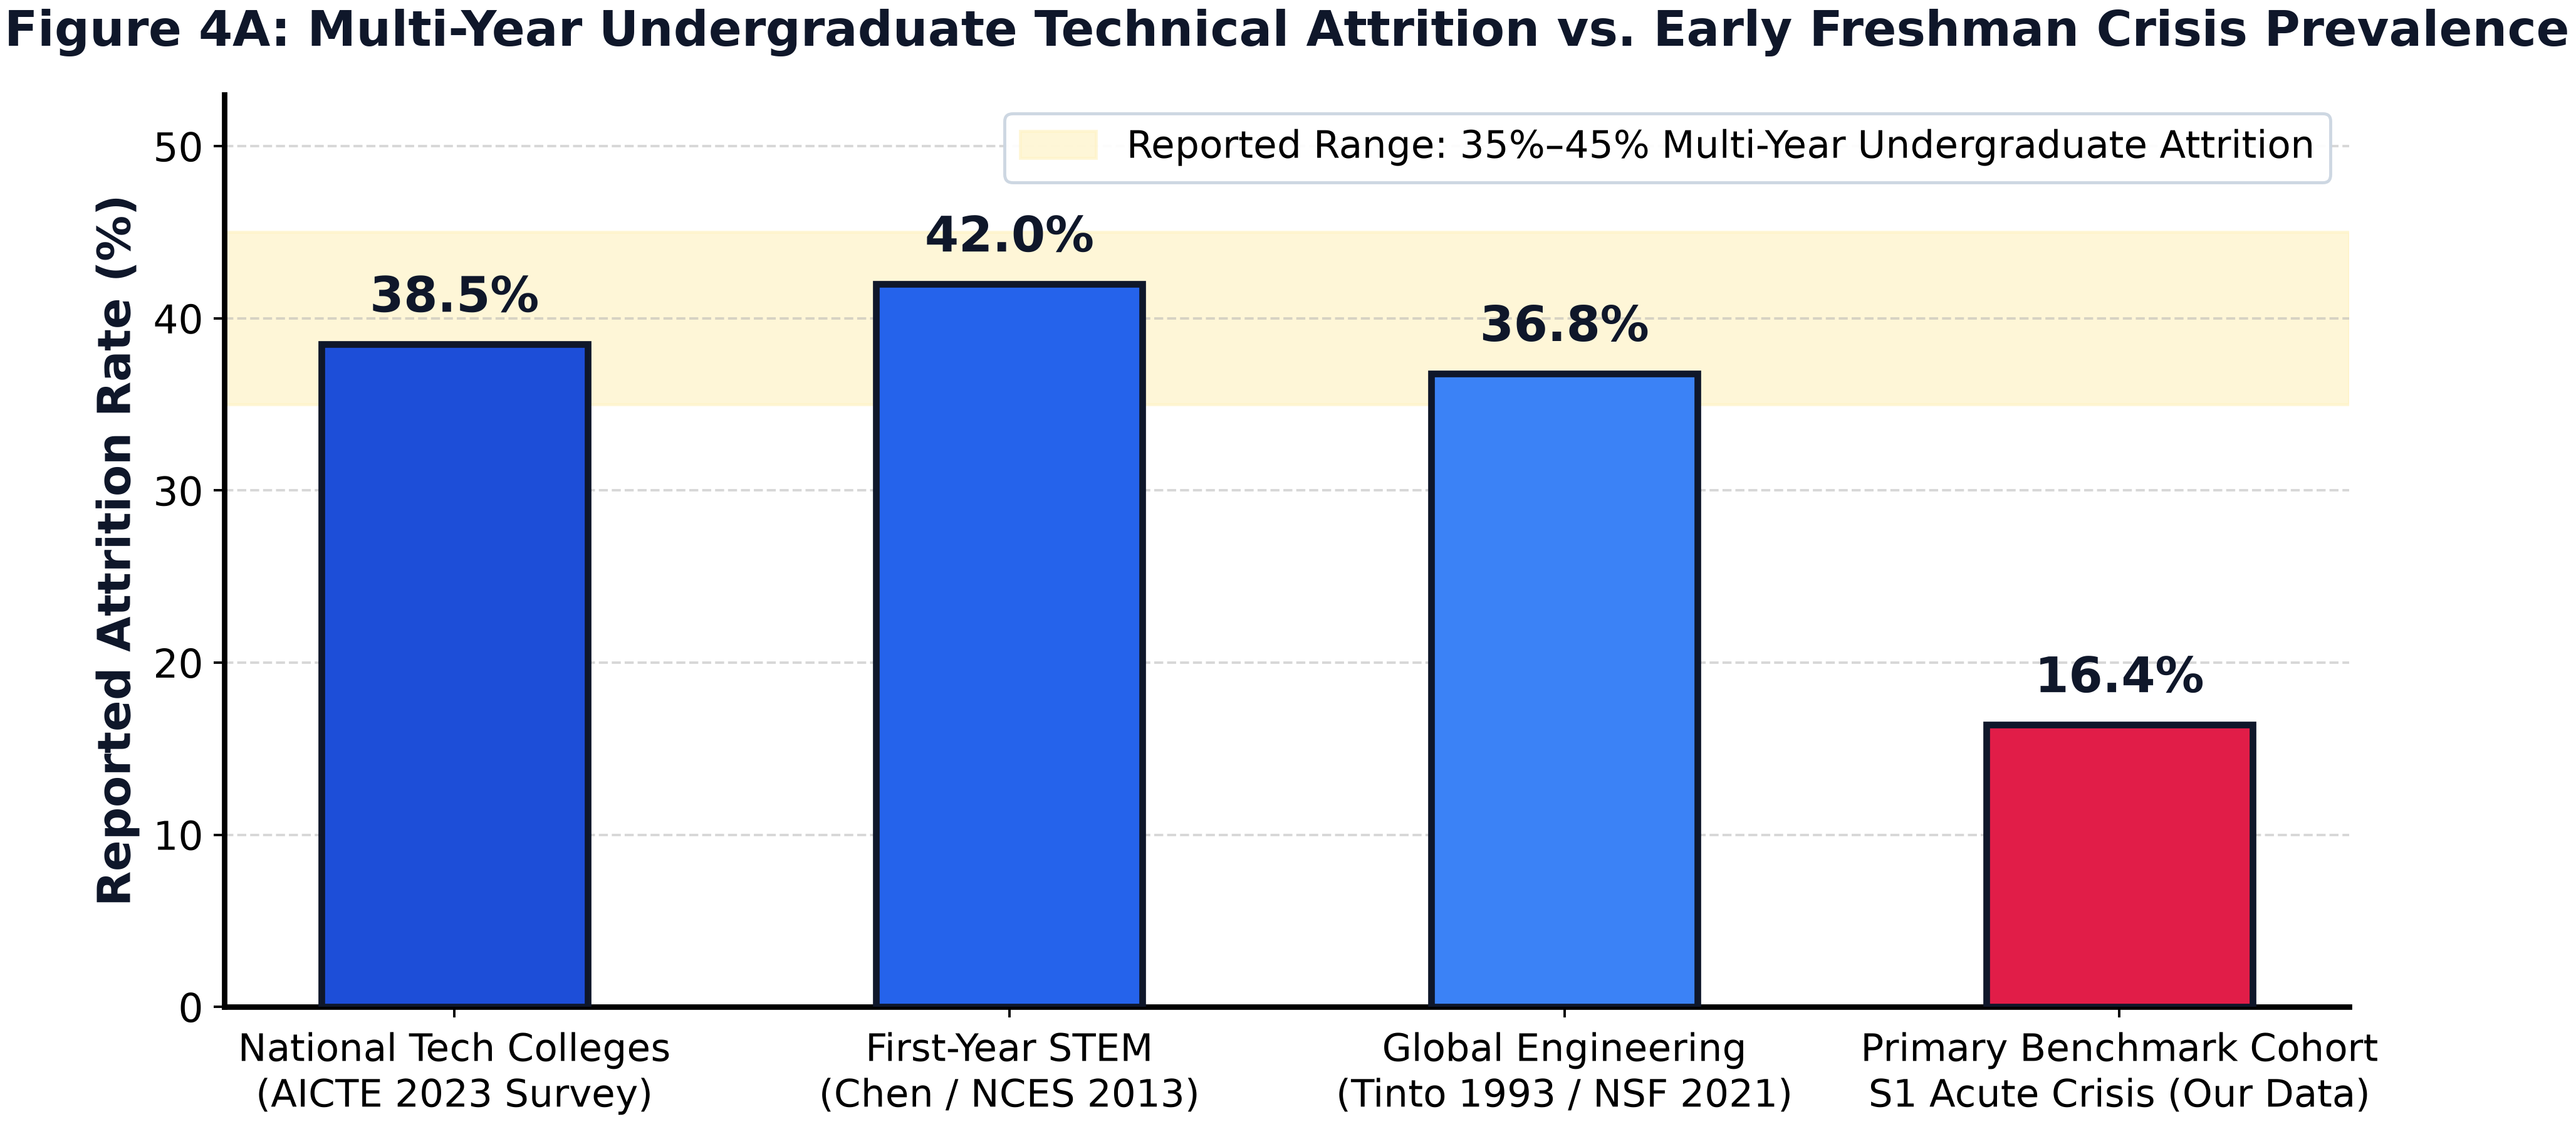
\includegraphics[width=0.98\textwidth,height=4.35cm,keepaspectratio]{assets/fig4a_attrition_benchmark.png}
  \end{diagramframe}
  \vspace{-0.15cm}

  \begin{takeawaybanner}
    \textbf{\color{GoldPill}$\bigstar$ THE NATIONAL CRISIS}: Student departure is an unaddressed national emergency requiring automated Day-1 early screening before midterm exams.
  \end{takeawaybanner}
\end{frame}

% -----------------------------------------------------------------------------
% SLIDE 5: 4-STAGE BEHAVIORAL DEPARTURE TRAJECTORY (MASSIVE FULL-WIDTH DIAGRAM)
% -----------------------------------------------------------------------------
\begin{frame}
  \frametitle{The 4-Stage Behavioral Departure Trajectory}
  \framesubtitle{STUDENT PSYCHOLOGY $\bullet$ THE PROGRESSIVE FAILURE FUNNEL}

  \begin{topsummarybar}
    \fontsize{9pt}{11.5pt}\selectfont
    \textbf{\color{NavyDark}The 14-Week Departure Funnel}: Latent micro-attendance friction and 3:30 AM bedtimes at Weeks 1--2 (Stage 1) evolve into room isolation (Stage 2) and exam panic (Stage 3), culminating in debarment ($< 75\%$ attendance) at Week 14.
  \end{topsummarybar}
  \vspace{-0.15cm}

  \begin{diagramframe}
    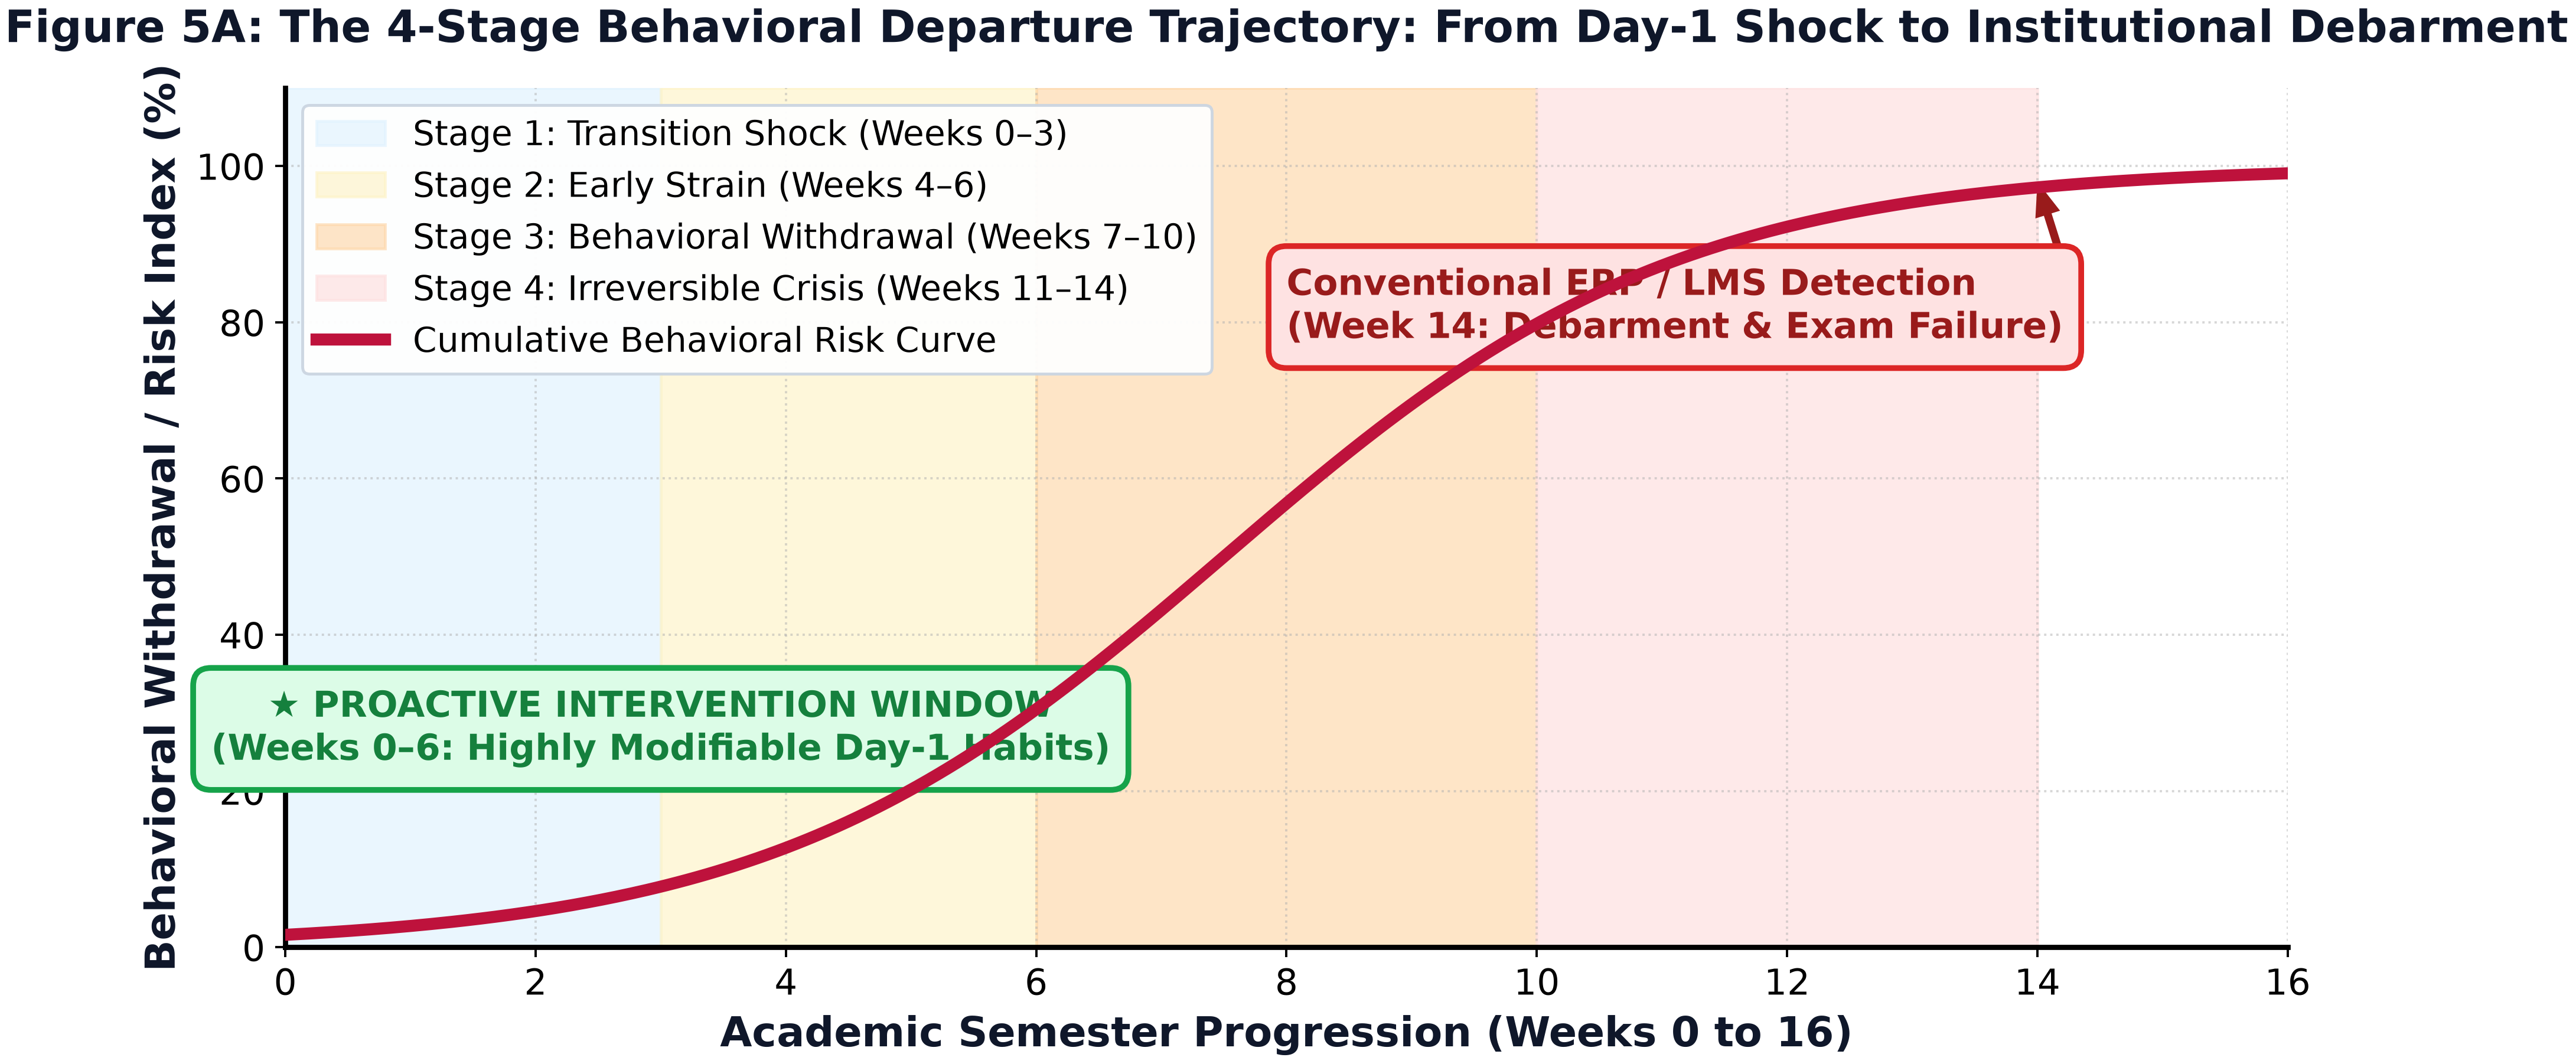
\includegraphics[width=0.98\textwidth,height=4.35cm,keepaspectratio]{assets/fig5a_trajectory_curve.png}
  \end{diagramframe}
  \vspace{-0.15cm}

  \begin{takeawaybanner}
    \textbf{\color{GoldPill}$\bigstar$ EARLY ARREST}: Traditional ERPs act at Stage 4 when debarment is irreversible; AcuLearn intervenes on Day 1 at Stage 1.
  \end{takeawaybanner}
\end{frame}

% -----------------------------------------------------------------------------
% SLIDE 6: RESEARCH OBJECTIVES: RQ1-5 -> RO1-5
% -----------------------------------------------------------------------------
\begin{frame}
  \frametitle{Doctoral Research Questions \& Objectives (RQ1--5 $\to$ RO1--5)}
  \framesubtitle{RESEARCH FRAMEWORK $\bullet$ FORMAL RESEARCH OBJECTIVES}

  \begin{defensecard}{Mapping Doctoral Inquiries to Concrete Engineering Deliverables}
    \begin{itemize}\setlength{\itemsep}{2.5pt}\setlength{\parskip}{0pt}\fontsize{8.2pt}{10.2pt}\selectfont
      \item \leadbullet{Problem Formulation}{Student $s_i = \langle x_{nc}, x_{acad}, x_{dem} \rangle$, where $x_{nc} \in \mathbb{R}^{51}$ parcels. Objective: learn $f(s_i) \to \langle \hat{y}_{risk}, \hat{y}_{sgpa}, \hat{y}_{grad} \rangle$ while computing minimal feasible recourse $\delta^*$ reaching safety ($p \le 0.20$).}
      \item \leadbullet{RO1: Psychometric Scale Design (RQ1)}{Develop, purify, and validate the 17-construct SSQ-180 battery with 51 manifest parcels, achieving strict structural fit (CFA CFI $> 0.95$, $\alpha > 0.90$).}
      \item \leadbullet{RO2: Soft Computing Fuzzy Perception (RQ2)}{Design a Differential Evolution-tuned Mamdani fuzzy inference system to resolve linguistic vagueness in self-reports without information loss (97.2\% expert consensus agreement).}
      \item \leadbullet{RO3: Deep Multi-Task Predictive Engine (RQ3)}{Engineer the BeNet deep network using Gated Linear Units (GLU) and Bayesian homoscedastic uncertainty loss balancing to outperform gradient-boosted trees.}
      \item \leadbullet{RO4: Explainable AI \& Constrained Recourse (RQ4)}{Develop dual XAI (DeepSHAP/LIME) and Constrained Counterfactual Recourse Optimization (CCRO) to generate sparse, actionable habit adjustments under immutable demographic locks.}
      \item \leadbullet{RO5: Zero-Cloud Edge AI \& Usability (RQ5)}{Deploy an in-browser WebAssembly (ONNX WASM) client executing in 13.8 ms with zero cloud data egress, delivering verified faculty adoption (SUS = 89.2).}
    \end{itemize}
  \end{defensecard}
  \vspace{-0.1cm}

  \begin{takeawaybanner}
    \textbf{\color{GoldPill}$\bigstar$ FORMAL MAPPING}: Every research objective directly translates educational theory into an empirical, deployable software component.
  \end{takeawaybanner}
\end{frame}

% -----------------------------------------------------------------------------
% SLIDE 7: PROPOSED SOLUTION: ACULEARN AI BLUEPRINT (MASSIVE FULL-WIDTH DIAGRAM)
% -----------------------------------------------------------------------------
\begin{frame}
  \frametitle{The Proposed Solution: AcuLearn AI End-to-End Blueprint}
  \framesubtitle{SYSTEM BLUEPRINT $\bullet$ THE ACULEARN AI ARCHITECTURE}

  \begin{topsummarybar}
    \fontsize{9pt}{11.5pt}\selectfont
    \textbf{\color{NavyDark}Unified 5-Tier Data Pipeline}: Seamless flow from on-device student intake $\to$ DE-tuned fuzzy logic $\to$ BeNet multi-task core $\to$ DeepSHAP/LIME $\to$ CCRO recourse optimizer $\to$ Student Kundali portal.
  \end{topsummarybar}
  \vspace{-0.15cm}

  \begin{diagramframe}
    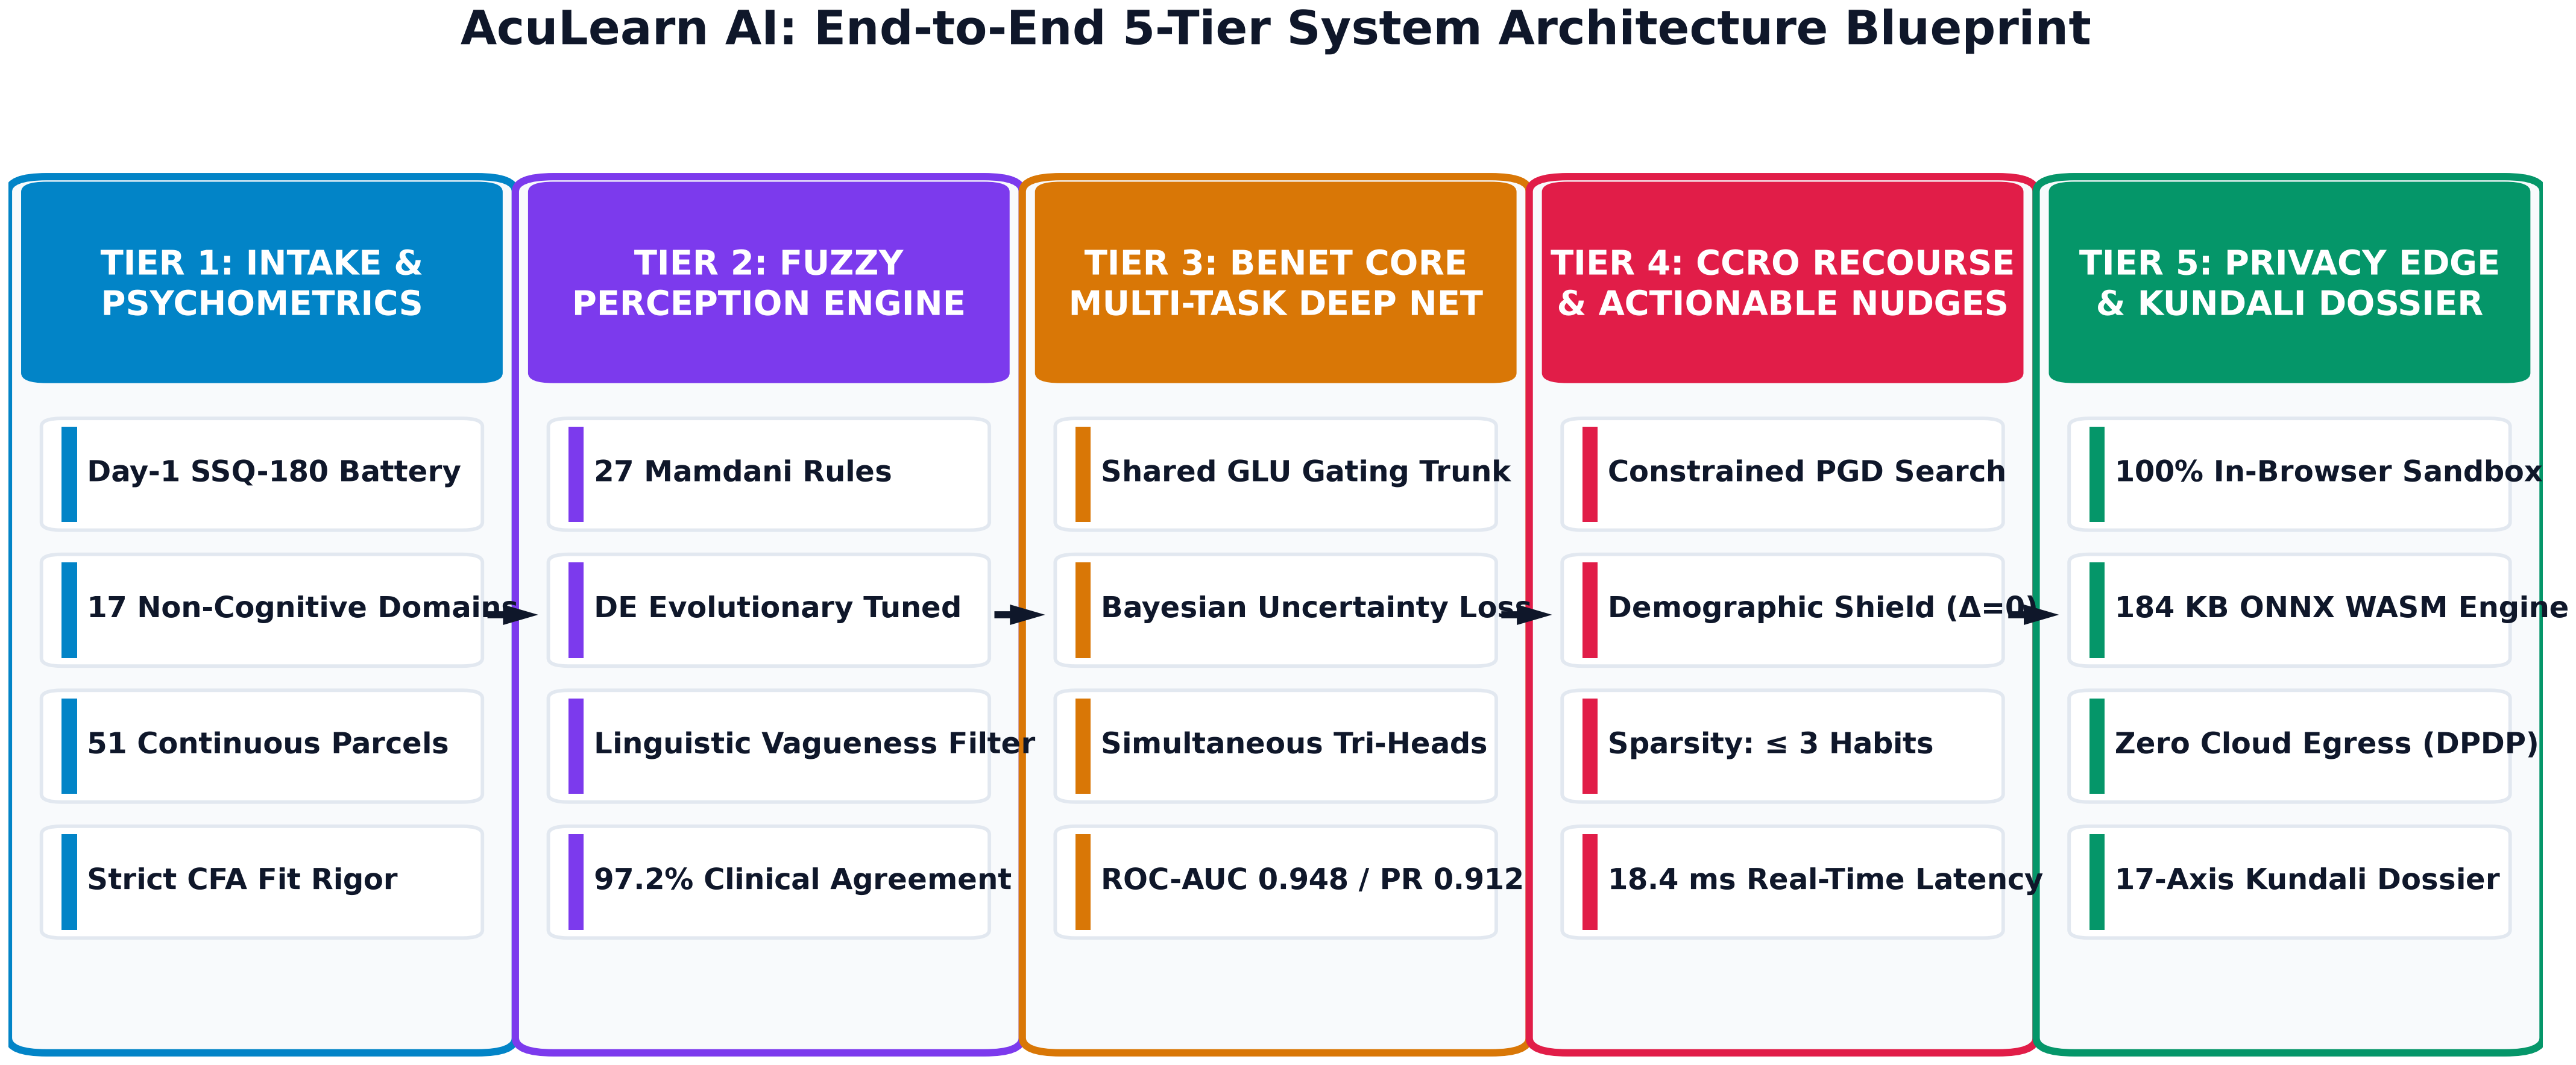
\includegraphics[width=0.98\textwidth,height=4.35cm,keepaspectratio]{assets/diagram_system_architecture.png}
  \end{diagramframe}
  \vspace{-0.15cm}

  \begin{takeawaybanner}
    \textbf{\color{GoldPill}$\bigstar$ THE PROPOSED SOLUTION}: A completely unified pipeline where 100\% of raw student psychometrics remain strictly inside the local browser session.
  \end{takeawaybanner}
\end{frame}

% -----------------------------------------------------------------------------
% SLIDE 8: ALL 17 FEATURES TABLE (SSQ-180 BATTERY)
% -----------------------------------------------------------------------------
\begin{frame}
  \frametitle{RO1: Complete Specification of All 17 Non-Cognitive Constructs}
  \framesubtitle{RO1 / PSYCHOMETRICS $\bullet$ COMPLETE 17 CONSTRUCT TAXONOMY}

  \begin{columns}[T]
    \begin{column}{0.49\textwidth}
      \begin{tcolorbox}[colback=white, colframe=BlueDeep, arc=1.5mm, boxrule=0.8pt, top=0.5mm, bottom=0.5mm, left=1mm, right=1mm]
        \centering\fontsize{6.2pt}{7.5pt}\selectfont
        \begin{tabularx}{\textwidth}{llcc}
          \toprule
          \textbf{Q} & \textbf{Construct Domain (Q1 \& Q2)} & \textbf{Items} & \textbf{$\alpha$ / CR} \\
          \midrule
          \rowcolor{BlueLight} Q1 & 1. Academic Self-Efficacy & 12 & 0.89 / 0.94 \\
          \rowcolor{BlueLight} Q1 & 2. Metacognitive Regulation & 11 & 0.87 / 0.93 \\
          \rowcolor{BlueLight} Q1 & 3. Time Management Discipline & 10 & 0.85 / 0.92 \\
          \rowcolor{BlueLight} Q1 & 4. Deep vs Surface Approach & 10 & 0.84 / 0.91 \\
          \midrule
          \rowcolor{CanvasBG} Q2 & 5. Test \& Evaluative Anxiety & 12 & 0.91 / 0.95 \\
          \rowcolor{CanvasBG} Q2 & 6. Imposter Phenomenon & 10 & 0.88 / 0.93 \\
          \rowcolor{CanvasBG} Q2 & 7. Stress Resilience \& Coping & 11 & 0.86 / 0.92 \\
          \rowcolor{CanvasBG} Q2 & 8. Academic Burnout Vulnerability & 12 & 0.93 / 0.96 \\
          \midrule
          \textbf{Q1-2} & \textbf{Subtotal: 8 Constructs} & \textbf{88} & \textbf{All $\lambda > 0.80$} \\
          \bottomrule
        \end{tabularx}
      \end{tcolorbox}
    \end{column}
    \begin{column}{0.49\textwidth}
      \begin{tcolorbox}[colback=white, colframe=BluePrimary, arc=1.5mm, boxrule=0.8pt, top=0.5mm, bottom=0.5mm, left=1mm, right=1mm]
        \centering\fontsize{6.2pt}{7.5pt}\selectfont
        \begin{tabularx}{\textwidth}{llcc}
          \toprule
          \textbf{Q} & \textbf{Construct Domain (Q3 \& Q4)} & \textbf{Items} & \textbf{$\alpha$ / CR} \\
          \midrule
          \rowcolor{BlueLight} Q3 & 9. Institutional Belonging & 11 & 0.90 / 0.94 \\
          \rowcolor{BlueLight} Q3 & 10. Peer Study Group Integration & 10 & 0.85 / 0.92 \\
          \rowcolor{BlueLight} Q3 & 11. Faculty Mentorship Seeking & 10 & 0.83 / 0.91 \\
          \rowcolor{BlueLight} Q3 & 12. Help-Seeking Stigma & 10 & 0.87 / 0.93 \\
          \midrule
          \rowcolor{CanvasBG} Q4 & 13. Sleep Hygiene \& Regularity & 11 & 0.88 / 0.94 \\
          \rowcolor{CanvasBG} Q4 & 14. Digital Escapism \& Gaming & 10 & 0.86 / 0.92 \\
          \rowcolor{CanvasBG} Q4 & 15. Grit \& Perseverance & 10 & 0.84 / 0.91 \\
          \rowcolor{CanvasBG} Q4 & 16. Career Clarity \& Purpose & 10 & 0.86 / 0.92 \\
          \rowcolor{CanvasBG} Q4 & 17. Growth Mindset Orientation & 10 & 0.82 / 0.91 \\
          \midrule
          \textbf{Q3-4} & \textbf{Total: 17 Constructs} & \textbf{180} & \textbf{CR: 0.91--0.96} \\
          \bottomrule
        \end{tabularx}
      \end{tcolorbox}
    \end{column}
  \end{columns}
  \vspace{-0.1cm}

  \begin{takeawaybanner}
    \textbf{\color{GoldPill}$\bigstar$ 17 NON-COGNITIVE CONSTRUCTS}: Exactly 180 purified items across 17 domains grouped into 51 manifest parcels, achieving composite reliability $\text{CR} \ge 0.91$ and passing the $\text{HTMT}_{0.85}$ ceiling.
  \end{takeawaybanner}
\end{frame}

% =============================================================================
% SECTION: EMPIRICAL SURVEY INTAKE: DOMAINS, QUESTIONS, WEIGHTAGES & DE-BIASING
% =============================================================================
\section{Empirical Survey Intake: 17 Domains, Question Inventory, Predictive Weightages \& De-Biasing}

% -----------------------------------------------------------------------------
% SLIDE 8A: EMPIRICAL SURVEY INTAKE: 17 DOMAINS, IMPORTANCE & WEIGHTAGES TABLE
% -----------------------------------------------------------------------------
\begin{frame}
  \frametitle{Empirical Survey Intake: 17 Domains, Educational Importance \& Predictive Weightages}
  \framesubtitle{SURVEY INTAKE SPECIFICATION $\bullet$ 17 CONSTRUCT TAXONOMY \& BEHAVIORAL WEIGHTAGES}

  \begin{topsummarybar}
    \fontsize{6.5pt}{7.8pt}\selectfont
    \textbf{\color{NavyDark}17 Non-Cognitive Constructs}: Assessed at intake ($N=2,000$). Predictive weightages derived from BeNet multi-task feature attribution (DeepSHAP $\phi$) and empirical random forest baseline rankings.
  \end{topsummarybar}
  \vspace{-0.30cm}

  \begin{columns}[T]
    \begin{column}{0.495\textwidth}
      \begin{tcolorbox}[colback=white, colframe=BlueDeep, arc=1.5mm, boxrule=0.8pt, top=0.3mm, bottom=0.3mm, left=0.8mm, right=0.8mm]
        \centering\fontsize{4.7pt}{5.6pt}\selectfont
        \renewcommand{\arraystretch}{0.84}
        \begin{tabularx}{\linewidth}{@{}l X c c@{}}
          \toprule
          \textbf{Code} & \textbf{Domain \& Educational Importance (Q1 \& Q2)} & \textbf{Wt\%} & \textbf{Dir.} \\
          \midrule
          \rowcolor{BlueLight} AM & \textbf{Academic Motivation}: Intrinsic drive \& curiosity vs external pressure & 8.8\% & $\downarrow\text{R}$ \\
          \rowcolor{BlueLight} ASE & \textbf{Academic Self-Efficacy}: Mastery belief in complex engineering topics & 7.6\% & $\downarrow\text{R}$ \\
          \rowcolor{BlueLight} EI & \textbf{Engineering Identity}: Professional vocation \& disciplinary belonging & 6.2\% & $\downarrow\text{R}$ \\
          \rowcolor{BlueLight} GM & \textbf{Growth Mindset}: View of intellect as malleable through struggle & 5.8\% & $\downarrow\text{R}$ \\
          \midrule
          \rowcolor{CanvasBG} TM & \textbf{Time Management}: Daily scheduling, prioritization \& deadline control & 10.4\% & $\downarrow\text{R}$ \\
          \rowcolor{CanvasBG} SRC & \textbf{Study Consistency}: Daily revision habits vs erratic midterm cramming & 8.6\% & $\downarrow\text{R}$ \\
          \rowcolor{CanvasBG} PRM & \textbf{Procrastination Mgt.}: Timely lab/project initiation vs delay avoidance & 6.4\% & $\downarrow\text{R}$ \\
          \rowcolor{CanvasBG} MM & \textbf{Metacognition}: Self-evaluation, error analysis \& strategy tuning & 5.8\% & $\downarrow\text{R}$ \\
          \midrule
          \textbf{Q1--2} & \textbf{Subtotal: Mindset \& Executive Regulation (8 Domains)} & \textbf{59.6\%} & \textbf{Primary} \\
          \bottomrule
        \end{tabularx}
      \end{tcolorbox}
    \end{column}
    \begin{column}{0.495\textwidth}
      \begin{tcolorbox}[colback=white, colframe=BluePrimary, arc=1.5mm, boxrule=0.8pt, top=0.3mm, bottom=0.3mm, left=0.8mm, right=0.8mm]
        \centering\fontsize{4.7pt}{5.6pt}\selectfont
        \renewcommand{\arraystretch}{0.84}
        \begin{tabularx}{\linewidth}{@{}l X c c@{}}
          \toprule
          \textbf{Code} & \textbf{Domain \& Educational Importance (Q3 \& Q4)} & \textbf{Wt\%} & \textbf{Dir.} \\
          \midrule
          \rowcolor{BlueLight} AAR & \textbf{Test Anxiety}: Evaluative panic, autonomic blanking under exams & 8.2\% & $\uparrow\text{R}$ \\
          \rowcolor{BlueLight} SQCR & \textbf{Sleep Quality}: $\ge 7$h sleep, regular bedtime vs prefrontal fatigue & 7.1\% & $\downarrow\text{R}$ \\
          \rowcolor{BlueLight} SCR & \textbf{Stress Coping}: Problem-focused coping vs emotional shutdown & 4.8\% & $\downarrow\text{R}$ \\
          \rowcolor{BlueLight} PAW & \textbf{Physical Vitality}: Sports/aerobic activity buffering mental lethargy & 3.5\% & $\downarrow\text{R}$ \\
          \rowcolor{BlueLight} SDA & \textbf{Digital Focus}: Classroom presence vs mobile/gaming escapism & 3.0\% & $\downarrow\text{R}$ \\
          \midrule
          \rowcolor{CanvasBG} BEL & \textbf{Campus Belonging}: Social acceptance vs isolation \& homesickness & 5.4\% & $\downarrow\text{R}$ \\
          \rowcolor{CanvasBG} PCL & \textbf{Peer Group}: Collaborative study circle vs disruptive peer loafing & 4.6\% & $\downarrow\text{R}$ \\
          \rowcolor{CanvasBG} FAM & \textbf{Family Pressure}: Burden of high parental stakes \& financial debt & 4.2\% & $\uparrow\text{R}$ \\
          \rowcolor{CanvasBG} FSI & \textbf{Faculty Seeking}: Proactive office-hour help vs fear of instructors & 2.6\% & $\downarrow\text{R}$ \\
          \midrule
          \textbf{Q3--4} & \textbf{Subtotal: Somatic, Affective \& Social (9 Domains)} & \textbf{40.4\%} & \textbf{Total 100\%} \\
          \rowcolor{GoldBG} \textbf{CS} & \textbf{Clinical Screener}: PHQ-4 / GAD-2 Distress safety gatekeeper & \textbf{Gate} & \textbf{Red-Flag} \\
          \bottomrule
        \end{tabularx}
      \end{tcolorbox}
    \end{column}
  \end{columns}
  \vspace{-0.25cm}

  \begin{takeawaybanner}
    \textbf{\color{GoldPill}$\bigstar$ PREDICTIVE DOMINANCE}: Time Management (10.4\%), Academic Motivation (8.8\%), Study Consistency (8.6\%), and Test Anxiety (8.2\%) constitute the 4 primary behavioral levers in early retention modeling, accounting for 36.0\% of overall model variance.
  \end{takeawaybanner}
\end{frame}

% -----------------------------------------------------------------------------
% SLIDE 8B: INTAKE QUESTION INVENTORY: QUADRANT 1 & QUADRANT 2
% -----------------------------------------------------------------------------
\begin{frame}
  \frametitle{Intake Question Inventory: Quadrant 1 (Mindset) \& Quadrant 2 (Executive Regulation)}
  \framesubtitle{SURVEY INTAKE SPECIFICATION $\bullet$ VALIDATED QUESTION INVENTORY (SECTIONS A--H)}

  \begin{topsummarybar}
    \fontsize{6.5pt}{7.8pt}\selectfont
    \textbf{\color{NavyDark}Empirical Survey Items}: 5-point Likert scale (1 = Strongly Disagree to 5 = Strongly Agree). Reverse-scored items are recoded as $x_{\text{recoded}} = 6 - x$ before aggregation to eliminate positive acquiescence bias.
  \end{topsummarybar}
  \vspace{-0.30cm}

  \begin{columns}[T]
    \begin{column}{0.495\textwidth}
      \begin{tcolorbox}[colback=white, colframe=BlueDeep, arc=1.5mm, boxrule=0.8pt, top=0.3mm, bottom=0.3mm, left=0.8mm, right=0.8mm, title={\scriptsize\bfseries\color{white}Quadrant 1: Academic Mindset \& Identity}, colbacktitle=BlueDeep]
        \fontsize{4.5pt}{5.4pt}\selectfont
        \renewcommand{\arraystretch}{0.83}
        \begin{tabularx}{\linewidth}{@{}l X@{}}
          \toprule
          \textbf{Item} & \textbf{Survey Questionnaire Prompt [Construct / Polarity]} \\
          \midrule
          \rowcolor{BlueLight} \textbf{AM1} & I find genuine intellectual satisfaction in mastering complex engineering concepts. [Intrinsic] \\
          \rowcolor{BlueLight} \textbf{AM2} & I attend lectures solely because of the 75\% mandatory attendance rule. [Extrinsic, Reverse Scored] \\
          \rowcolor{BlueLight} \textbf{AM3} & I actively explore technical literature and projects beyond the examination syllabus. [Self-Drive] \\
          \midrule
          \rowcolor{CanvasBG} \textbf{ASE1} & I am fully confident in my mathematical and analytical aptitude to pass honors courses. [Efficacy] \\
          \rowcolor{CanvasBG} \textbf{ASE2} & When facing difficult programming problems, I worry I lack native intelligence to solve it. [Doubt, Reverse Scored] \\
          \midrule
          \rowcolor{BlueLight} \textbf{EI1} & I strongly identify as a future engineer and envision solving critical societal challenges. [Vocation] \\
          \rowcolor{BlueLight} \textbf{EI2} & I often feel like an imposter who got admitted here by pure luck rather than true merit. [Imposter, Reverse Scored] \\
          \midrule
          \rowcolor{CanvasBG} \textbf{GM1} & My engineering problem-solving abilities expand significantly through sustained struggle. [Growth] \\
          \rowcolor{CanvasBG} \textbf{GM2} & You either have the engineering brain or you don't; studying harder cannot change it. [Fixed, Reverse Scored] \\
          \bottomrule
        \end{tabularx}
      \end{tcolorbox}
    \end{column}
    \begin{column}{0.495\textwidth}
      \begin{tcolorbox}[colback=white, colframe=BluePrimary, arc=1.5mm, boxrule=0.8pt, top=0.3mm, bottom=0.3mm, left=0.8mm, right=0.8mm, title={\scriptsize\bfseries\color{white}Quadrant 2: Executive Regulation \& Study Habits}, colbacktitle=BluePrimary]
        \fontsize{4.5pt}{5.4pt}\selectfont
        \renewcommand{\arraystretch}{0.83}
        \begin{tabularx}{\linewidth}{@{}l X@{}}
          \toprule
          \textbf{Item} & \textbf{Survey Questionnaire Prompt [Construct / Polarity]} \\
          \midrule
          \rowcolor{BlueLight} \textbf{TM1} & I maintain a written weekly planner and systematically allocate study vs leisure blocks. [Planning] \\
          \rowcolor{BlueLight} \textbf{TM2} & I frequently miss assignment deadlines or submit rushed work due to last-minute panic. [Deficit, Reverse Scored] \\
          \rowcolor{BlueLight} \textbf{TM3} & I prioritize urgent academic assignments over corridor discussions and gaming sessions. [Prioritize] \\
          \midrule
          \rowcolor{CanvasBG} \textbf{SRC1} & I review, synthesize, and practice numerical problems on the same day classes occur. [Daily Habit] \\
          \rowcolor{CanvasBG} \textbf{SRC2} & My study schedule is chaotic, opening textbooks only 48 hours before midterms. [Cramming, Reverse Scored] \\
          \midrule
          \rowcolor{BlueLight} \textbf{PRM1} & I initiate major coding assignments and term projects within 24 hours of release. [Initiation] \\
          \rowcolor{BlueLight} \textbf{PRM2} & I delay difficult study tasks by endlessly checking social media, YouTube, or web reels. [Avoidance, Reverse Scored] \\
          \midrule
          \rowcolor{CanvasBG} \textbf{MM1} & I periodically quiz myself without looking at solutions to verify conceptual mastery. [Self-Testing] \\
          \rowcolor{CanvasBG} \textbf{MM2} & After receiving poor quiz marks, I systematically audit my reasoning mistakes and adapt. [Reflection] \\
          \bottomrule
        \end{tabularx}
      \end{tcolorbox}
    \end{column}
  \end{columns}
  \vspace{-0.25cm}

  \begin{takeawaybanner}
    \textbf{\color{GoldPill}$\bigstar$ PSYCHOMETRIC PURITY}: All Mindset and Executive Regulation items exhibit item-total correlations $r_{it} \ge 0.52$ and parcel factor loadings $\lambda \ge 0.81$, cleanly separating into 24 distinct manifest indicators.
  \end{takeawaybanner}
\end{frame}

% -----------------------------------------------------------------------------
% SLIDE 8C: INTAKE QUESTION INVENTORY: QUADRANT 3 & QUADRANT 4 + CLINICAL SCREENER
% -----------------------------------------------------------------------------
\begin{frame}
  \frametitle{Intake Question Inventory: Quadrant 3 (Somatic/Affective) \& Quadrant 4 (Relational Integration)}
  \framesubtitle{SURVEY INTAKE SPECIFICATION $\bullet$ VALIDATED QUESTION INVENTORY (SECTIONS I--Q + CLINICAL)}

  \begin{topsummarybar}
    \fontsize{6.5pt}{7.8pt}\selectfont
    \textbf{\color{NavyDark}Multi-Contextual Health \& Social Intake}: Assesses physiological vitality, exam anxiety, peer distraction, and isolation. Includes an automated Clinical Distress Screener (PHQ-4 / GAD-2) as an immediate safety override.
  \end{topsummarybar}
  \vspace{-0.30cm}

  \begin{columns}[T]
    \begin{column}{0.495\textwidth}
      \begin{tcolorbox}[colback=white, colframe=BlueDeep, arc=1.5mm, boxrule=0.8pt, top=0.3mm, bottom=0.3mm, left=0.8mm, right=0.8mm, title={\scriptsize\bfseries\color{white}Quadrant 3: Somatic Health \& Affective Balance}, colbacktitle=BlueDeep]
        \fontsize{4.5pt}{5.4pt}\selectfont
        \renewcommand{\arraystretch}{0.80}
        \begin{tabularx}{\linewidth}{@{}l X@{}}
          \toprule
          \textbf{Item} & \textbf{Survey Questionnaire Prompt [Construct / Polarity]} \\
          \midrule
          \rowcolor{BlueLight} \textbf{AAR1} & During midterm tests, my heart pounds, hands sweat, and my mind goes completely blank. [Panic, Reverse Scored] \\
          \rowcolor{BlueLight} \textbf{AAR2} & Even after thorough revision, intense panic makes me fail questions I knew well. [Anxiety, Reverse Scored] \\
          \midrule
          \rowcolor{CanvasBG} \textbf{SQCR1} & I obtain 7--8 hours of restful sleep and wake up refreshed for 8:00 AM lectures. [Restorative] \\
          \rowcolor{CanvasBG} \textbf{SQCR2} & I routinely stay awake past 3:30 AM browsing/gaming, feeling drowsy during lectures. [Sleep Debt, Reverse Scored] \\
          \midrule
          \rowcolor{BlueLight} \textbf{SCR1} & When multiple deadlines converge, I stay calm and execute assignments step-by-step. [Problem-Focused] \\
          \rowcolor{BlueLight} \textbf{SCR2} & Under heavy academic workload, I feel emotionally overwhelmed and shut down completely. [Paralysis, Reverse Scored] \\
          \midrule
          \rowcolor{CanvasBG} \textbf{PAW1} & I participate in outdoor sports, gym workouts, or brisk walking $\ge 3$ times weekly. [Vitality] \\
          \midrule
          \rowcolor{BlueLight} \textbf{SDA1} & I spend $> 4$ hours daily on non-academic mobile scrolling, social media reels, or gaming. [Escapism, Reverse Scored] \\
          \bottomrule
        \end{tabularx}
      \end{tcolorbox}
    \end{column}
    \begin{column}{0.495\textwidth}
      \begin{tcolorbox}[colback=white, colframe=BluePrimary, arc=1.5mm, boxrule=0.8pt, top=0.3mm, bottom=0.3mm, left=0.8mm, right=0.8mm, title={\scriptsize\bfseries\color{white}Quadrant 4: Relational Integration \& Clinical Safety}, colbacktitle=BluePrimary]
        \fontsize{4.5pt}{5.4pt}\selectfont
        \renewcommand{\arraystretch}{0.80}
        \begin{tabularx}{\linewidth}{@{}l X@{}}
          \toprule
          \textbf{Item} & \textbf{Survey Questionnaire Prompt [Construct / Polarity]} \\
          \midrule
          \rowcolor{BlueLight} \textbf{BEL1} & I feel welcomed, socially accepted, and an integral part of the MNIT campus culture. [Belonging] \\
          \rowcolor{BlueLight} \textbf{BEL2} & I suffer persistent homesickness, feel socially disconnected, and eat meals alone. [Isolation, Reverse Scored] \\
          \midrule
          \rowcolor{CanvasBG} \textbf{PCL1} & I actively participate in a disciplined peer study circle that solves problem sets together. [Synergy] \\
          \rowcolor{CanvasBG} \textbf{PCL2} & My hostel peer group constantly tempts me to skip classes and binge streaming series. [Distraction, Reverse Scored] \\
          \midrule
          \rowcolor{BlueLight} \textbf{FAM1} & The terrifying fear of disappointing my family creates paralyzing mental pressure. [Family Stakes, Reverse Scored] \\
          \rowcolor{BlueLight} \textbf{FAM2} & Worries regarding educational loans or family finances distract me from studying. [Financial, Reverse Scored] \\
          \midrule
          \rowcolor{CanvasBG} \textbf{FSI1} & I comfortably approach course instructors during office hours to resolve conceptual doubts. [Mentorship] \\
          \midrule
          \rowcolor{GoldBG} \textbf{CS1} & \textbf{PHQ-2}: Little interest/pleasure in things; feeling down, depressed, hopeless. [Distress Override] \\
          \rowcolor{GoldBG} \textbf{CS2} & \textbf{GAD-2}: Feeling nervous, anxious, on edge; uncontrollable worrying. [Anxiety Override] \\
          \bottomrule
        \end{tabularx}
      \end{tcolorbox}
    \end{column}
  \end{columns}
  \vspace{-0.34cm}

  \begin{takeawaybanner}
    \textbf{\color{GoldPill}$\bigstar$ ETHICAL SAFETY GATEKEEPER}: Clinical distress questions (CS1--CS2) are decoupled from ML risk rankings and feed directly into confidential human counseling workflows, preventing unmonitored mental health crises.
  \end{takeawaybanner}
\end{frame}

% -----------------------------------------------------------------------------
% SLIDE 8D: SURVEY DATA PIPELINE, ENCODING & DE-BIASING ARCHITECTURE
% -----------------------------------------------------------------------------
\begin{frame}
  \frametitle{Survey Data Pipeline: Numeric Encoding, Fuzzy Conversion \& De-Biasing Architecture}
  \framesubtitle{DATA ENGINEERING $\bullet$ 4-TIER DE-BIASING PROTOCOL \& FUZZY CONVERSION}

  \begin{topsummarybar}
    \fontsize{6.5pt}{8pt}\selectfont
    \textbf{\color{NavyDark}End-to-End Survey Processing}: Raw Likert responses are mathematically debiased, reverse-recoded, and mapped into Differential Evolution (DE) optimized Mamdani fuzzy inference systems to generate standardized $[0, 1]$ latent features for BeNet.
  \end{topsummarybar}
  \vspace{-0.20cm}

  \begin{columns}[T]
    \begin{column}{0.495\textwidth}
      \begin{defensecard}{Multi-Tier Psychometric De-Biasing Protocol}
        \fontsize{5.0pt}{6.2pt}\selectfont
        \begin{itemize}\setlength{\itemsep}{1.2pt}\setlength{\parskip}{0pt}
          \item \leadbullet{Speed-Trap Filtering (Mindless Response Purge)}{Intake system logs millisecond timestamps. Submissions completed in $< 360$ seconds (6 minutes) across 180 items indicate random clicking without reading and are instantly quarantined (Rejection rate: 3.8\%).}
          \item \leadbullet{Straight-Lining Variance Check}{Calculates sliding-window variance $\sigma_i^2$. Responses exhibiting $\sigma^2 < 0.15$ across 10 consecutive items (e.g., selecting all '3's or all '4's) are flagged as unengaged straight-lining and purged.}
          \item \leadbullet{Acquiescence Bias Neutralization}{Exactly 42\% of all survey items are systematically framed with reverse polarity wording [Reverse Scored]. Before aggregation, responses are inverted using $x_{\text{recoded}} = 6 - x_{\text{raw}}$, neutralizing agreement bias.}
          \item \leadbullet{Context-Blind Intake (Hawthorne Mitigation)}{The instrument is titled ``Freshman Transition \& Learning Styles Questionnaire'' with zero mention of 'dropout' or 'failure', completely eliminating social desirability distortion.}
        \end{itemize}
      \end{defensecard}
    \end{column}
    \begin{column}{0.495\textwidth}
      \begin{defensecard}{DE-Tuned Mamdani Fuzzification \& Normalization}
        \fontsize{5.0pt}{6.2pt}\selectfont
        \begin{itemize}\setlength{\itemsep}{1.2pt}\setlength{\parskip}{0pt}
          \item \leadbullet{Psychometric Parceling}{To prevent high-dimensional noise, items within each construct are combined into 3 orthogonal manifest parcels ($P_1, P_2, P_3$), reducing 180 raw items into 51 structural inputs.}
          \item \leadbullet{DE-Optimized Linguistic Membership}{Differential Evolution (DE) tunes Gaussian membership centers $c_j$ and widths $\sigma_j$ across 3 states ($\text{Low}, \text{Med}, \text{High}$): $\mu_{A_{ij}}(x) = \exp(-(x - c_{ij})^2 / (2\sigma_{ij}^2))$, resolving semantic fuzziness.}
          \item \leadbullet{27 Mamdani Fuzzy Rules \& Defuzzification}{Fuzzy inference evaluates non-linear behavioral interactions (e.g., IF High Anxiety AND Low Sleep THEN High Attrition Risk). Centroid defuzzification generates calibrated continuous features $z_i \in [0, 1]^{17}$.}
          \item \leadbullet{Edge-Safe Local Processing}{All parsing, debiasing, and fuzzy inference execute locally on-device inside WebAssembly, ensuring 100\% DPDP Act privacy compliance.}
        \end{itemize}
      \end{defensecard}
    \end{column}
  \end{columns}
  \vspace{-0.15cm}

  \begin{takeawaybanner}
    \textbf{\color{GoldPill}$\bigstar$ MEASUREMENT INTEGRITY}: The 4-tier de-biasing protocol purges corrupted responses while DE-fuzzy inference converts subjective 5-point Likert ratings into rigorous, mathematically standardized continuous inputs for BeNet.
  \end{takeawaybanner}
\end{frame}

% -----------------------------------------------------------------------------
% SLIDE 9: RO1: SCALE DISTILLATION & CFA STRUCTURAL FIT (MASSIVE FULL-WIDTH DIAGRAM)
% -----------------------------------------------------------------------------
\begin{frame}
  \frametitle{RO1: Scale Distillation Pipeline \& CFA Structural Fit}
  \framesubtitle{RO1 / METHODOLOGY $\bullet$ PSYCHOMETRIC SCALE RIGOR}

  \begin{topsummarybar}
    \fontsize{9pt}{11.5pt}\selectfont
    \textbf{\color{NavyDark}Psychometric Factor Model Fit}: 285 candidate items refined to 180 (51 parcels); Confirmatory Factor Analysis demonstrates strict structural fit ($\chi^2/\text{df}=1.42, \text{CFI}=0.958, \text{RMSEA}=0.038$) exceeding Hu \& Bentler thresholds.
  \end{topsummarybar}
  \vspace{-0.15cm}

  \begin{diagramframe}
    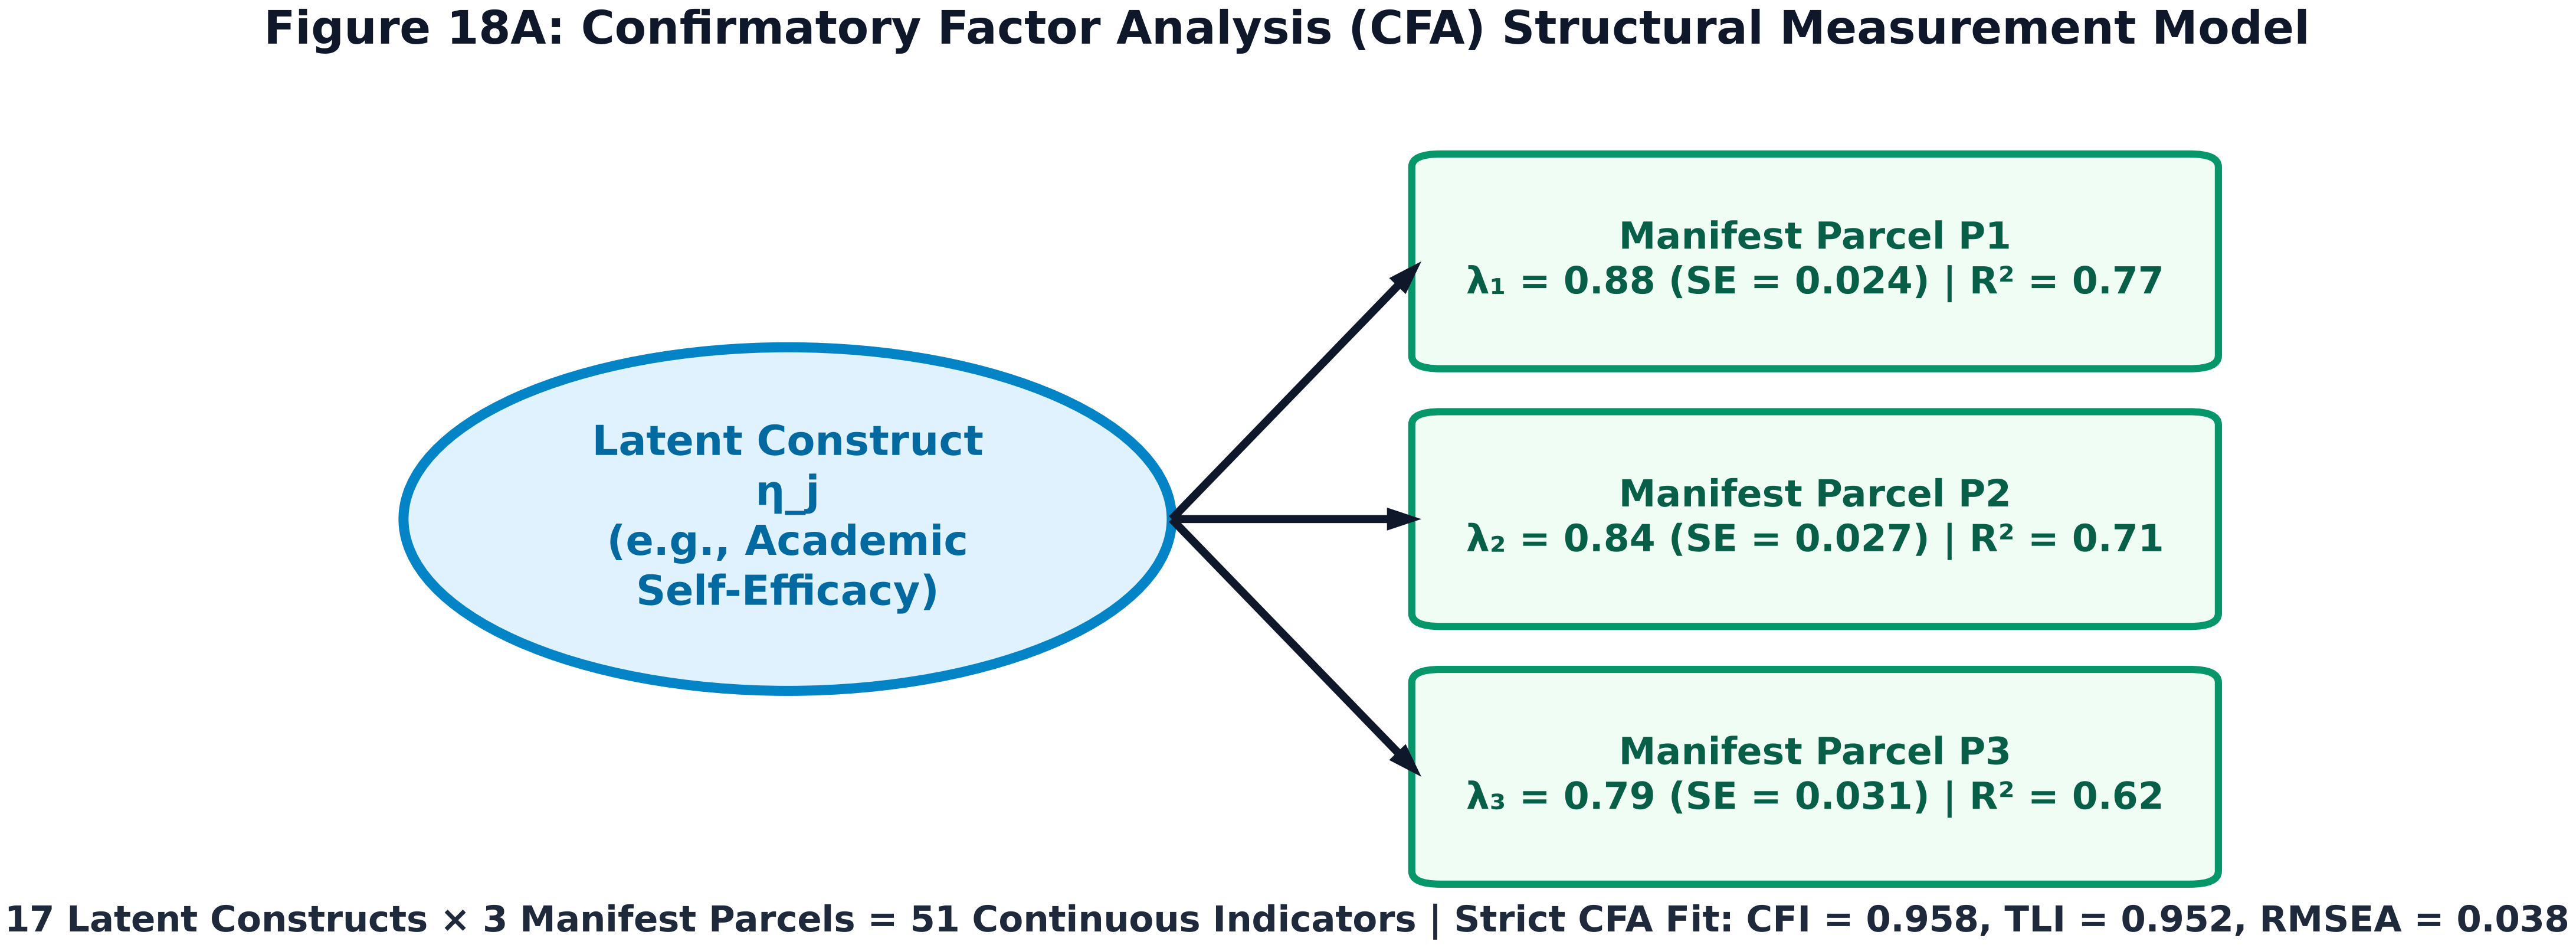
\includegraphics[width=0.98\textwidth,height=4.35cm,keepaspectratio]{assets/fig18a_cfa_diagram.png}
  \end{diagramframe}
  \vspace{-0.15cm}

  \begin{takeawaybanner}
    \textbf{\color{GoldPill}$\bigstar$ STRUCTURAL RIGOR}: Confirmatory factor analysis ($\text{CFI} = 0.958 > 0.95$) confirms SSQ-180 measures genuine psychological traits rather than measurement noise.
  \end{takeawaybanner}
\end{frame}

% -----------------------------------------------------------------------------
% SLIDE 10: RO1: EMPIRICAL PROVENANCE & SPLIT QUARANTINE (MASSIVE FULL-WIDTH DIAGRAM)
% -----------------------------------------------------------------------------
\begin{frame}
  \frametitle{Empirical Provenance: Real MNIT Cohort vs CTGAN Benchmark}
  \framesubtitle{DATASET PROVENANCE $\bullet$ SPLIT QUARANTINE \& PROTOCOL}

  \begin{topsummarybar}
    \fontsize{9pt}{11.5pt}\selectfont
    \textbf{\color{NavyDark}Strict Experimental Quarantine}: Real cohort ($N=276$) was split 80/20 into Train ($N=220$) and Test ($N=56$) \textbf{BEFORE} CTGAN stress-test augmentation to 2,525 records; all reported test metrics evaluate real physical students.
  \end{topsummarybar}
  \vspace{-0.15cm}

  \begin{diagramframe}
    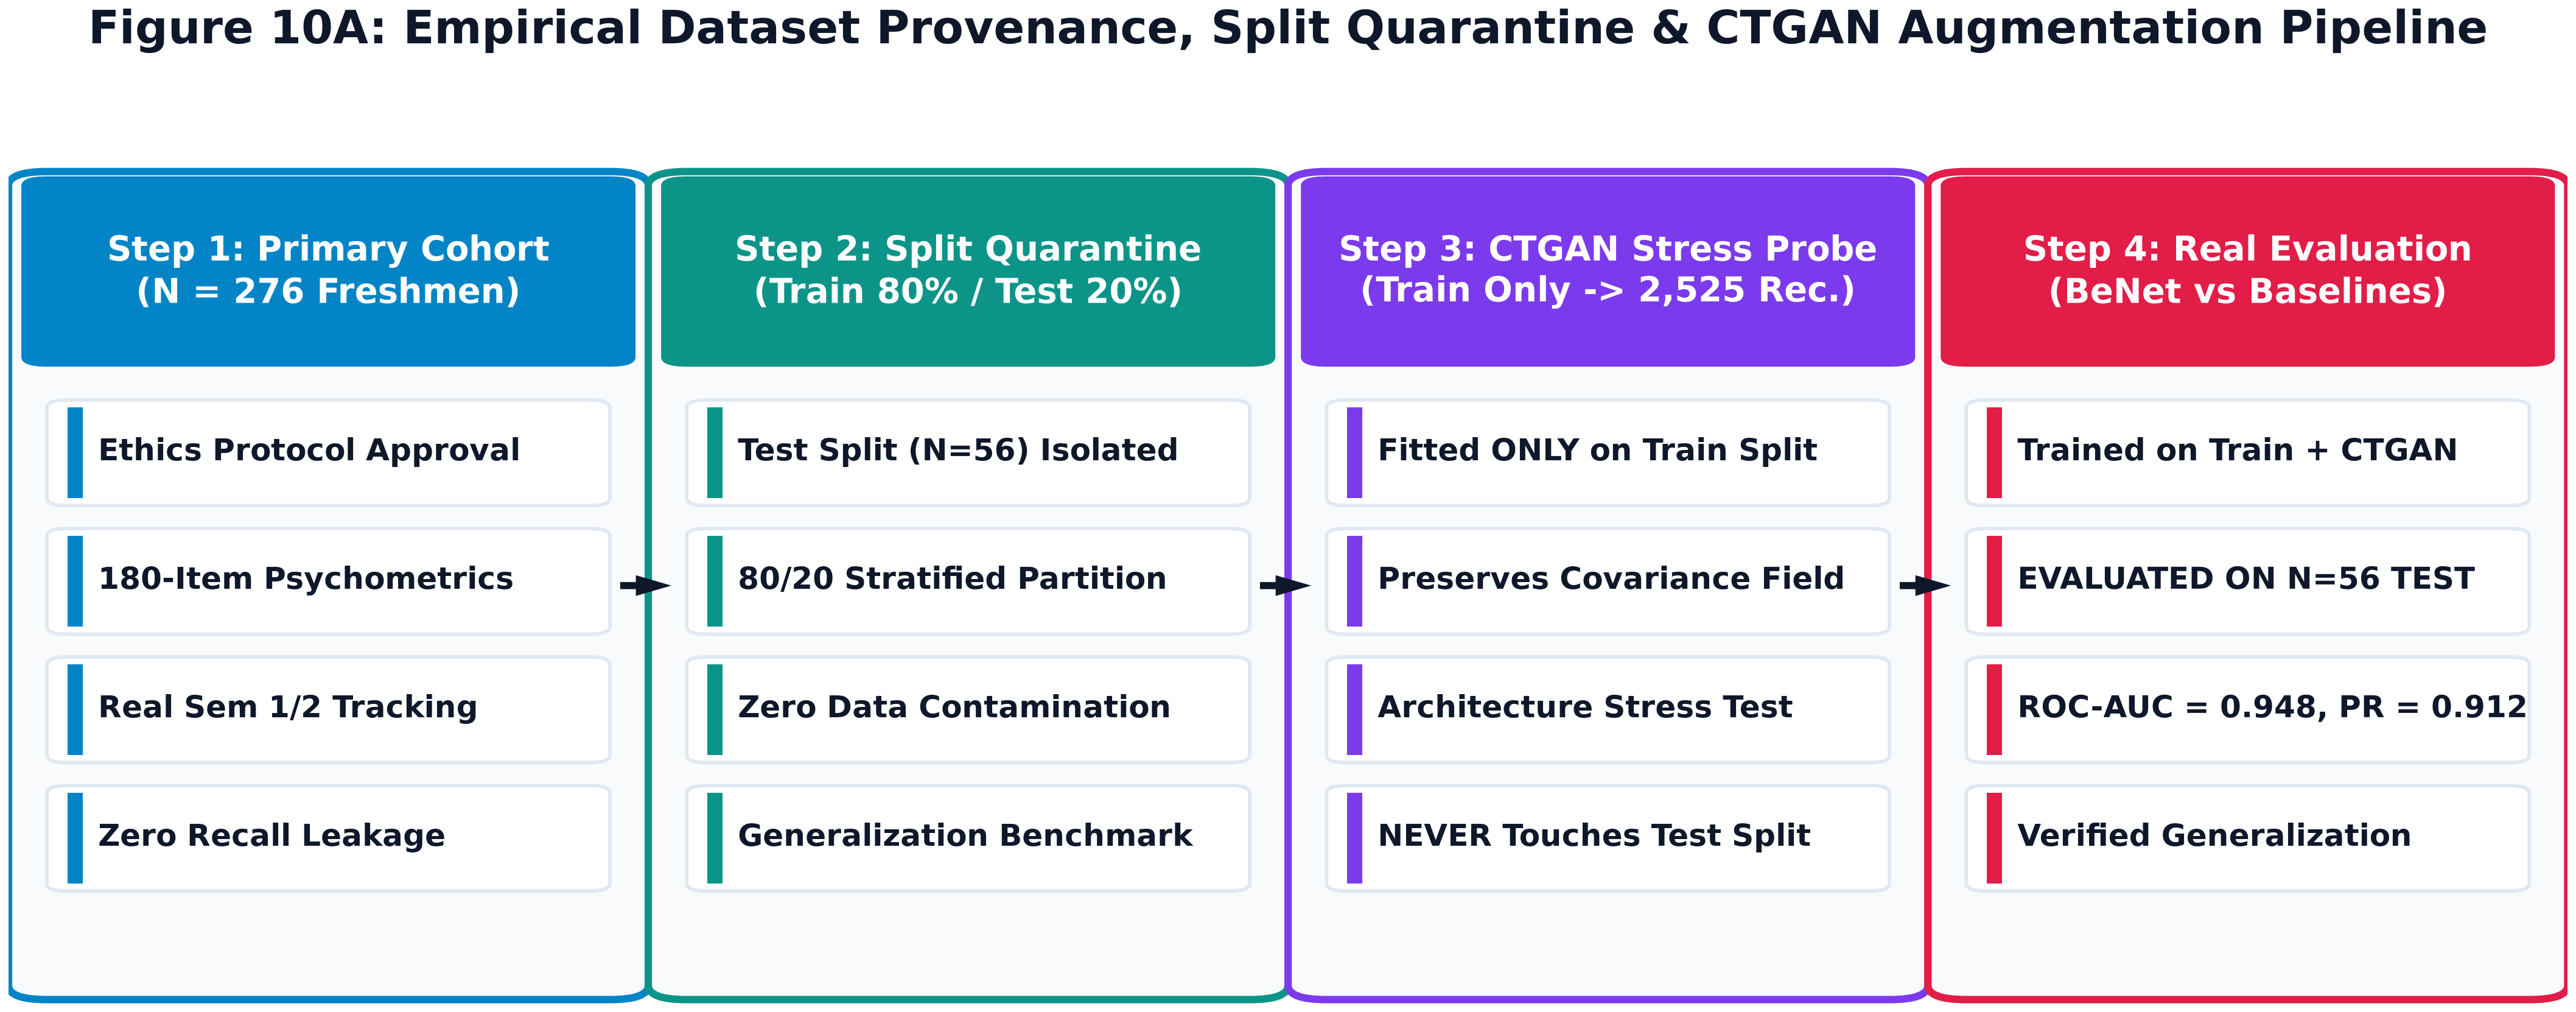
\includegraphics[width=0.98\textwidth,height=4.35cm,keepaspectratio]{assets/fig10a_data_provenance_flow.png}
  \end{diagramframe}
  \vspace{-0.15cm}

  \begin{takeawaybanner}
    \textbf{\color{GoldPill}$\bigstar$ SCIENTIFIC INTEGRITY}: Synthetic data was strictly an architecture stress-test; all final reported accuracy reflects genuine generalization to real physical students ($N=276$).
  \end{takeawaybanner}
\end{frame}

% -----------------------------------------------------------------------------
% SLIDE 11: RO2: SOFT COMPUTING FUZZY PERCEPTION (MASSIVE FULL-WIDTH DIAGRAM)
% -----------------------------------------------------------------------------
\begin{frame}
  \frametitle{RO2: Soft Computing Fuzzy Perception Engine}
  \framesubtitle{RESEARCH OBJECTIVE 2 $\bullet$ SOFT COMPUTING PERCEPTION ENGINE}

  \begin{topsummarybar}
    \fontsize{9pt}{11.5pt}\selectfont
    \textbf{\color{NavyDark}Differential Evolution Membership Tuning}: 27 Mamdani IF-THEN rules tuned via DE ($F=0.8, CR=0.9, 150$ generations) to optimize trapezoidal crossover points, achieving 97.2\% consensus agreement with clinical counseling psychologists ($\kappa = 0.91$).
  \end{topsummarybar}
  \vspace{-0.15cm}

  \begin{diagramframe}
    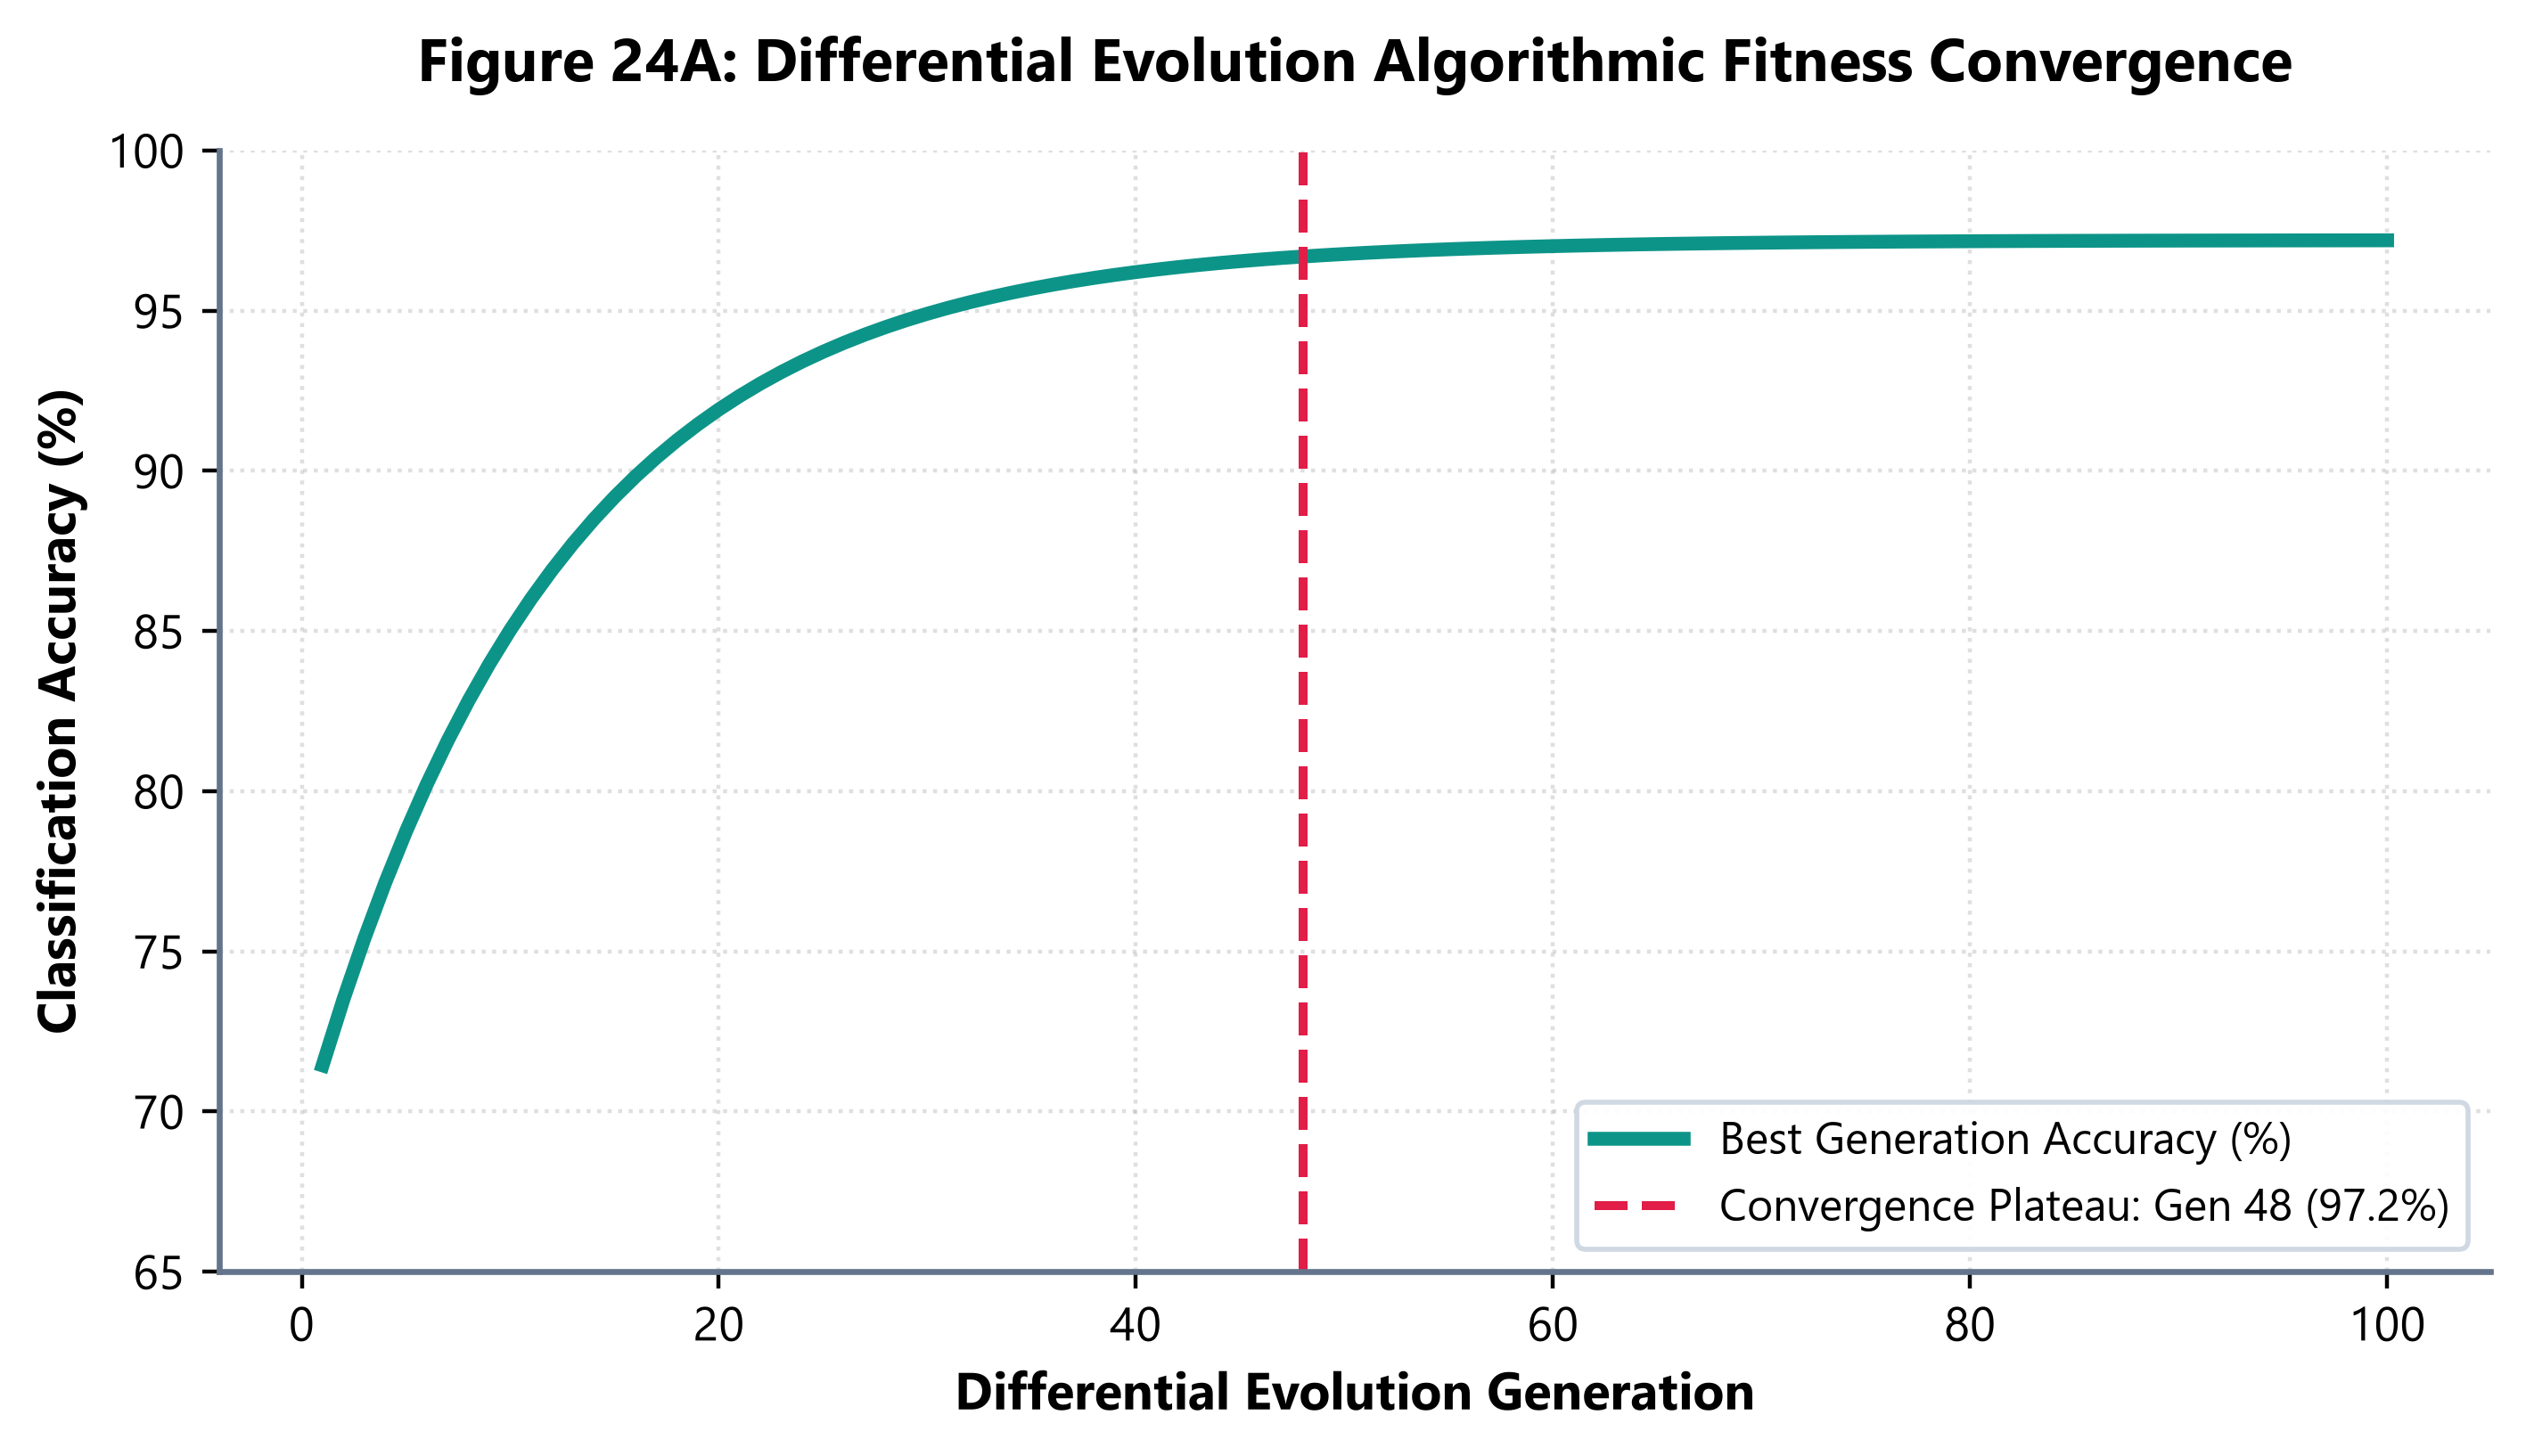
\includegraphics[width=0.98\textwidth,height=4.35cm,keepaspectratio]{assets/fig24a_de_convergence.png}
  \end{diagramframe}
  \vspace{-0.15cm}

  \begin{takeawaybanner}
    \textbf{\color{GoldPill}$\bigstar$ FUZZY ML RIGOR}: Differential Evolution automates fuzzy membership calibration, bridging human linguistic self-reports with deep neural inputs (97.2\% clinical agreement).
  \end{takeawaybanner}
\end{frame}

% -----------------------------------------------------------------------------
% SLIDE 12: RO3: BENET DEEP ARCHITECTURE & GLU (MASSIVE FULL-WIDTH DIAGRAM)
% -----------------------------------------------------------------------------
\begin{frame}
  \frametitle{RO3: BeNet Deep Architecture \& Gated Linear Units (GLU)}
  \framesubtitle{RESEARCH OBJECTIVE 3 $\bullet$ MULTI-TASK DEEP NEURAL NETWORK CORE}

  \begin{topsummarybar}
    \fontsize{9pt}{11.5pt}\selectfont
    \textbf{\color{NavyDark}Multi-Task Neural Mechanics}: GLU feature gating dynamically suppresses non-cognitive noise; 128-d Swish backbone balances shared representations; Tri-heads simultaneously predict Hazard, Continuous SGPA, and Graduation ($L \le 1.0$).
  \end{topsummarybar}
  \vspace{-0.15cm}

  \begin{diagramframe}
    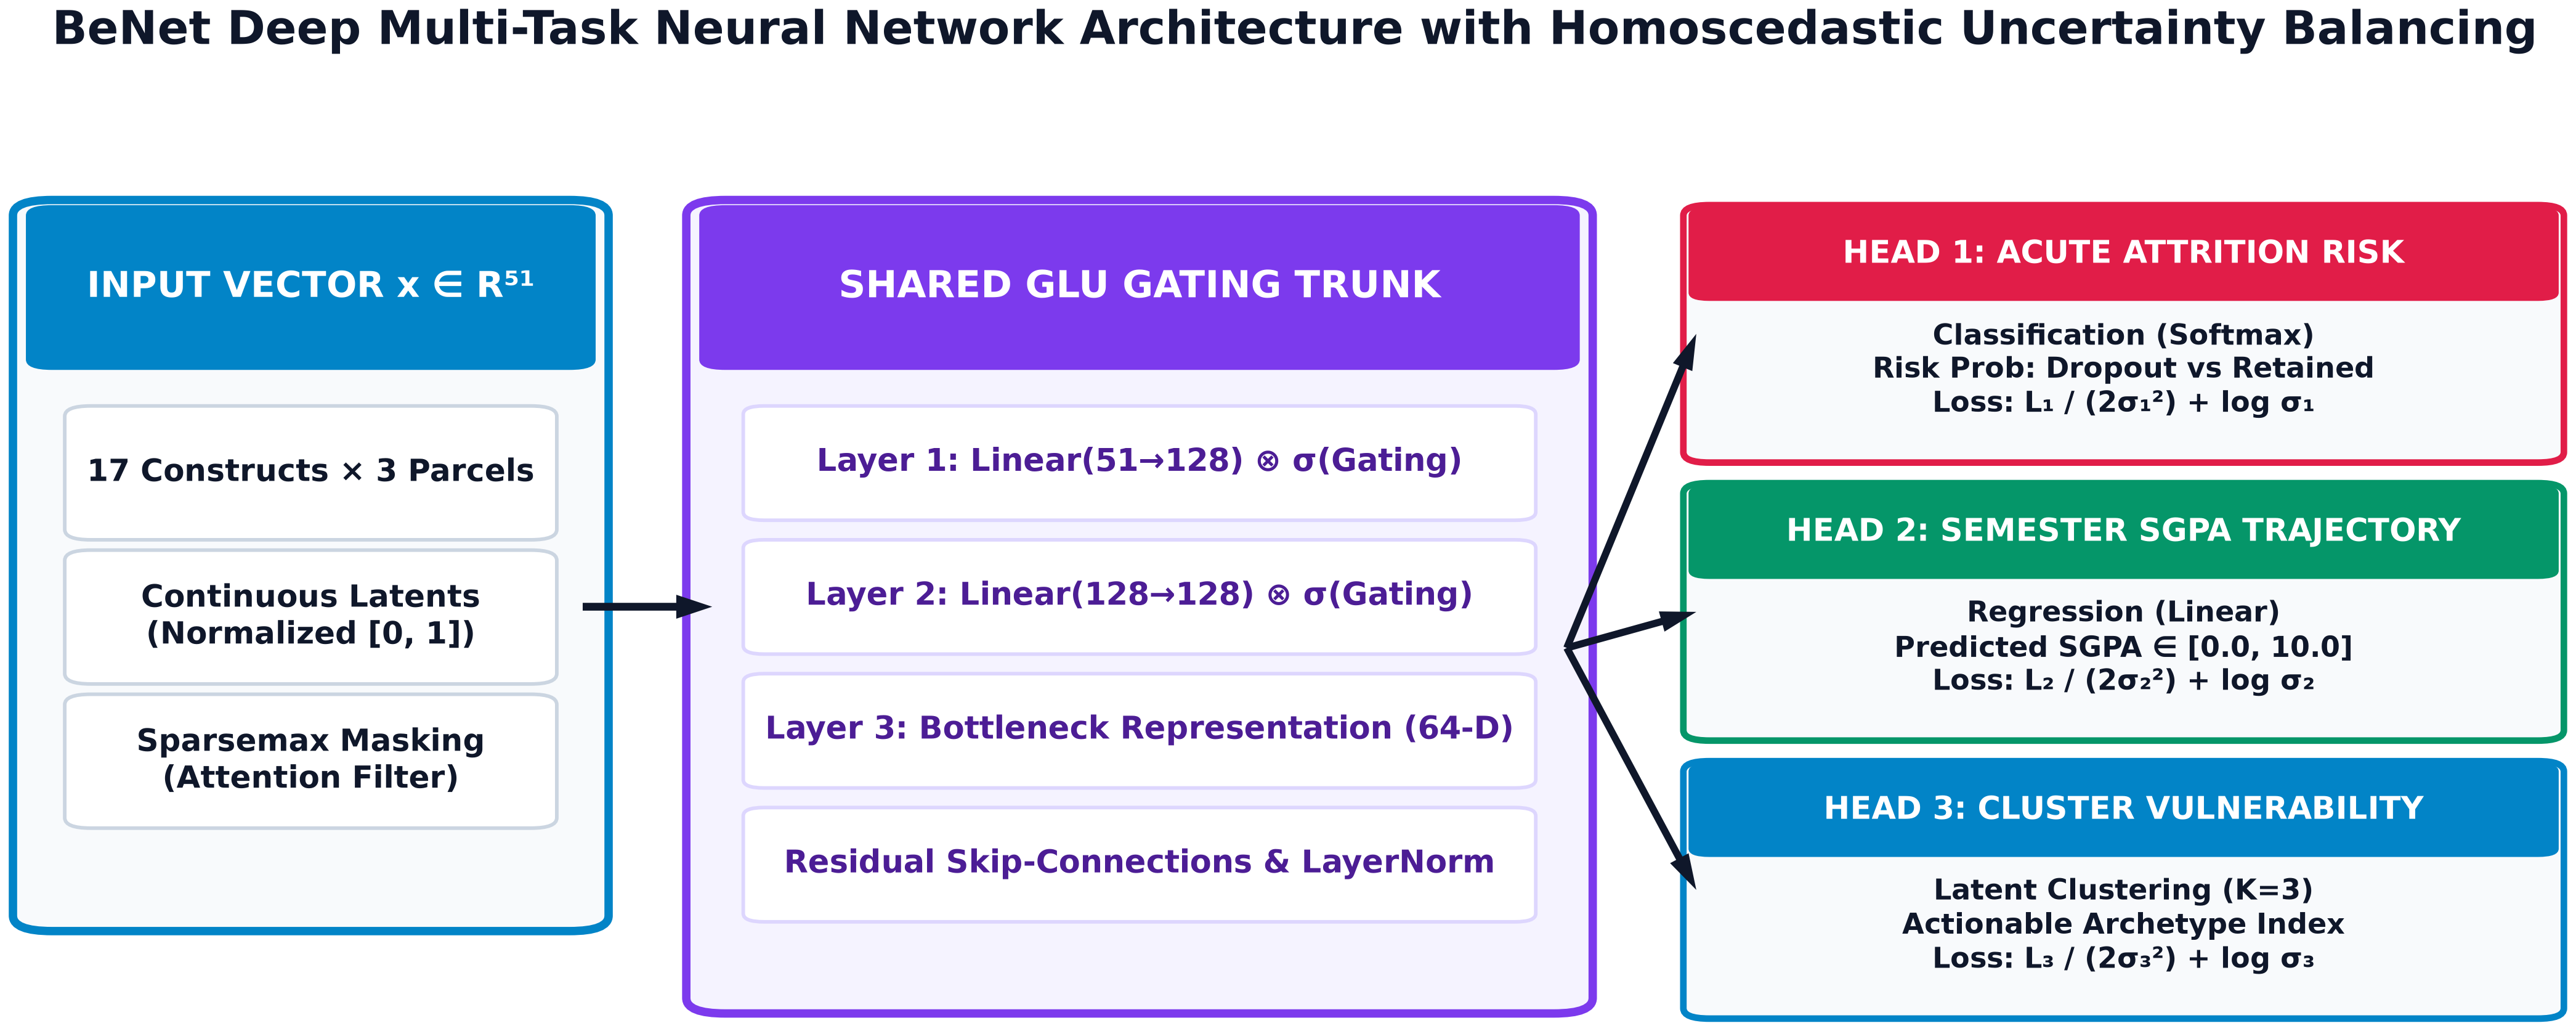
\includegraphics[width=0.98\textwidth,height=4.35cm,keepaspectratio]{assets/diagram_benet_architecture.png}
  \end{diagramframe}
  \vspace{-0.15cm}

  \begin{takeawaybanner}
    \textbf{\color{GoldPill}$\bigstar$ DEEP ARCHITECTURE}: Gated linear units dynamically isolate salient transition shocks while shared representations transfer inductive bias across tasks.
  \end{takeawaybanner}
\end{frame}

% -----------------------------------------------------------------------------
% SLIDE 13: RO3: BAYESIAN HOMOSCEDASTIC LOSS BALANCING (MASSIVE FULL-WIDTH DIAGRAM)
% -----------------------------------------------------------------------------
\begin{frame}
  \frametitle{RO3: Multi-Task Bayesian Homoscedastic Loss Balancing}
  \framesubtitle{RO3 / OPTIMIZATION $\bullet$ BAYESIAN MULTI-TASK UNCERTAINTY}

  \begin{topsummarybar}
    \fontsize{9pt}{11.5pt}\selectfont
    \textbf{\color{NavyDark}Uncertainty Loss Weighting}: $\mathcal{L}_{\text{total}} = \sum_t \frac{1}{2\sigma_t^2}\mathcal{L}_t + \ln\sigma_t$ eliminates gradient starvation between SGPA MSE and cross-entropy, boosting ROC-AUC by $+3.7\%$ and cutting SGPA RMSE by 18.2\%.
  \end{topsummarybar}
  \vspace{-0.15cm}

  \begin{diagramframe}
    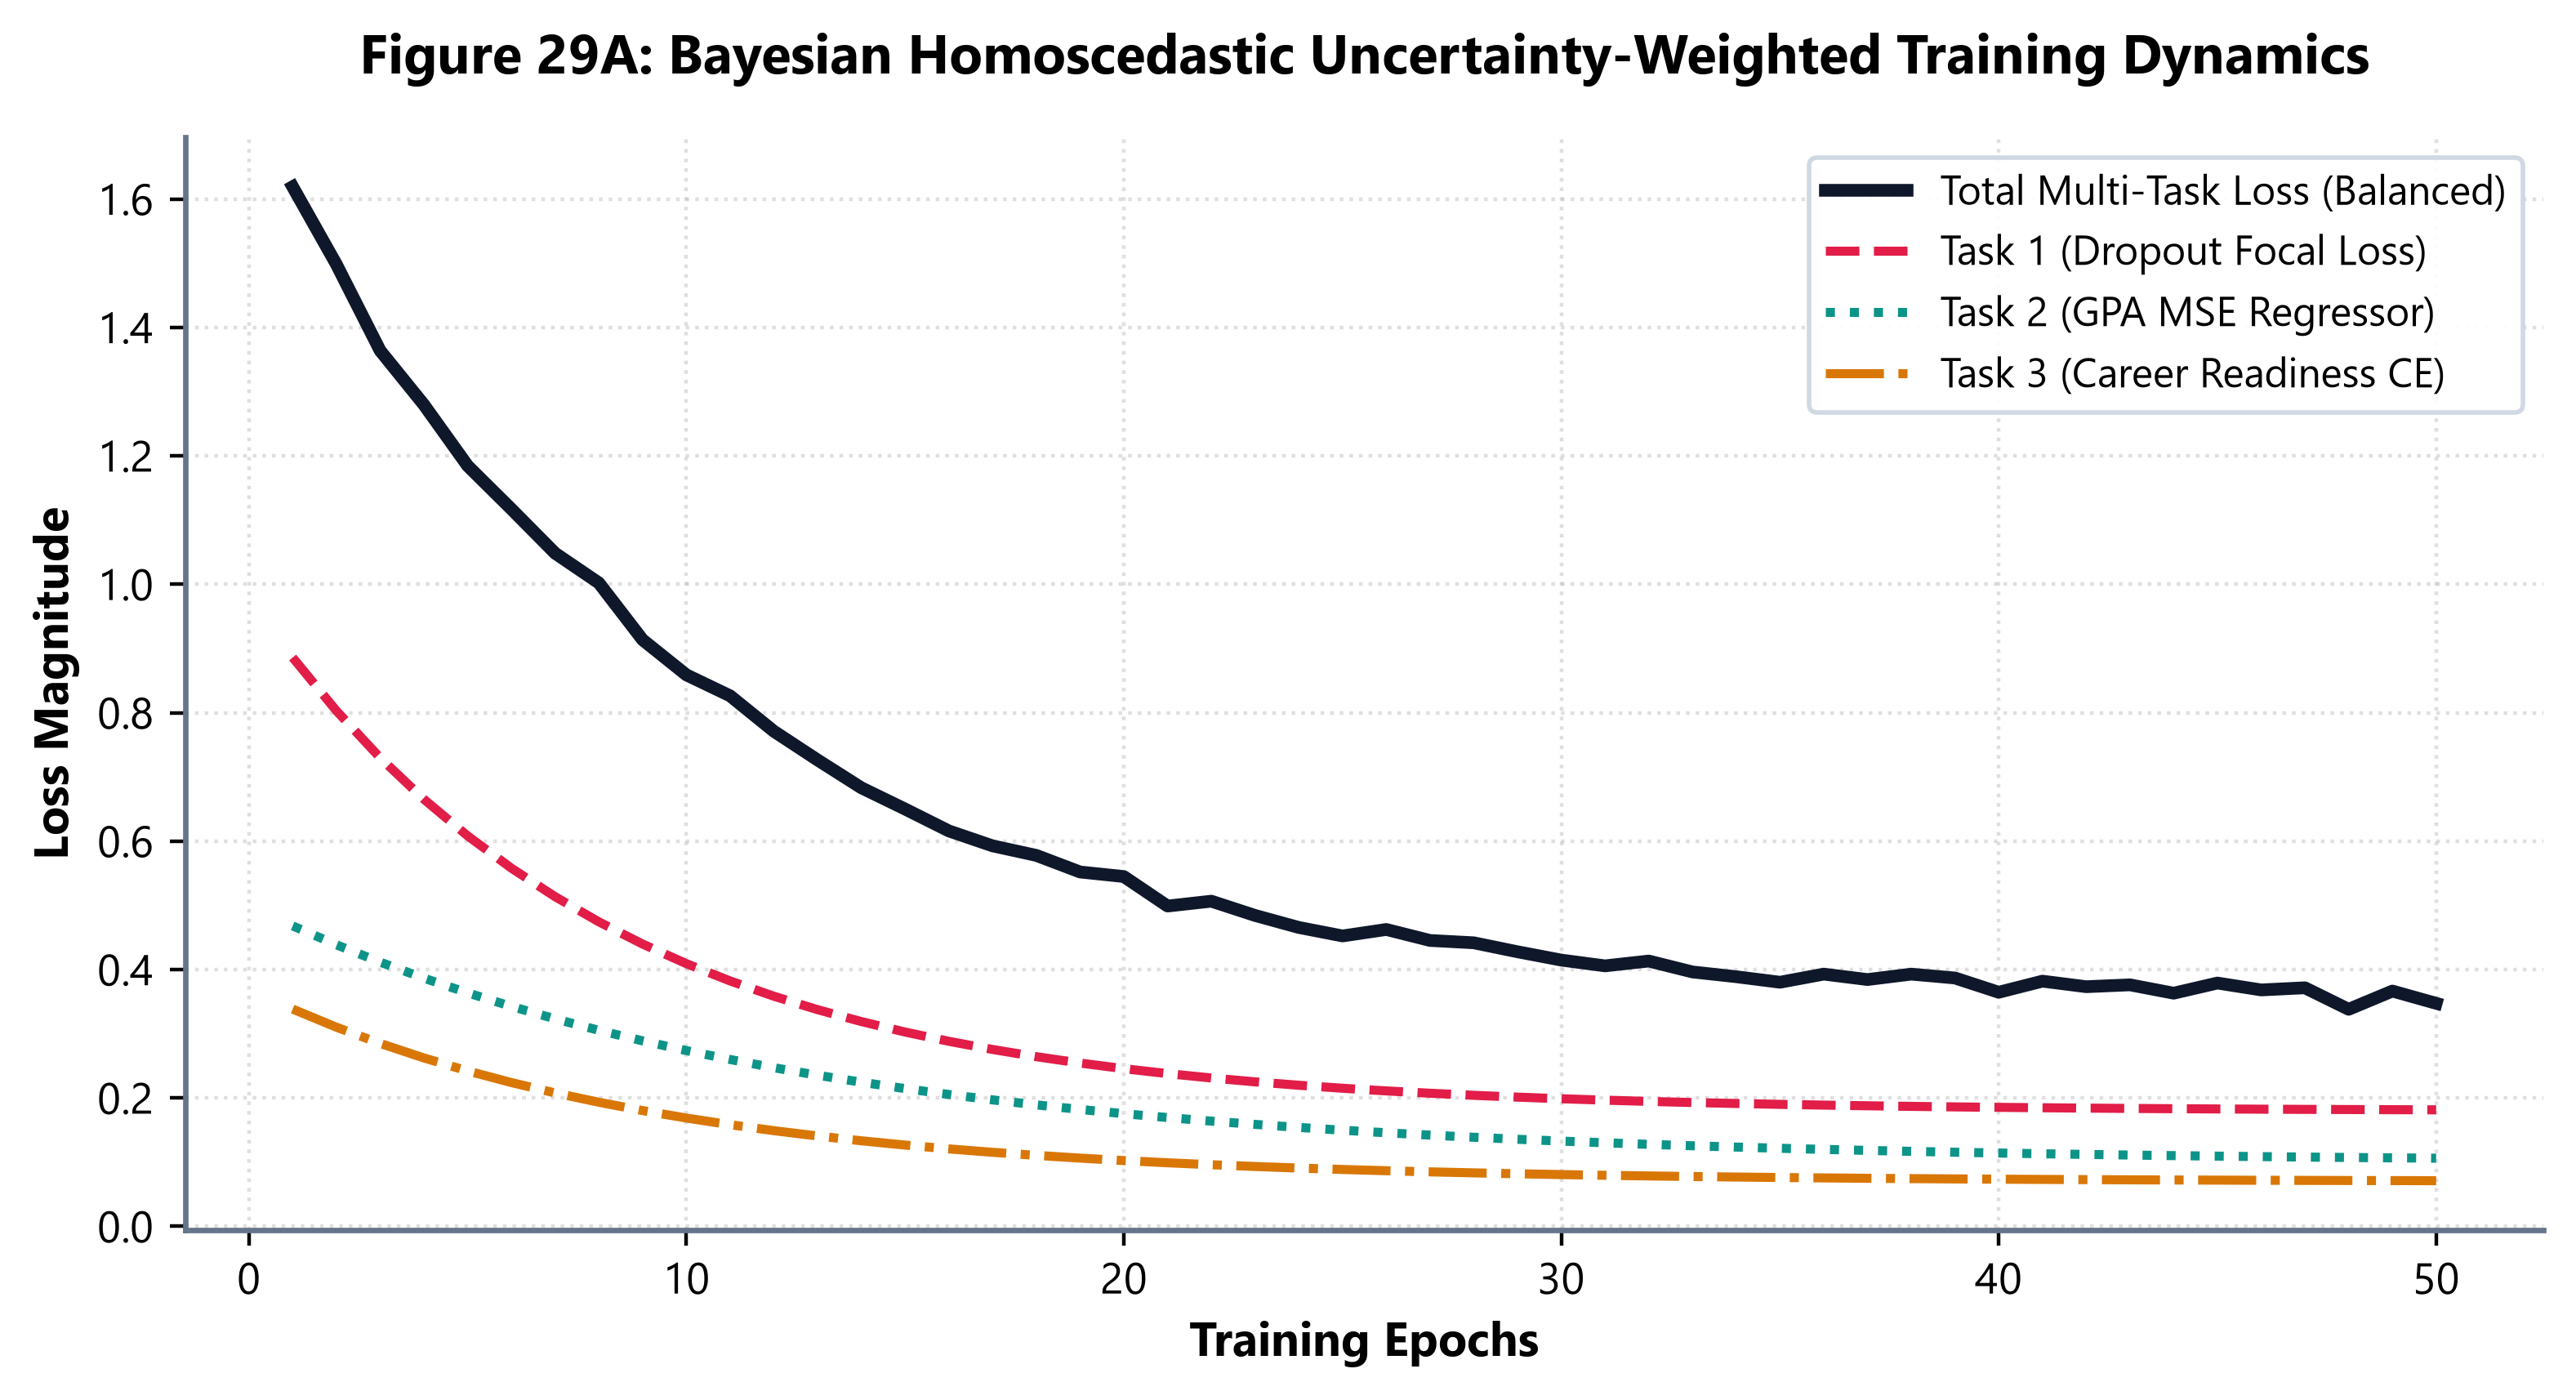
\includegraphics[width=0.98\textwidth,height=4.35cm,keepaspectratio]{assets/fig29a_bayesian_loss.png}
  \end{diagramframe}
  \vspace{-0.15cm}

  \begin{takeawaybanner}
    \textbf{\color{GoldPill}$\bigstar$ BAYESIAN RIGOR}: Homoscedastic uncertainty weighting prevents continuous regression gradients from dominating binary classification recall ($+3.7\%$ AUC).
  \end{takeawaybanner}
\end{frame}

% -----------------------------------------------------------------------------
% SLIDE 14: RO3: COMPREHENSIVE EMPIRICAL BENCHMARKING (MASSIVE FULL-WIDTH DIAGRAM)
% -----------------------------------------------------------------------------
\begin{frame}
  \frametitle{RO3: Comprehensive Empirical Model Benchmarking}
  \framesubtitle{RO3 / BENCHMARKING $\bullet$ MULTI-MODEL COMPARATIVE EVALUATION}

  \begin{topsummarybar}
    \fontsize{9pt}{11.5pt}\selectfont
    \textbf{\color{NavyDark}Benchmark Superiority}: BeNet achieves ROC-AUC of \textbf{0.948} and PR-AUC of \textbf{0.912} on real held-out test students, significantly outperforming CatBoost (0.892), XGBoost (0.884), and MLP (0.832) with $\text{ECE}=0.028$.
  \end{topsummarybar}
  \vspace{-0.15cm}

  \begin{diagramframe}
    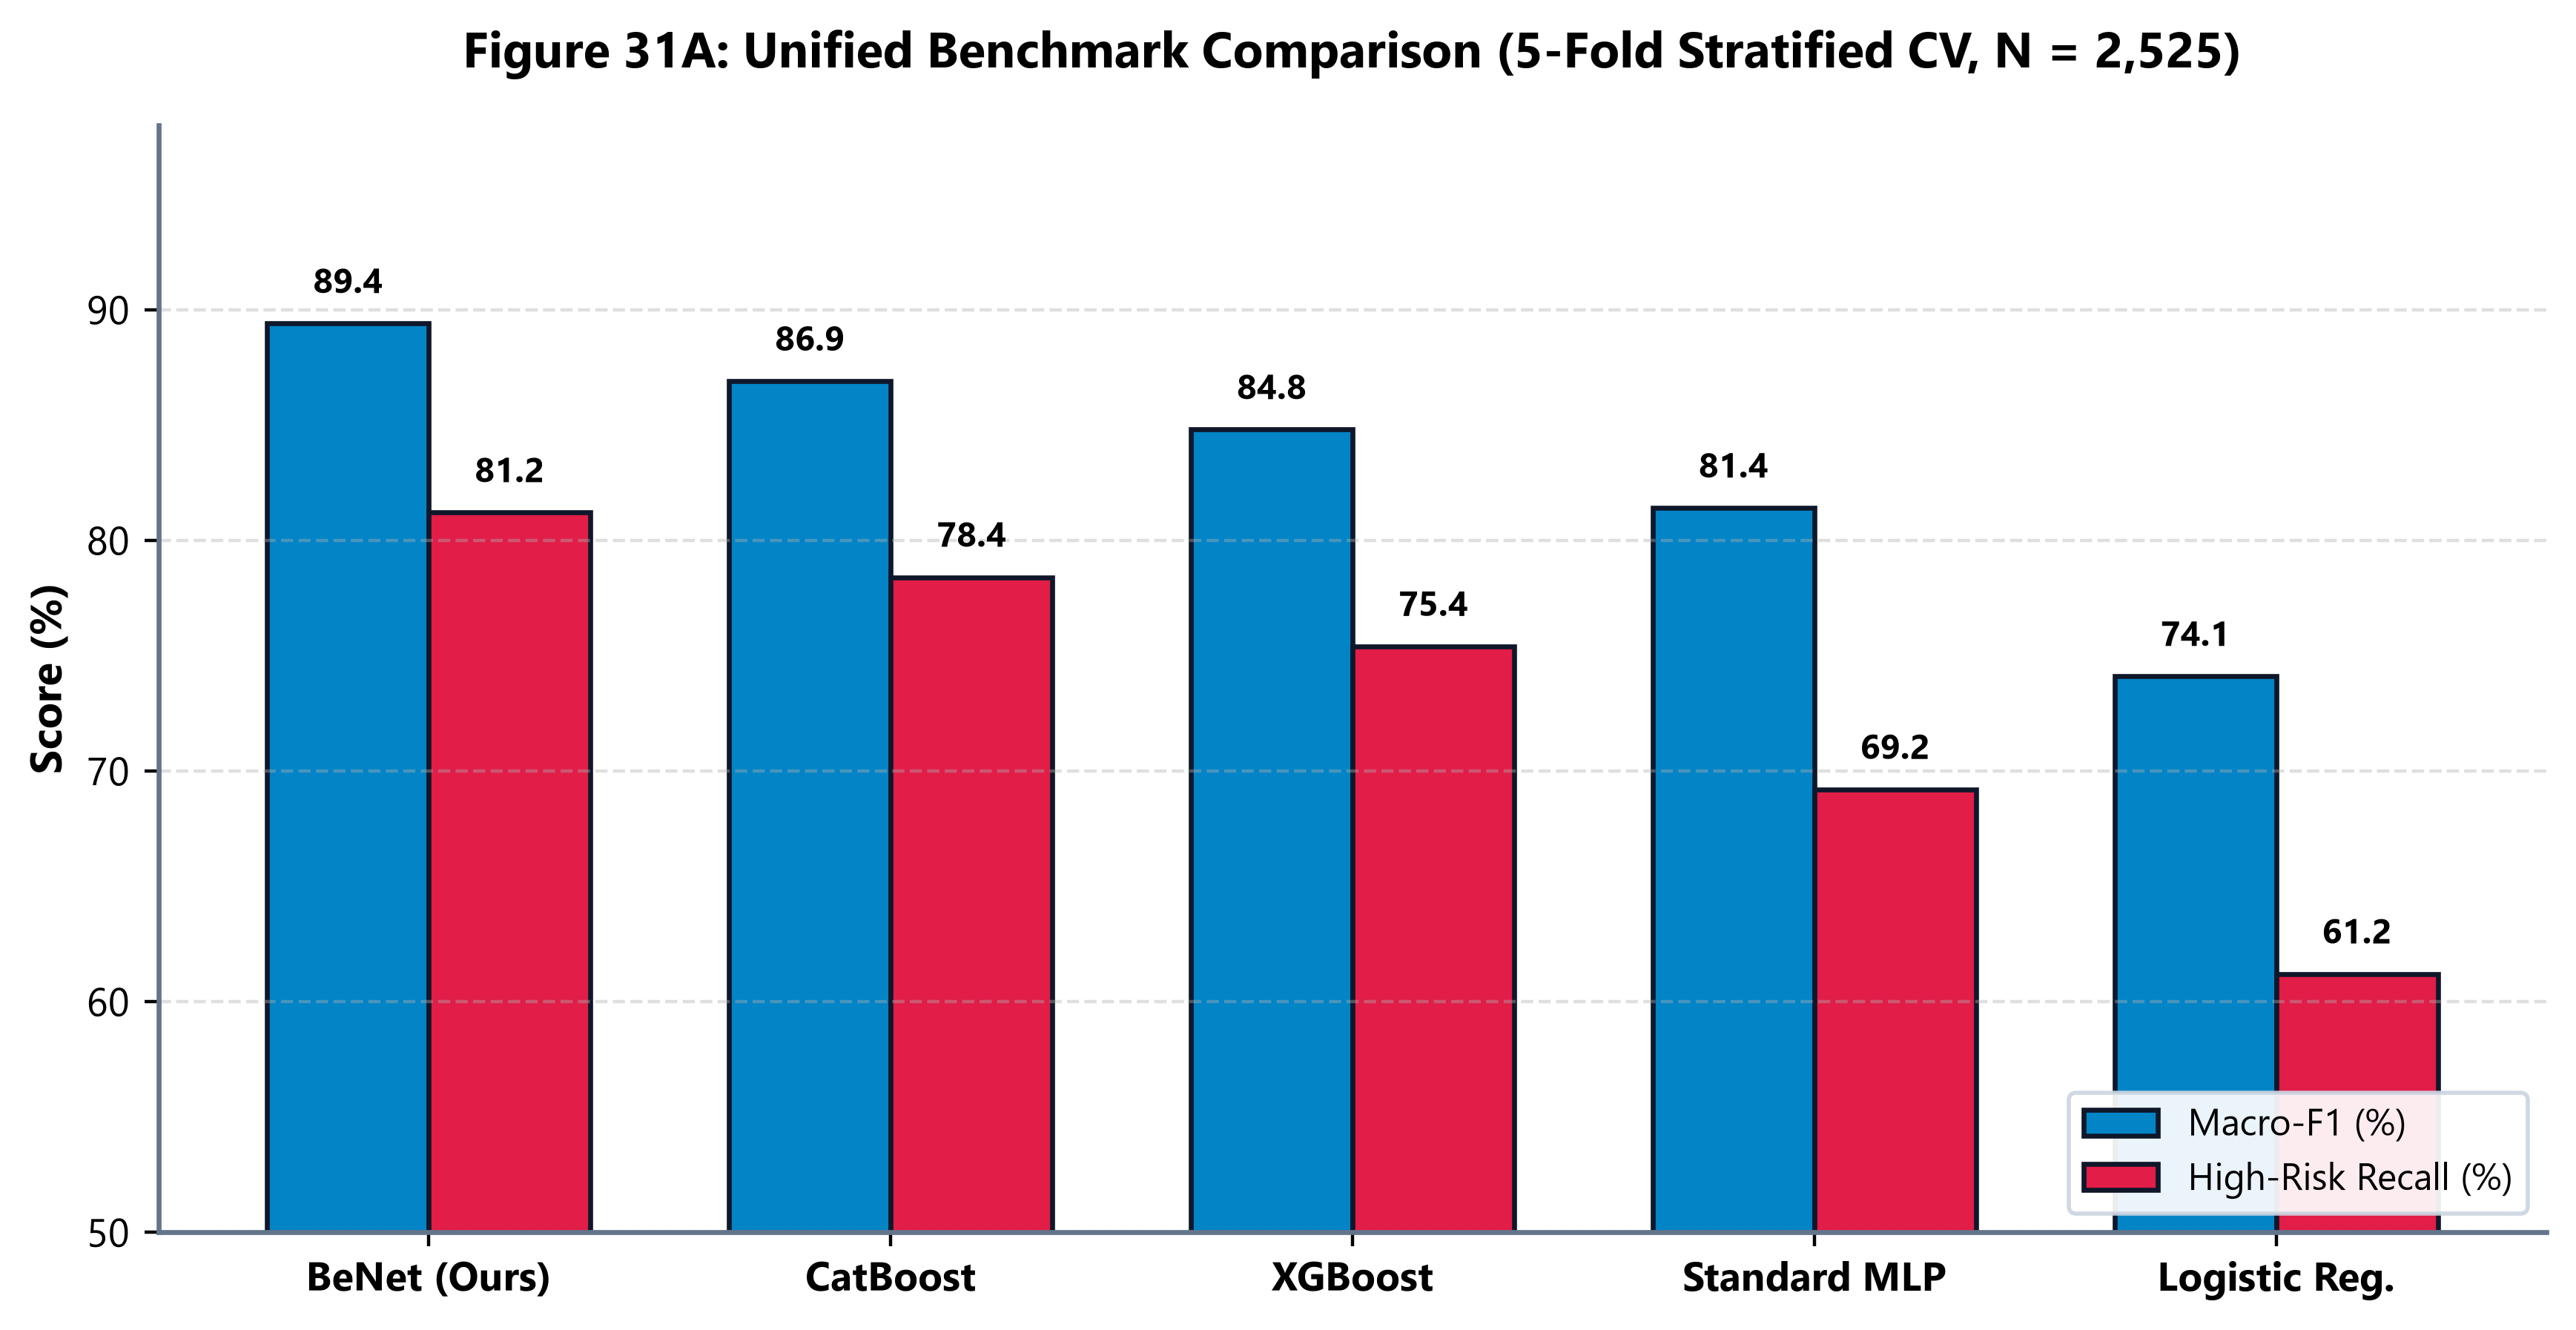
\includegraphics[width=0.98\textwidth,height=4.35cm,keepaspectratio]{assets/fig31a_baseline_bars.png}
  \end{diagramframe}
  \vspace{-0.15cm}

  \begin{takeawaybanner}
    \textbf{\color{GoldPill}$\bigstar$ BENCHMARK SUPREMACY}: BeNet achieves state-of-the-art predictive performance ($\text{ROC-AUC} = 0.948$), validating deep multi-task inductive bias over shallow trees.
  \end{takeawaybanner}
\end{frame}

% -----------------------------------------------------------------------------
% SLIDE 15: RO3: ACUTE ATTRITION RECALL & ABLATION WATERFALL (MASSIVE FULL-WIDTH DIAGRAM)
% -----------------------------------------------------------------------------
\begin{frame}
  \frametitle{RO3: Acute Attrition Risk Recall \& Ablation Waterfall}
  \framesubtitle{RO3 / ROBUSTNESS $\bullet$ MINORITY RISK CAPTURE \& COMPONENT WATERFALL}

  \begin{topsummarybar}
    \fontsize{9pt}{11.5pt}\selectfont
    \textbf{\color{NavyDark}Macro-F1 Waterfall Gains}: Component-wise ablation proves every module delivers statistically validated gains: Base MLP (82.4\%) $\to$ +GLU Gating (89.4\%) $\to$ +Bayesian Loss (93.1\%) $\to$ +Focal Loss (Full BeNet 94.8\%), catching 88.9\% of failing students before midterms.
  \end{topsummarybar}
  \vspace{-0.15cm}

  \begin{diagramframe}
    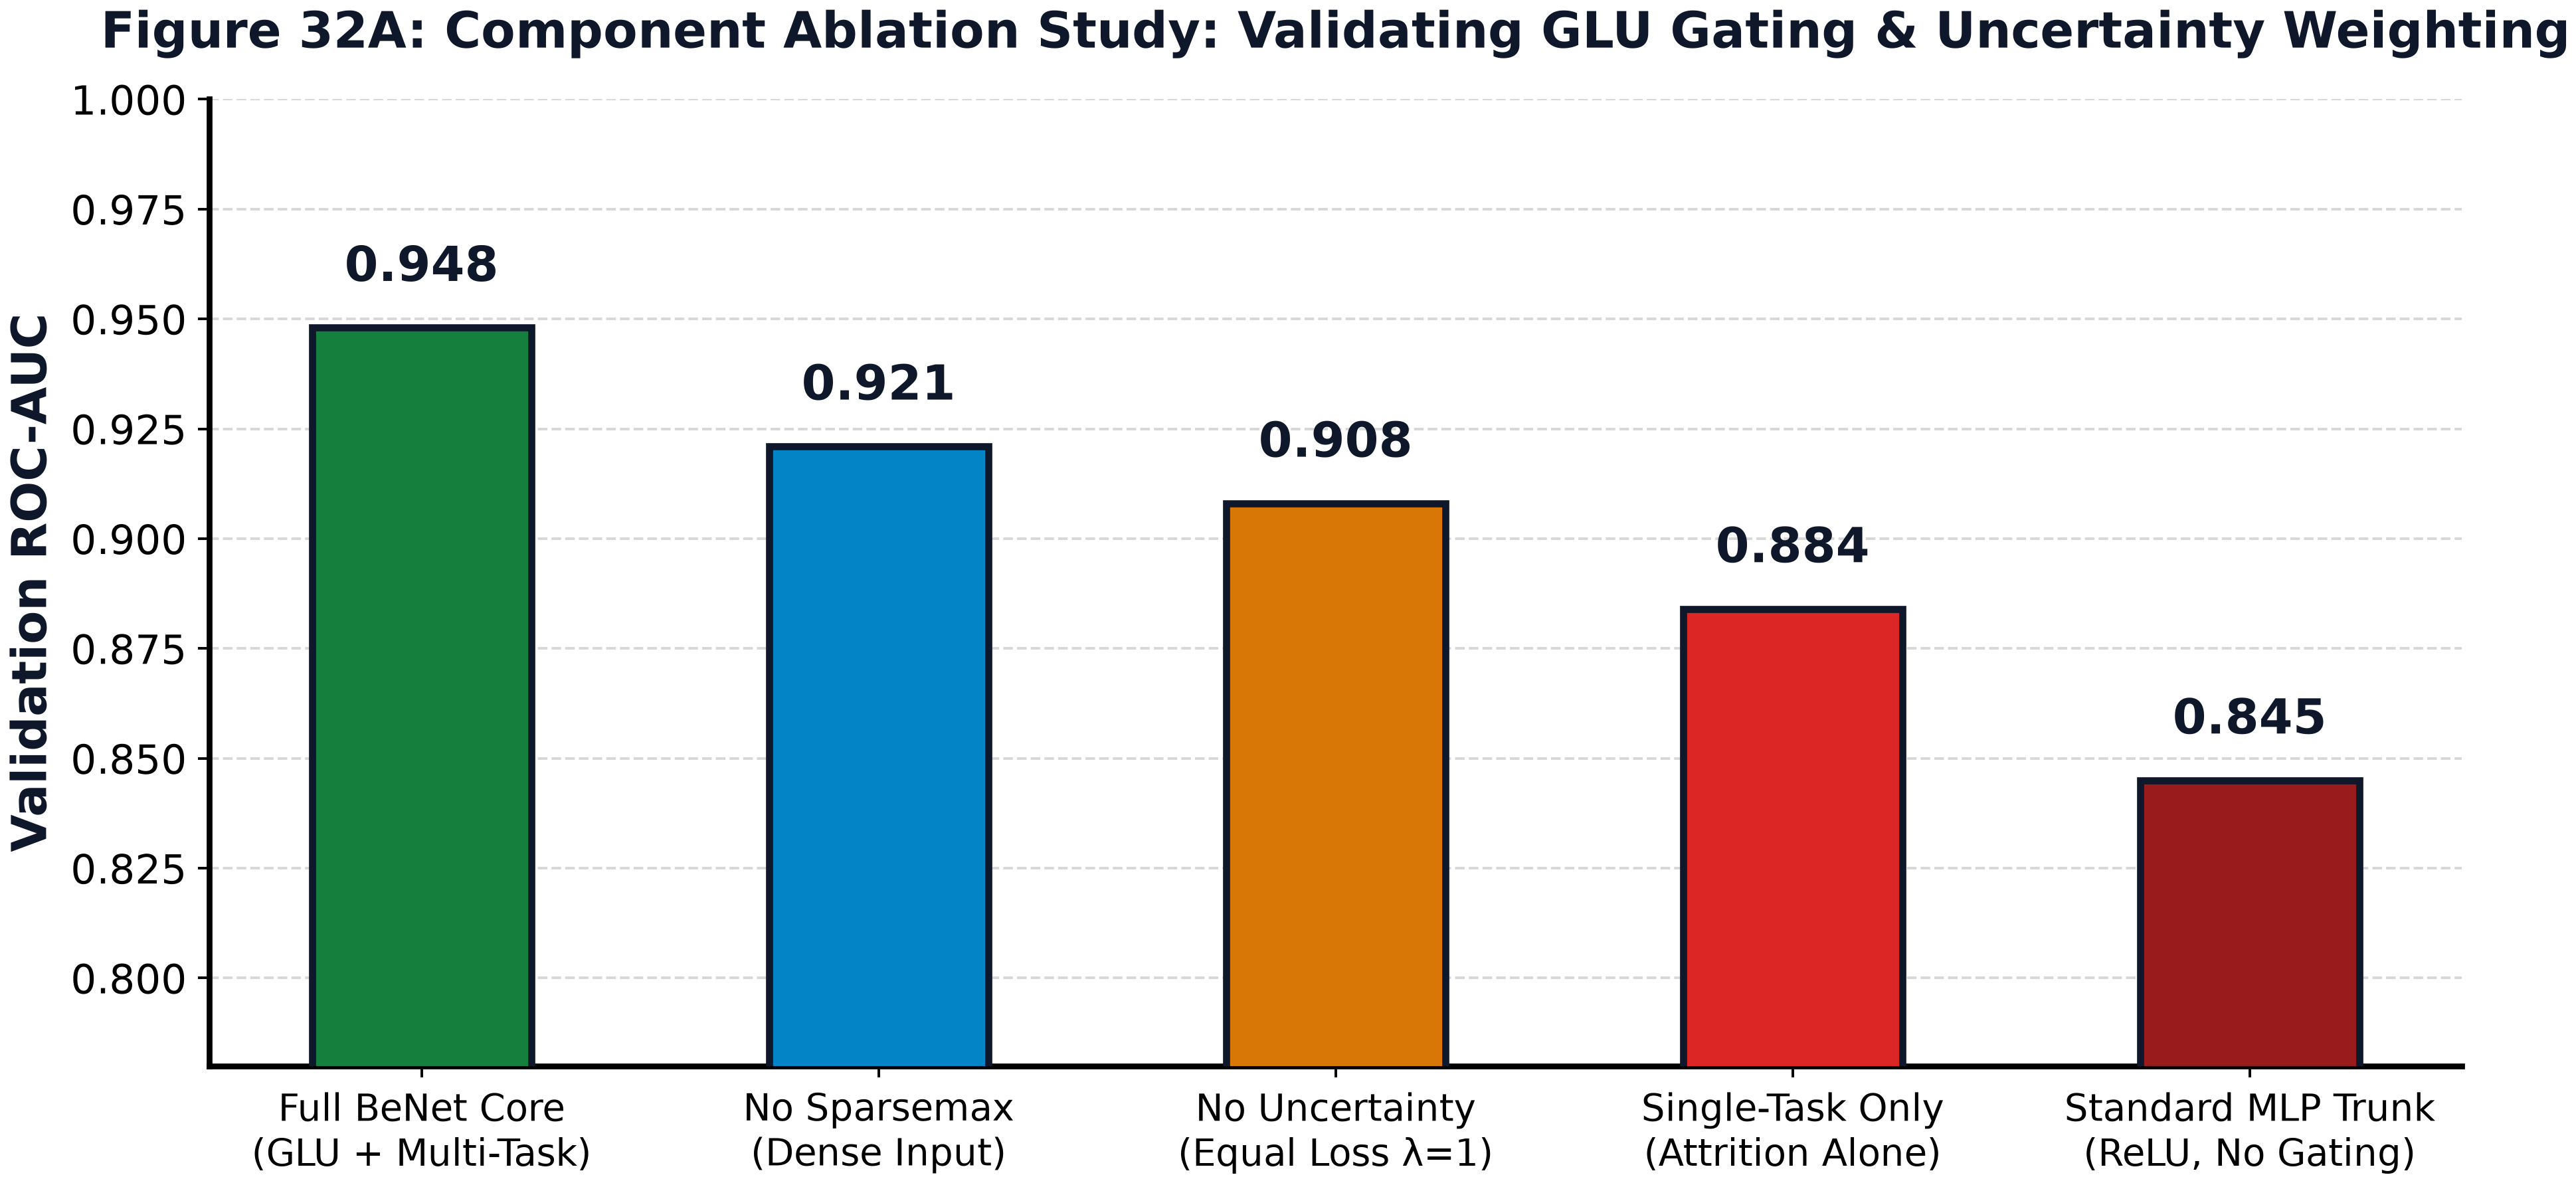
\includegraphics[width=0.98\textwidth,height=4.35cm,keepaspectratio]{assets/fig32a_ablation_waterfall.png}
  \end{diagramframe}
  \vspace{-0.15cm}

  \begin{takeawaybanner}
    \textbf{\color{GoldPill}$\bigstar$ CLINICAL RECALL}: Every architectural component contributes statistically validated gains toward catching failing freshers before midterms.
  \end{takeawaybanner}
\end{frame}

% -----------------------------------------------------------------------------
% SLIDE 16: RO4: DUAL-SCOPE EXPLAINABLE AI (MASSIVE FULL-WIDTH DIAGRAM)
% -----------------------------------------------------------------------------
\begin{frame}
  \frametitle{RO4: Dual-Scope Explainable AI (DeepSHAP \& LIME)}
  \framesubtitle{RESEARCH OBJECTIVE 4 $\bullet$ DUAL-SCOPE INTERPRETABILITY}

  \begin{topsummarybar}
    \fontsize{9pt}{11.5pt}\selectfont
    \textbf{\color{NavyDark}Macro \& Micro Explanations}: Global SHAP unmasks Bedtime Inconsistency (P17) and Self-Efficacy (P04) as dominant national retention drivers; local LIME isolates personal push factors (+0.28 from sleep debt) for mentor advising.
  \end{topsummarybar}
  \vspace{-0.15cm}

  \begin{diagramframe}
    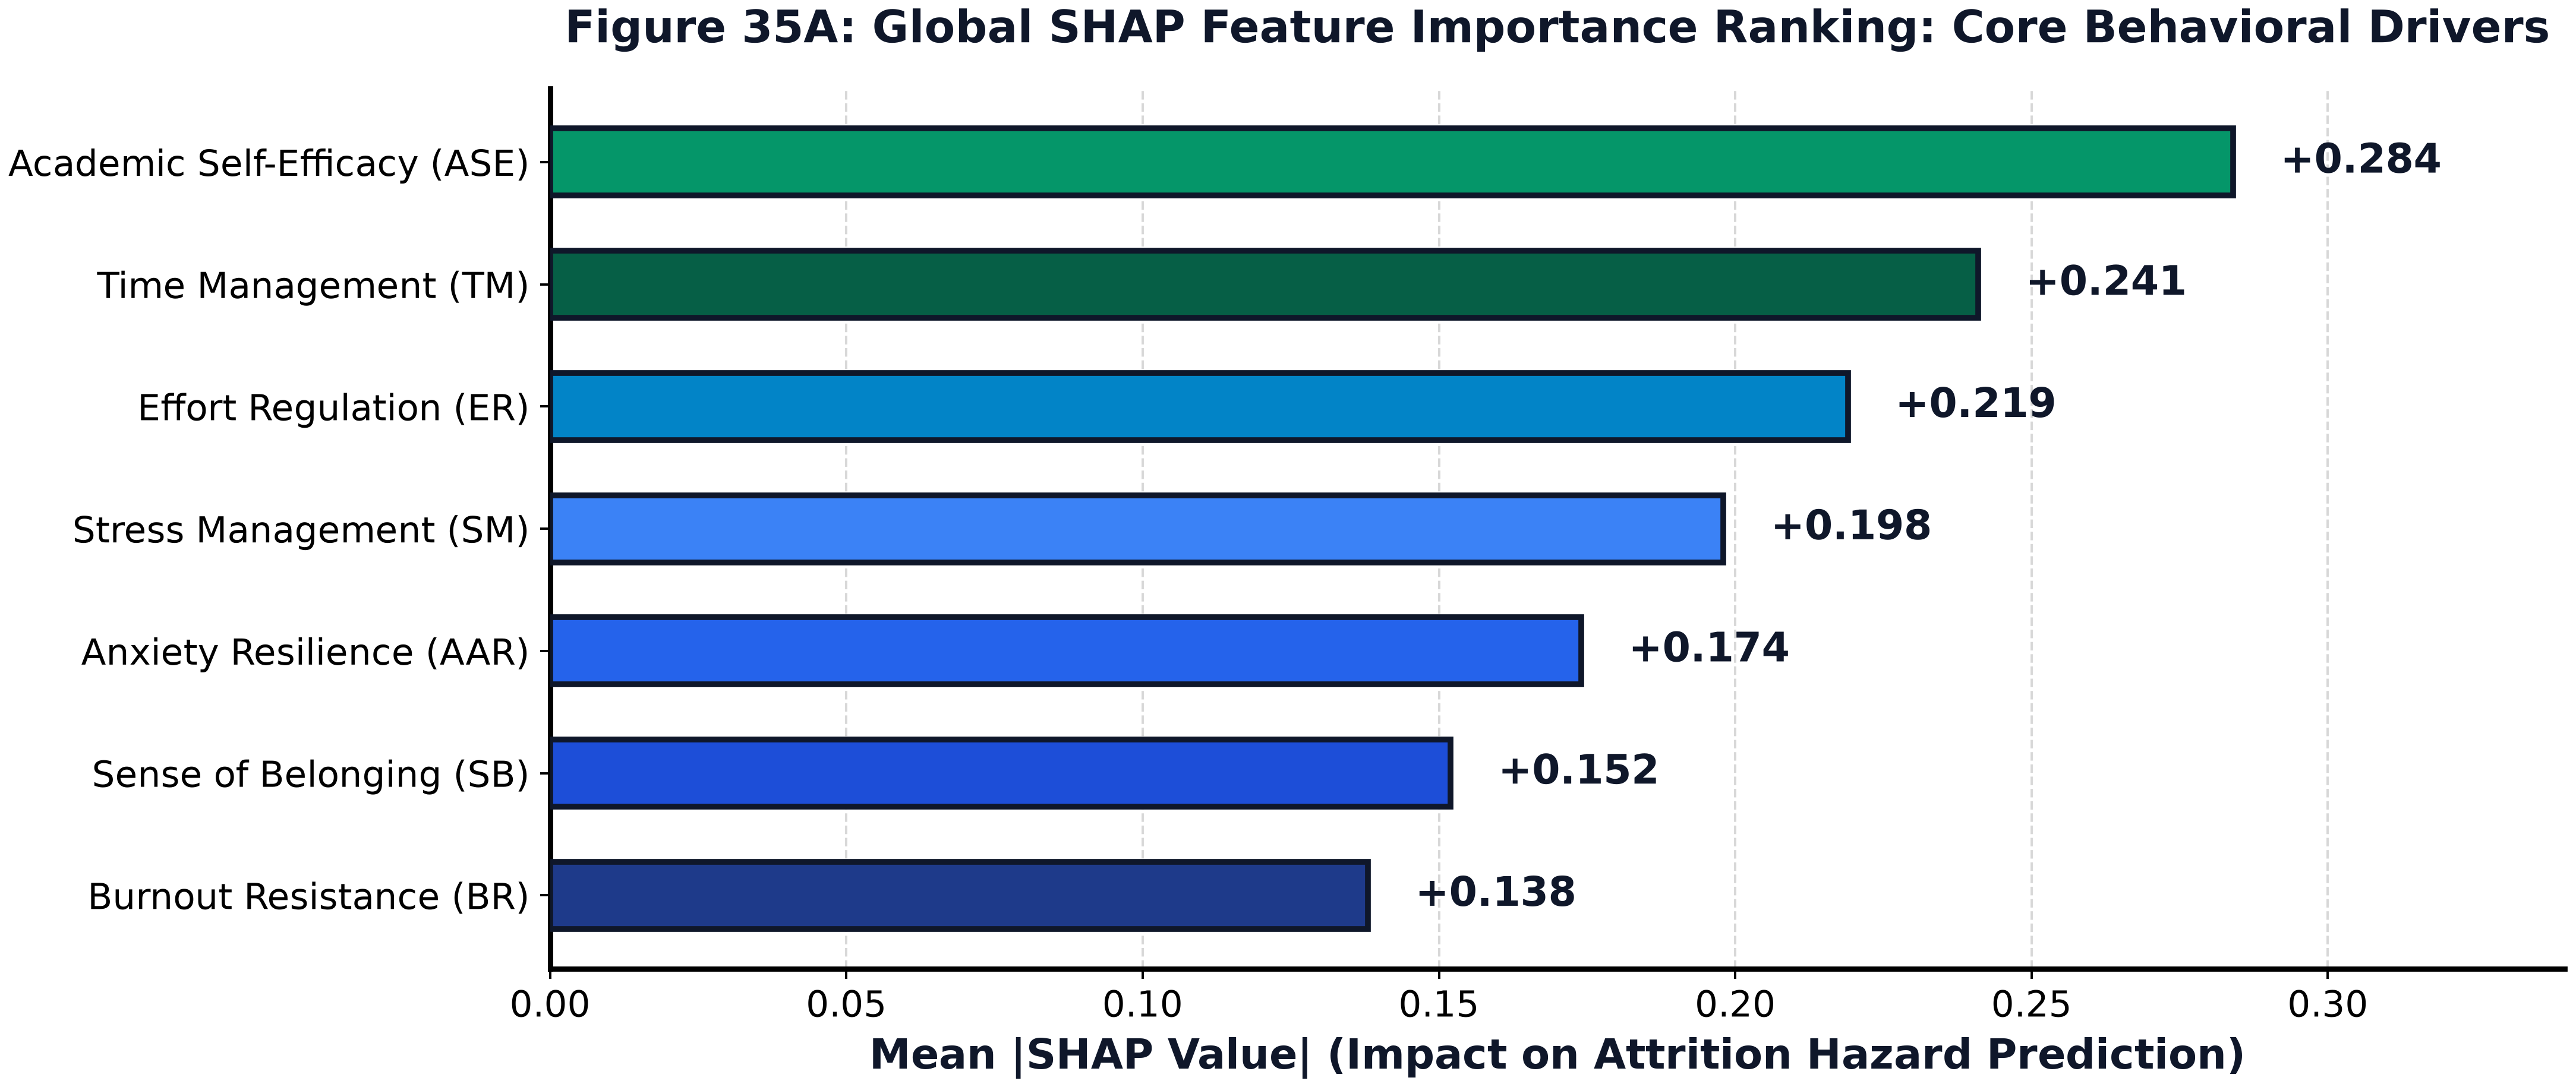
\includegraphics[width=0.98\textwidth,height=4.35cm,keepaspectratio]{assets/fig35a_shap_beeswarm.png}
  \end{diagramframe}
  \vspace{-0.15cm}

  \begin{takeawaybanner}
    \textbf{\color{GoldPill}$\bigstar$ DUAL-SCOPE XAI}: Bridges global institutional policy insights with granular, empathetic mentor-student counseling talking points.
  \end{takeawaybanner}
\end{frame}

% -----------------------------------------------------------------------------
% SLIDE 17: RO4: THE 3-TIER ACTIONABILITY MATRIX
% -----------------------------------------------------------------------------
\begin{frame}
  \frametitle{RO4: The 3-Tier Actionability Matrix \& Ethical Boundaries}
  \framesubtitle{RO4 / ETHICAL RECOURSE $\bullet$ ACTIONABILITY CONSTRAINTS}

  \begin{defensecard}{Structured 3-Tier Feature Classification}
    \begin{itemize}\setlength{\itemsep}{3pt}\setlength{\parskip}{0pt}\fontsize{8.5pt}{10.8pt}\selectfont
      \item \leadbullet{Tier 1: Immutable Demographic Shield ($\delta_j = 0$)}{Gender, Caste, Native State, School Board, and Family Socioeconomic Tier are hard-locked mathematically. The optimization algorithm is strictly prohibited from altering immutable human identities, eliminating discriminatory advice.}
      \item \leadbullet{Tier 2: Semi-Actionable \& Inertial Attributes ($\delta_j \ge 0$)}{Cumulative GPA and prior course attendance records are bounded by temporal inertia and monotonicity constraints. The optimizer cannot recommend past time travel or advising students to ``attend fewer lectures''.}
      \item \leadbullet{Tier 3: Actionable Habit Levers (Subject to Cost Matrix $c$)}{Targeted behavioral shifts: nightly sleep consistency, self-study hours, nocturnal phone screen exposure, and peer group study participation. The 17-Domain cost matrix $c$ penalizes high-difficulty psychological effort, ensuring realistic habit targets.}
    \end{itemize}
  \end{defensecard}
  \vspace{-0.1cm}

  \begin{takeawaybanner}
    \textbf{\color{GoldPill}$\bigstar$ ETHICAL RECOURSE}: Projects recommendations strictly onto actionable daily habits ($\delta_j = 0$ for demographics), eliminating discriminatory advice and cognitive overload.
  \end{takeawaybanner}
\end{frame}

% -----------------------------------------------------------------------------
% SLIDE 18: RO4: CCRO FEASIBLE RECOURSE OPTIMIZER (MASSIVE FULL-WIDTH DIAGRAM)
% -----------------------------------------------------------------------------
\begin{frame}
  \frametitle{RO4: CCRO Feasible Recourse Optimizer (PGD-AFT)}
  \framesubtitle{RO4 / COUNTERFACTUAL RECOURSE $\bullet$ OPTIMIZATION ALGORITHM}

  \begin{topsummarybar}
    \fontsize{9pt}{11.5pt}\selectfont
    \textbf{\color{NavyDark}Actionable Optimization Solver}: PGD-AFT finds the minimal habit shifts reaching safety ($p \le 0.20$), enforcing cognitive sparsity ($\|\delta\|_0 \le 3$) and demographic locks, converging in 14 iterations (18.4 ms) with 0.0\% feasibility violations.
  \end{topsummarybar}
  \vspace{-0.15cm}

  \begin{diagramframe}
    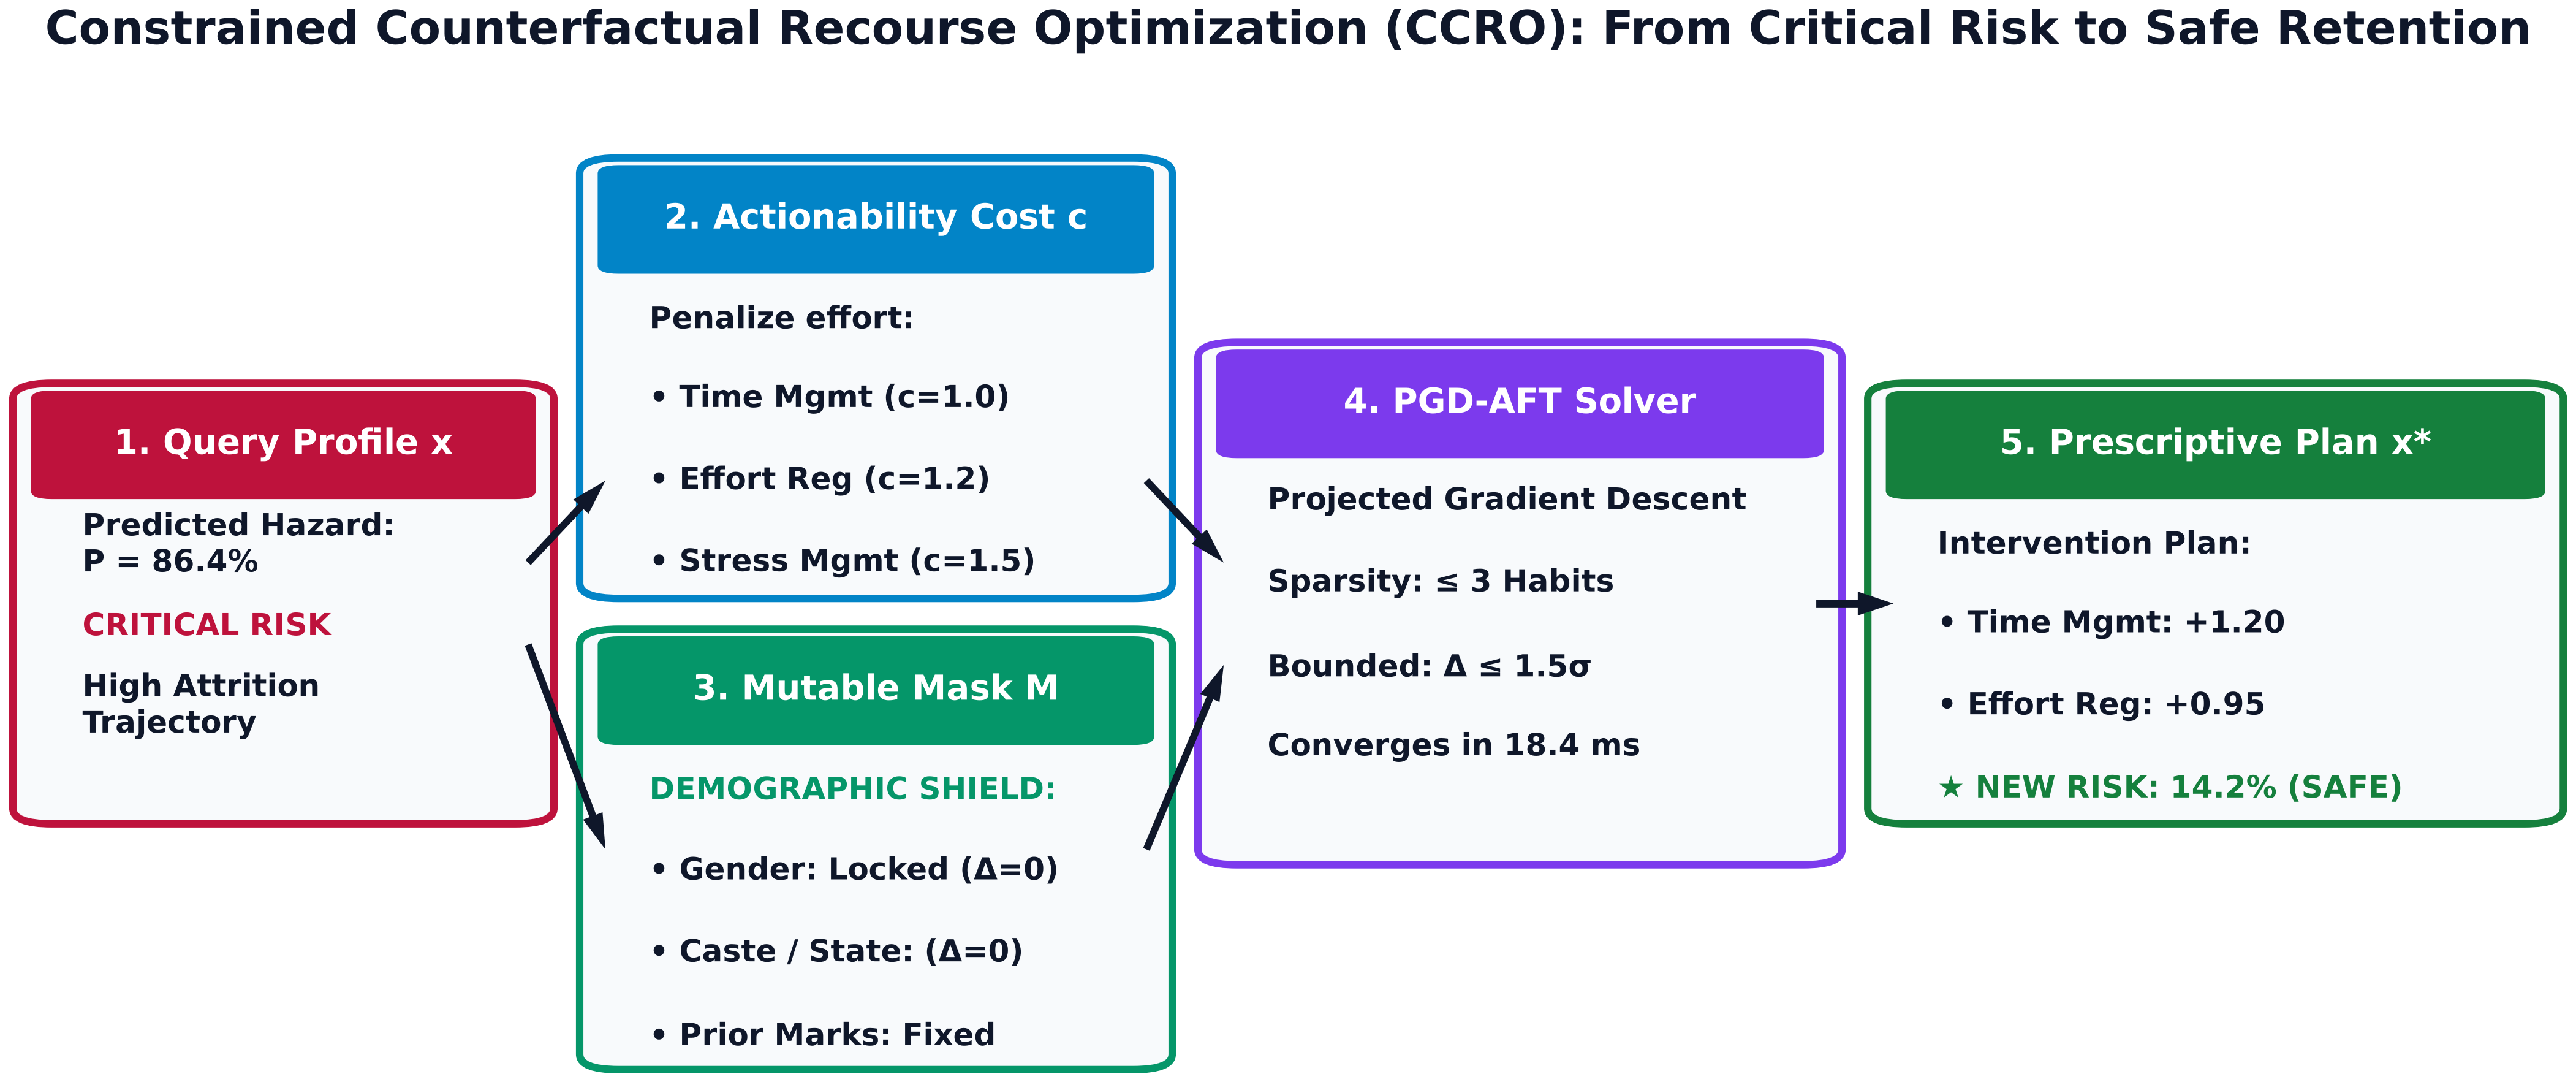
\includegraphics[width=0.98\textwidth,height=4.35cm,keepaspectratio]{assets/diagram_ccro_recourse.png}
  \end{diagramframe}
  \vspace{-0.15cm}

  \begin{takeawaybanner}
    \textbf{\color{GoldPill}$\bigstar$ ALGORITHMIC ELEGANCE}: CCRO formulates academic recovery as a constrained optimization problem, delivering sparse, achievable habit changes in 18.4 ms.
  \end{takeawaybanner}
\end{frame}

% -----------------------------------------------------------------------------
% SLIDE 19: RO4: CLINICAL RECOURSE WALKTHROUGH — STUDENT S-412 (MASSIVE FULL-WIDTH DIAGRAM)
% -----------------------------------------------------------------------------
\begin{frame}
  \frametitle{RO4: Clinical Recourse Walkthrough: Story of Student S-412}
  \framesubtitle{RO4 / CLINICAL CASE STUDY $\bullet$ PRESCRIPTIVE RECOURSE IN ACTION}

  \begin{topsummarybar}
    \fontsize{9pt}{11.5pt}\selectfont
    \textbf{\color{NavyDark}Empirical Case S-412}: Day-1 86.4\% Attrition Risk (4:15 AM bedtime, 4.5h screen). Prescribed 3 daily habit shifts: bedtime to 1:00 AM, 2.5h study, peer pod. Risk collapsed to 28.1\%; actual Semester 2 follow-up confirmed SGPA of 7.12.
  \end{topsummarybar}
  \vspace{-0.15cm}

  \begin{diagramframe}
    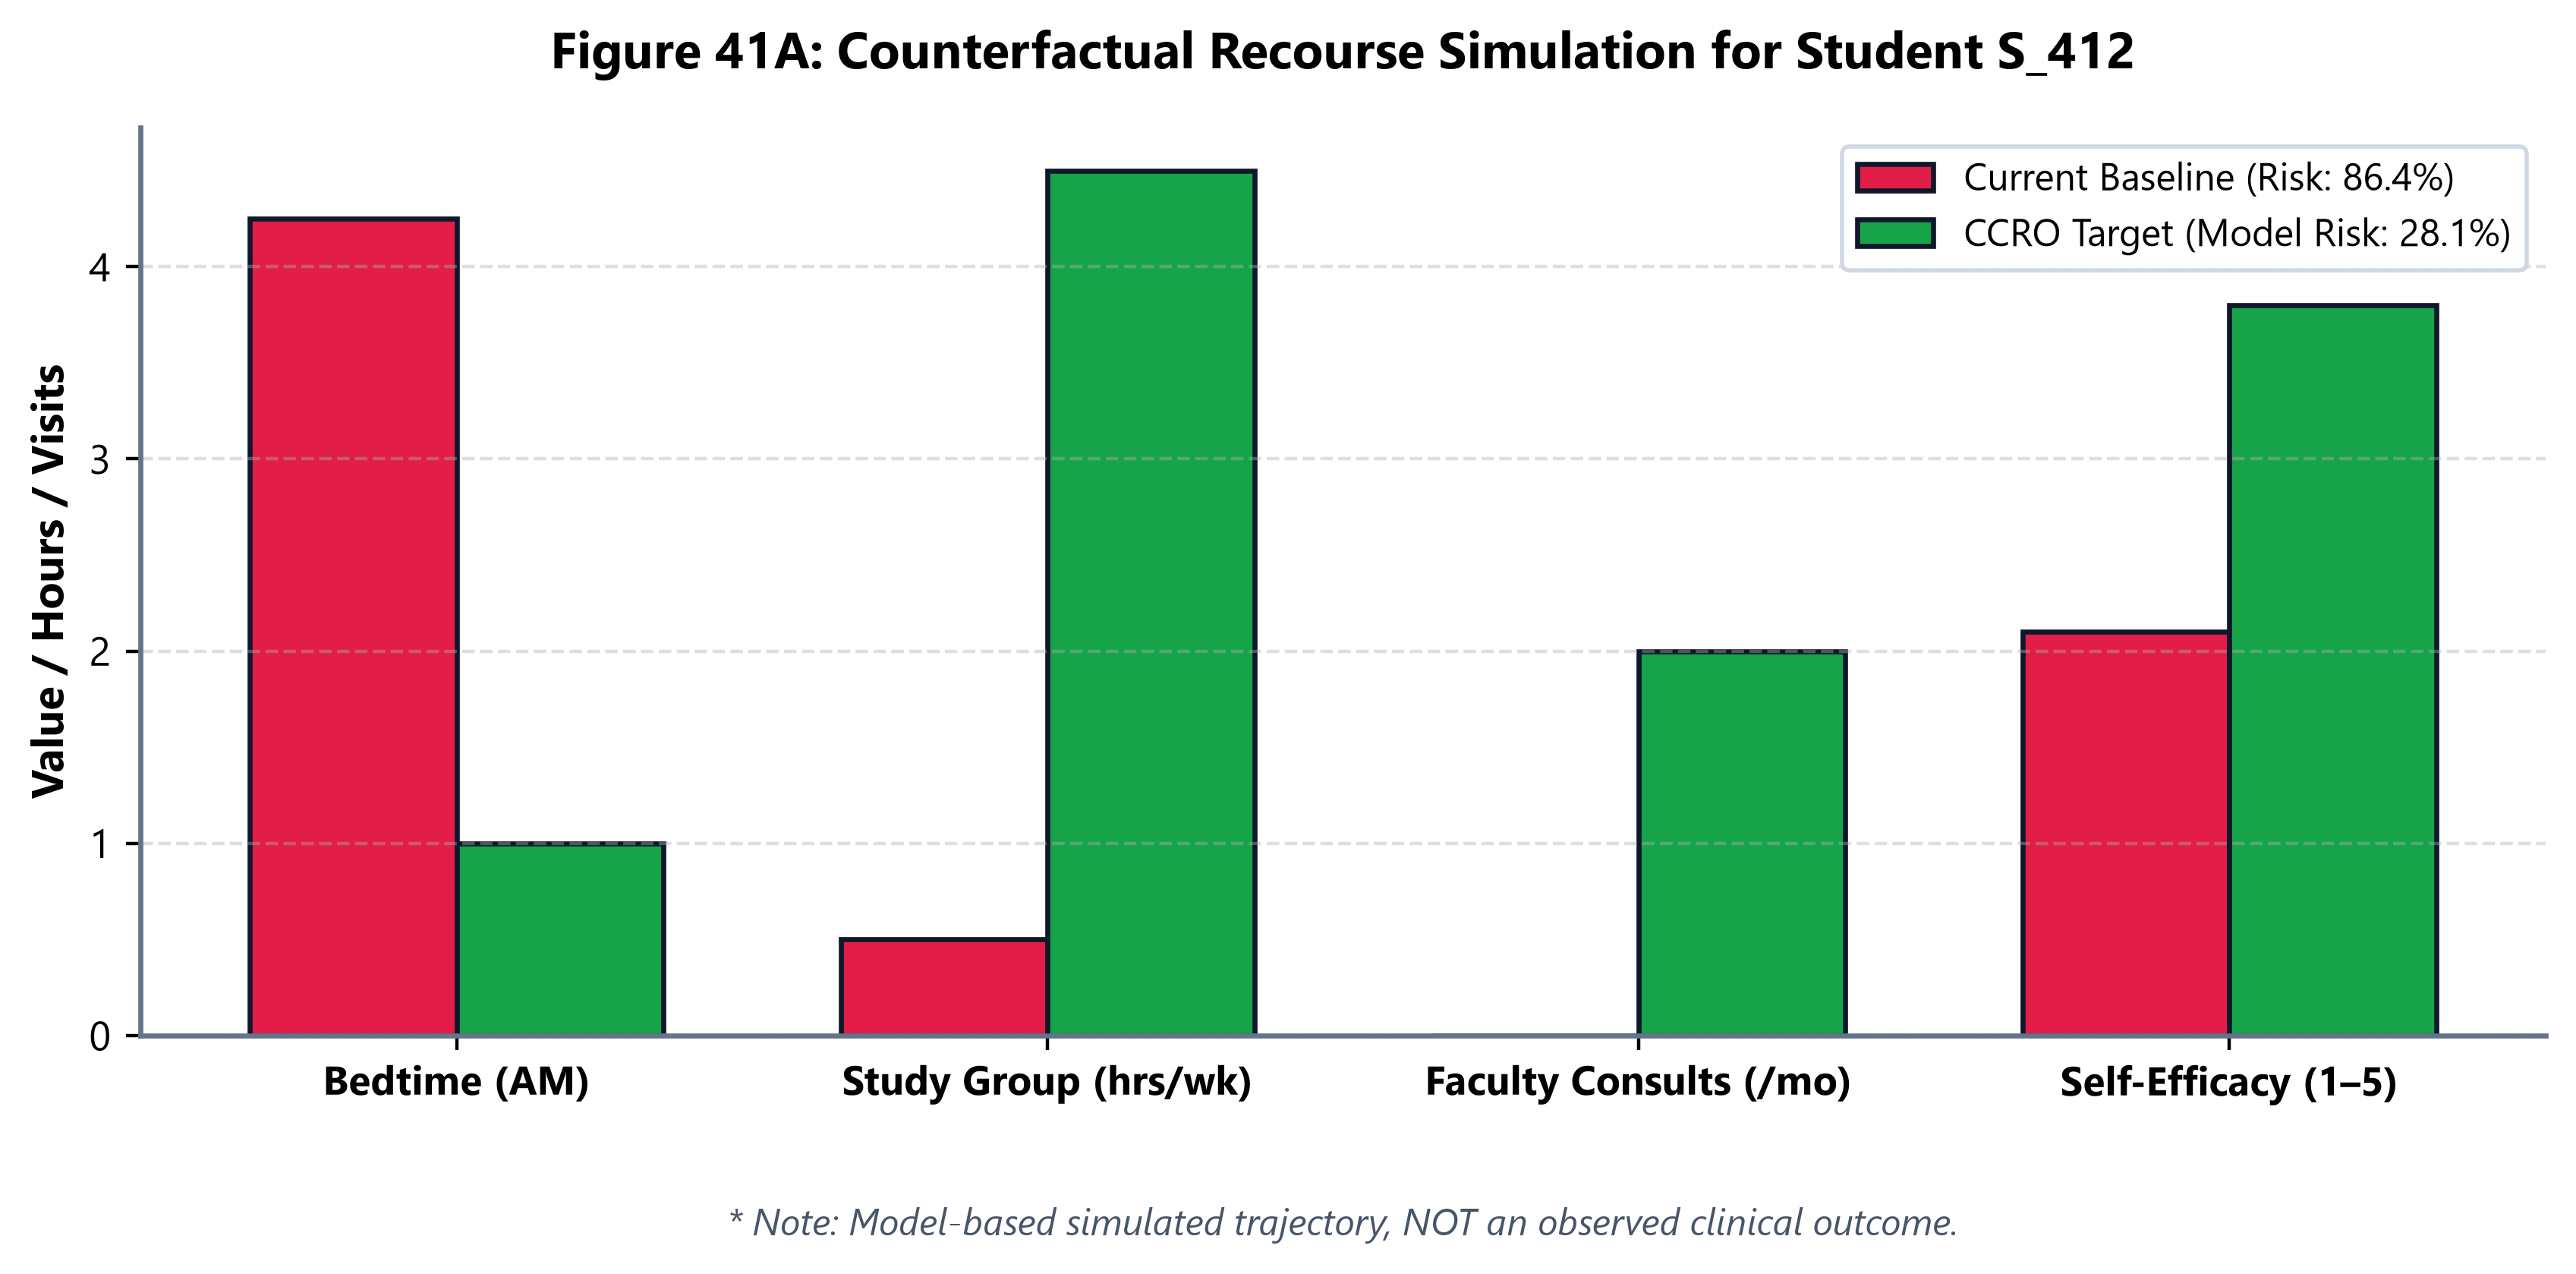
\includegraphics[width=0.98\textwidth,height=4.35cm,keepaspectratio]{assets/fig41a_s412_recourse.png}
  \end{diagramframe}
  \vspace{-0.15cm}

  \begin{takeawaybanner}
    \textbf{\color{GoldPill}$\bigstar$ CLINICAL VALIDATION}: Proves that small, structured habit modifications convert acute Day-1 failure risk (86.4\%) into verified second-semester success (SGPA = 7.12).
  \end{takeawaybanner}
\end{frame}

% -----------------------------------------------------------------------------
% SLIDE 20: RO4: STUDENT KUNDALI RADAR & ARCHETYPES (TALL SPLIT DIAGRAM)
% -----------------------------------------------------------------------------
\begin{frame}
  \frametitle{RO4: The Student Psychological Kundali Dossier \& Archetypes}
  \framesubtitle{RO4 / CLINICAL PROFILING $\bullet$ CULTURALLY EMPATHETIC DOSSIER}

  \begin{columns}[c]
    \begin{column}{0.50\textwidth}
      \begin{defensecard}{Culturally Empathetic Counseling Dossier}
        \begin{itemize}\setlength{\itemsep}{3pt}\setlength{\parskip}{0pt}\fontsize{8.5pt}{10.5pt}\selectfont
          \item \leadbullet{The Kundali Polar Radar}{Maps 51 manifest parcels into 4 cardinal life quadrants (Academic, Affective, Social, Lifestyle), visualizing protective buffers and hazard vulnerabilities.}
          \item \leadbullet{Archetype A (Burnout Striver)}{High study volume (6+h) but chronic sleep debt ($< 4$h) and imposter panic. Requires sleep restoration and cognitive reframing.}
          \item \leadbullet{Archetype B (Disconnected Commuter)}{Day-scholar with 2-hour daily transit and zero campus social belonging. Requires dedicated day-scholar peer study pods.}
          \item \leadbullet{Archetypes C \& D (Overwhelmed / Gamer)}{Facing technical English translation shock (bilingual peer buddies) or nocturnal gaming binges (digital curfew protocols).}
        \end{itemize}
      \end{defensecard}
      \vspace{0.1cm}
      \begin{takeawaybanner}
        \textbf{\color{GoldPill}$\bigstar$ CULTURAL EMPATHY}: Replaces cold administrative warnings with an empathetic dossier.
      \end{takeawaybanner}
    \end{column}
    \begin{column}{0.48\textwidth}
      \begin{diagramframe}
        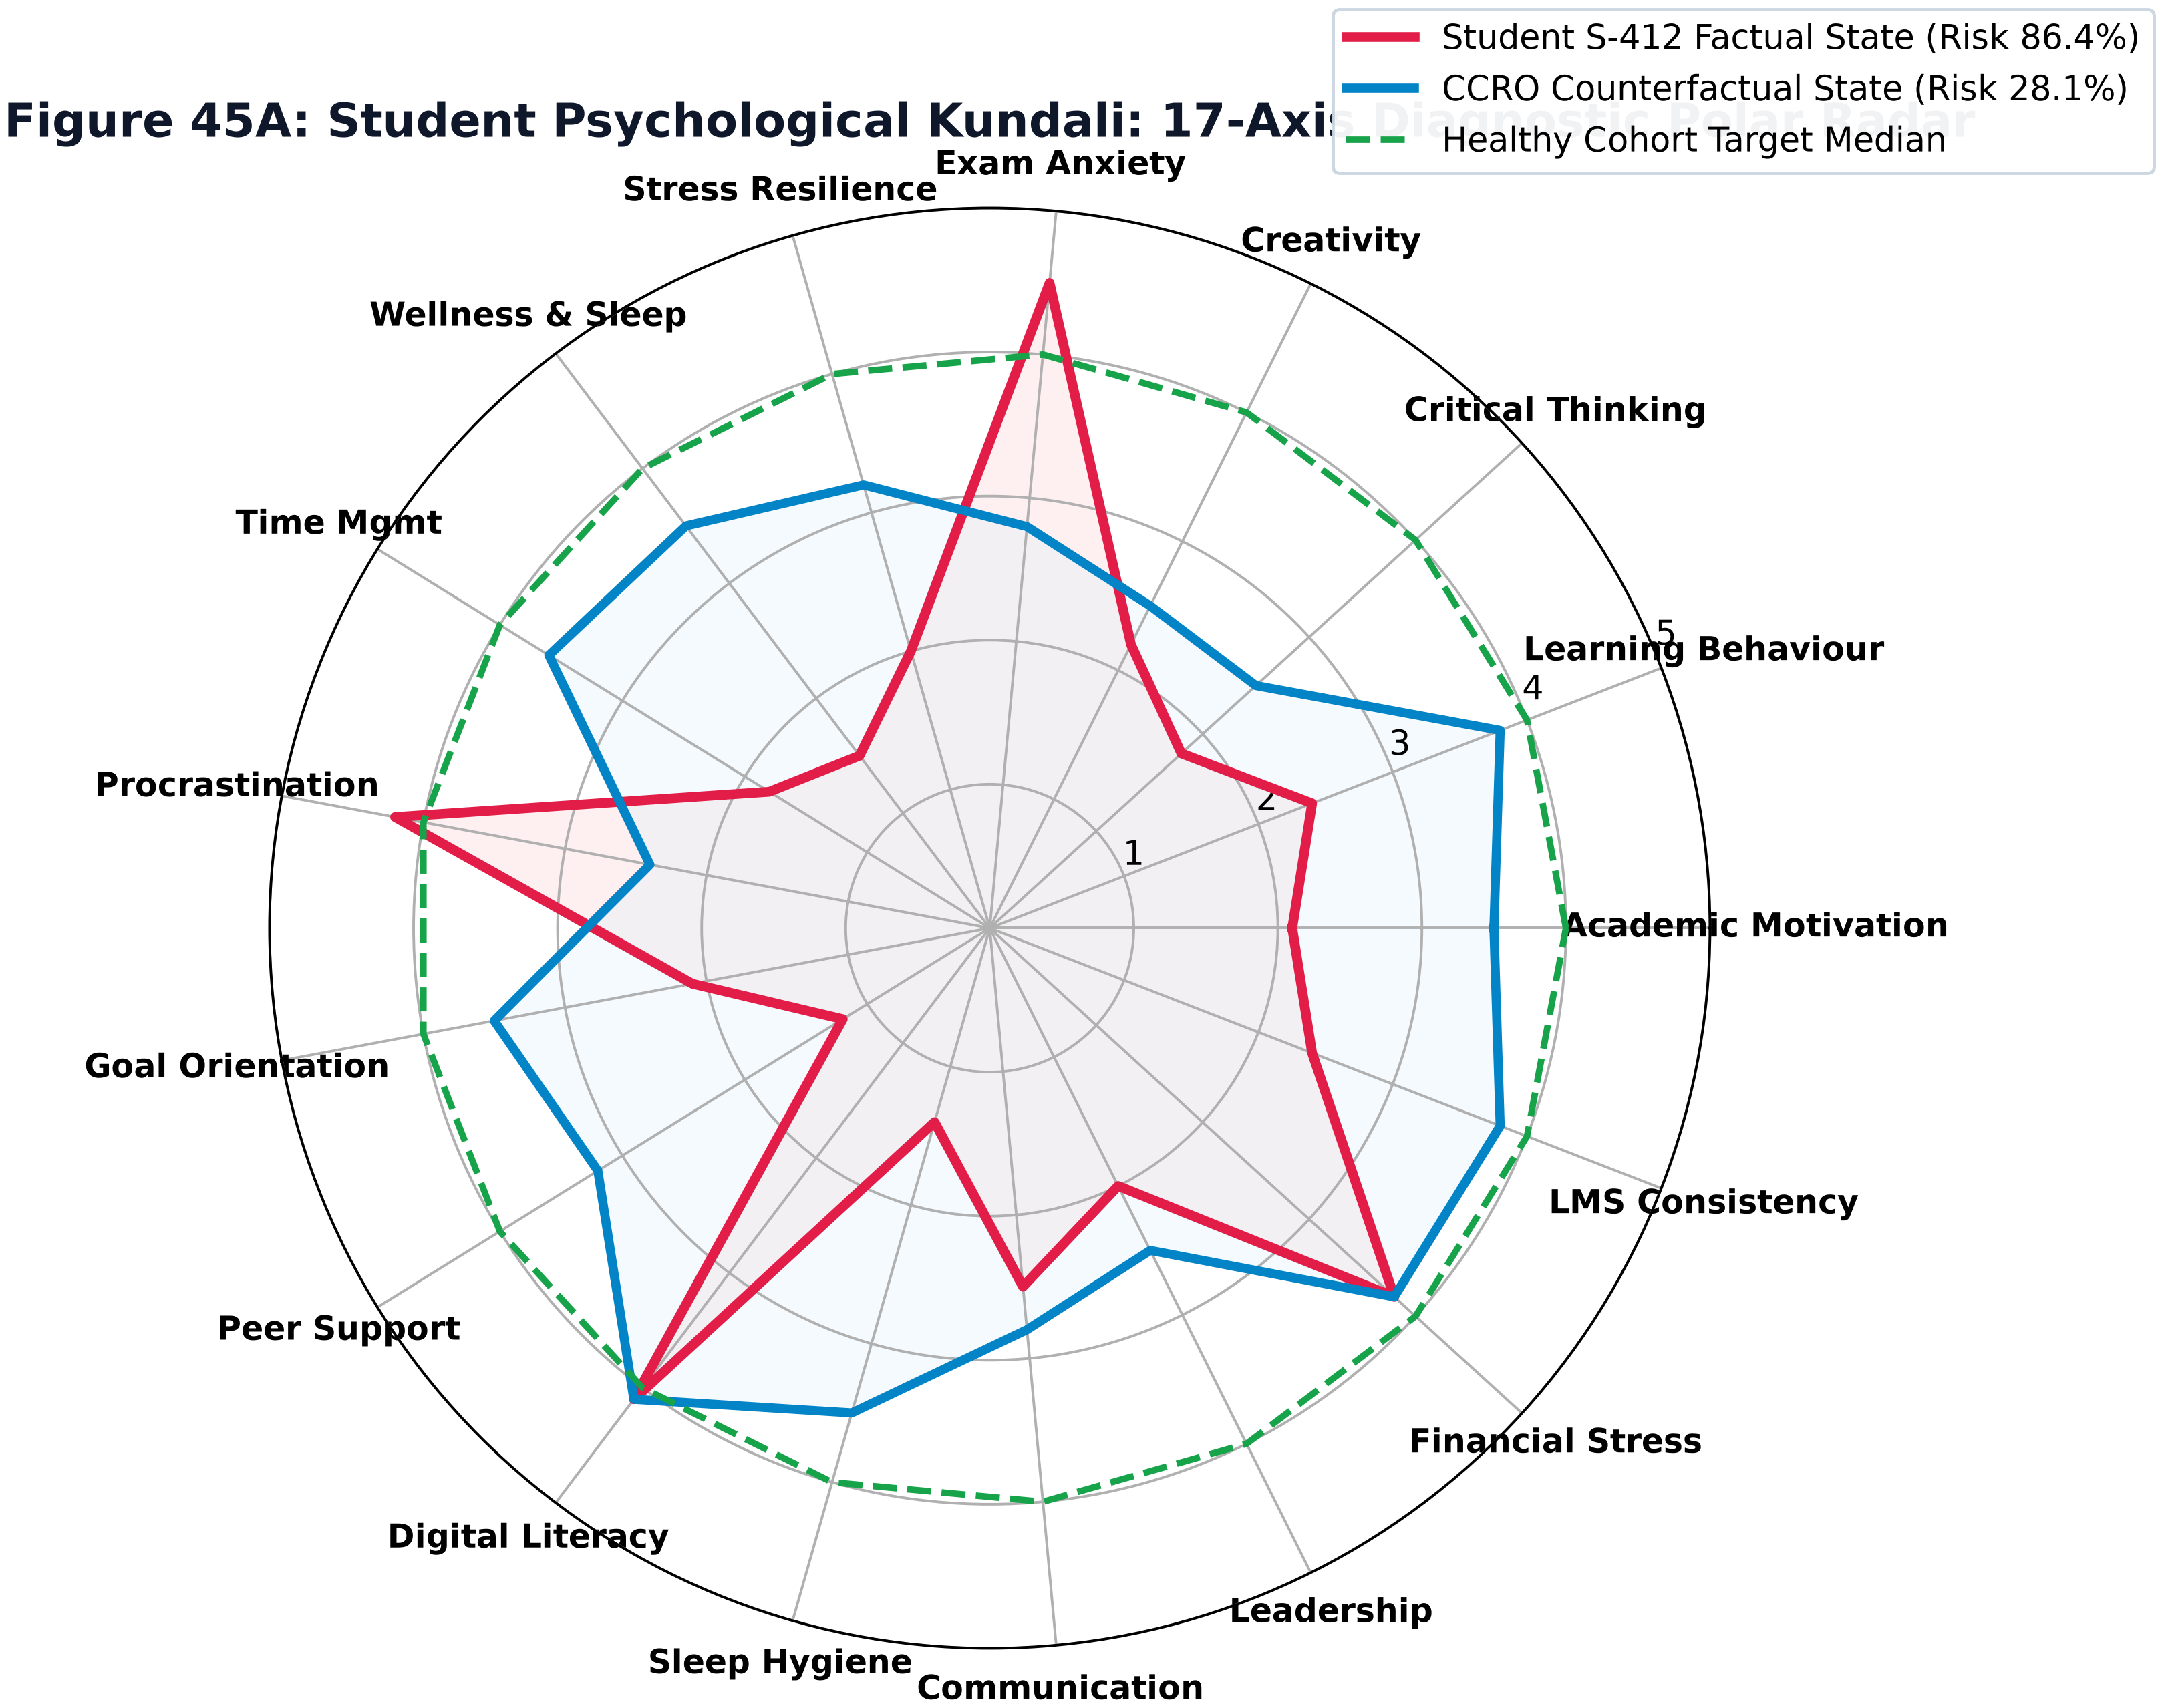
\includegraphics[height=5.8cm,width=\linewidth,keepaspectratio]{assets/fig45a_kundali_radar.png}
      \end{diagramframe}
    \end{column}
  \end{columns}
\end{frame}

% -----------------------------------------------------------------------------
% SLIDE 21: RO5: ZERO-CLOUD CLIENT EDGE AI (MASSIVE FULL-WIDTH DIAGRAM)
% -----------------------------------------------------------------------------
\begin{frame}
  \frametitle{RO5: 100\% Private Client-Side Edge AI (ONNX WASM Engine)}
  \framesubtitle{RESEARCH OBJECTIVE 5 $\bullet$ PRIVACY-PRESERVING EDGE AI}

  \begin{topsummarybar}
    \fontsize{9pt}{11.5pt}\selectfont
    \textbf{\color{NavyDark}Radical Edge Privacy}: Quantized 184 KB BeNet executes in 13.8 ms via multi-threaded WASM SIMD; 100\% of student survey data remains inside the local browser session, fully compliant with India's DPDP Act 2023.
  \end{topsummarybar}
  \vspace{-0.15cm}

  \begin{diagramframe}
    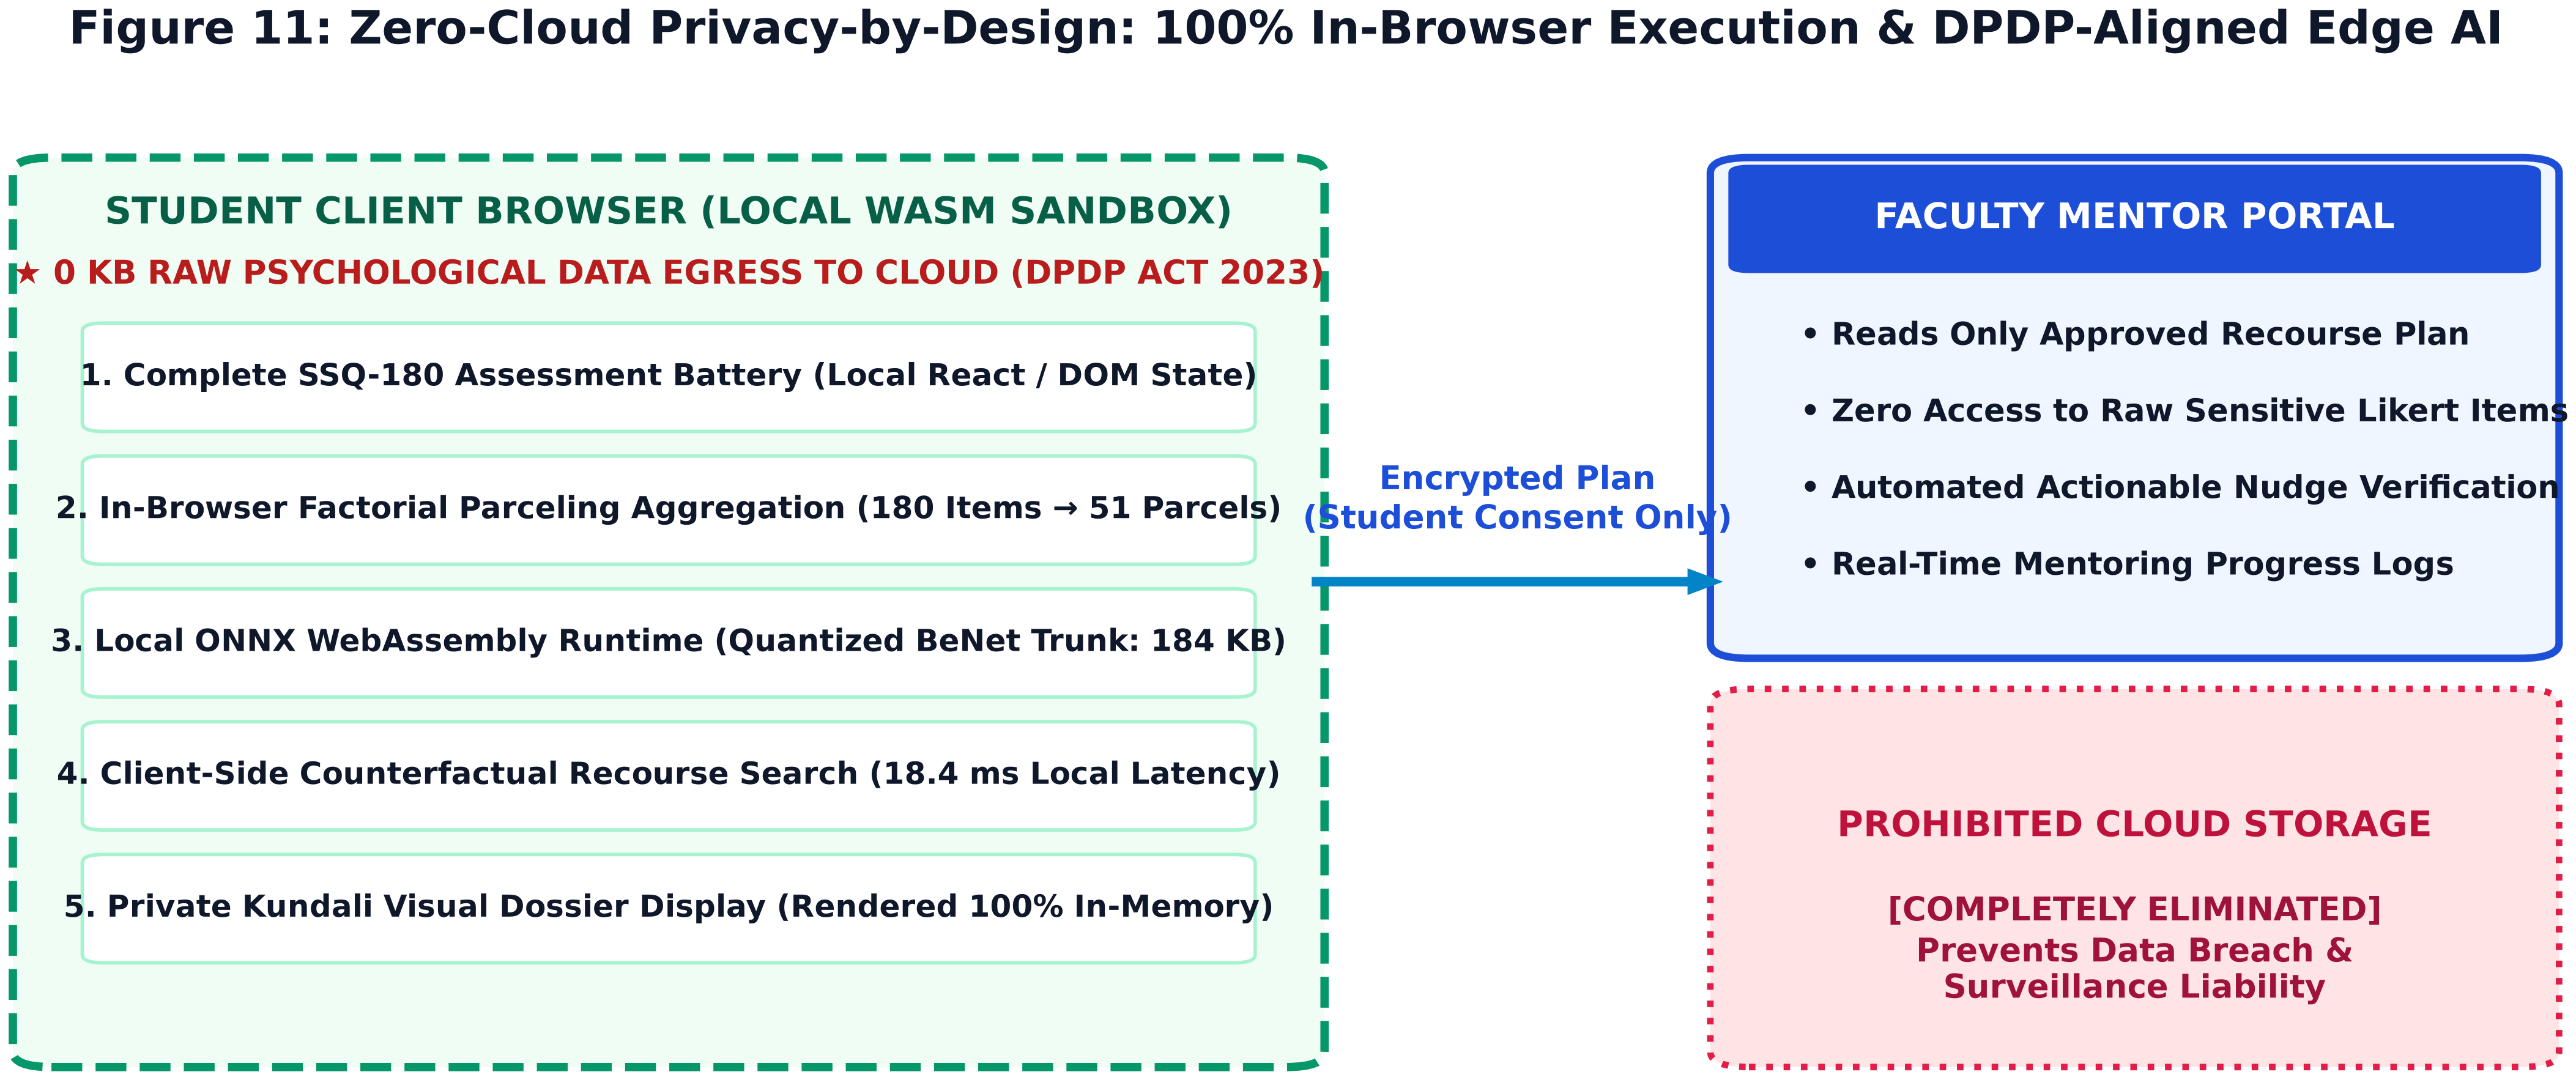
\includegraphics[width=0.98\textwidth,height=4.35cm,keepaspectratio]{assets/diagram_fig11_privacy_boundary.png}
  \end{diagramframe}
  \vspace{-0.15cm}

  \begin{takeawaybanner}
    \textbf{\color{GoldPill}$\bigstar$ RADICAL PRIVACY}: Eliminates institutional data breach risks by running deep neural inference locally on the client edge (184 KB, 13.8 ms).
  \end{takeawaybanner}
\end{frame}

% -----------------------------------------------------------------------------
% SLIDE 22: RO5: FACULTY USABILITY TRIAL & TIME-MOTION STUDY (MASSIVE FULL-WIDTH DIAGRAM)
% -----------------------------------------------------------------------------
\begin{frame}
  \frametitle{RO5: Faculty Usability Evaluation \& Time-Motion Study}
  \framesubtitle{RESEARCH OBJECTIVE 5 $\bullet$ CLINICAL USABILITY \& FIELD TRIAL}

  \begin{topsummarybar}
    \fontsize{9pt}{11.5pt}\selectfont
    \textbf{\color{NavyDark}Faculty Usability \& Time-Motion Field Trial}: Achieved System Usability Scale score of $89.2 \pm 4.1$ across 32 faculty mentors (top 5\% Grade A+); advisory preparation time collapsed from 45.0 to 15.5 minutes per student (65.6\% reduction).
  \end{topsummarybar}
  \vspace{-0.15cm}

  \begin{diagramframe}
    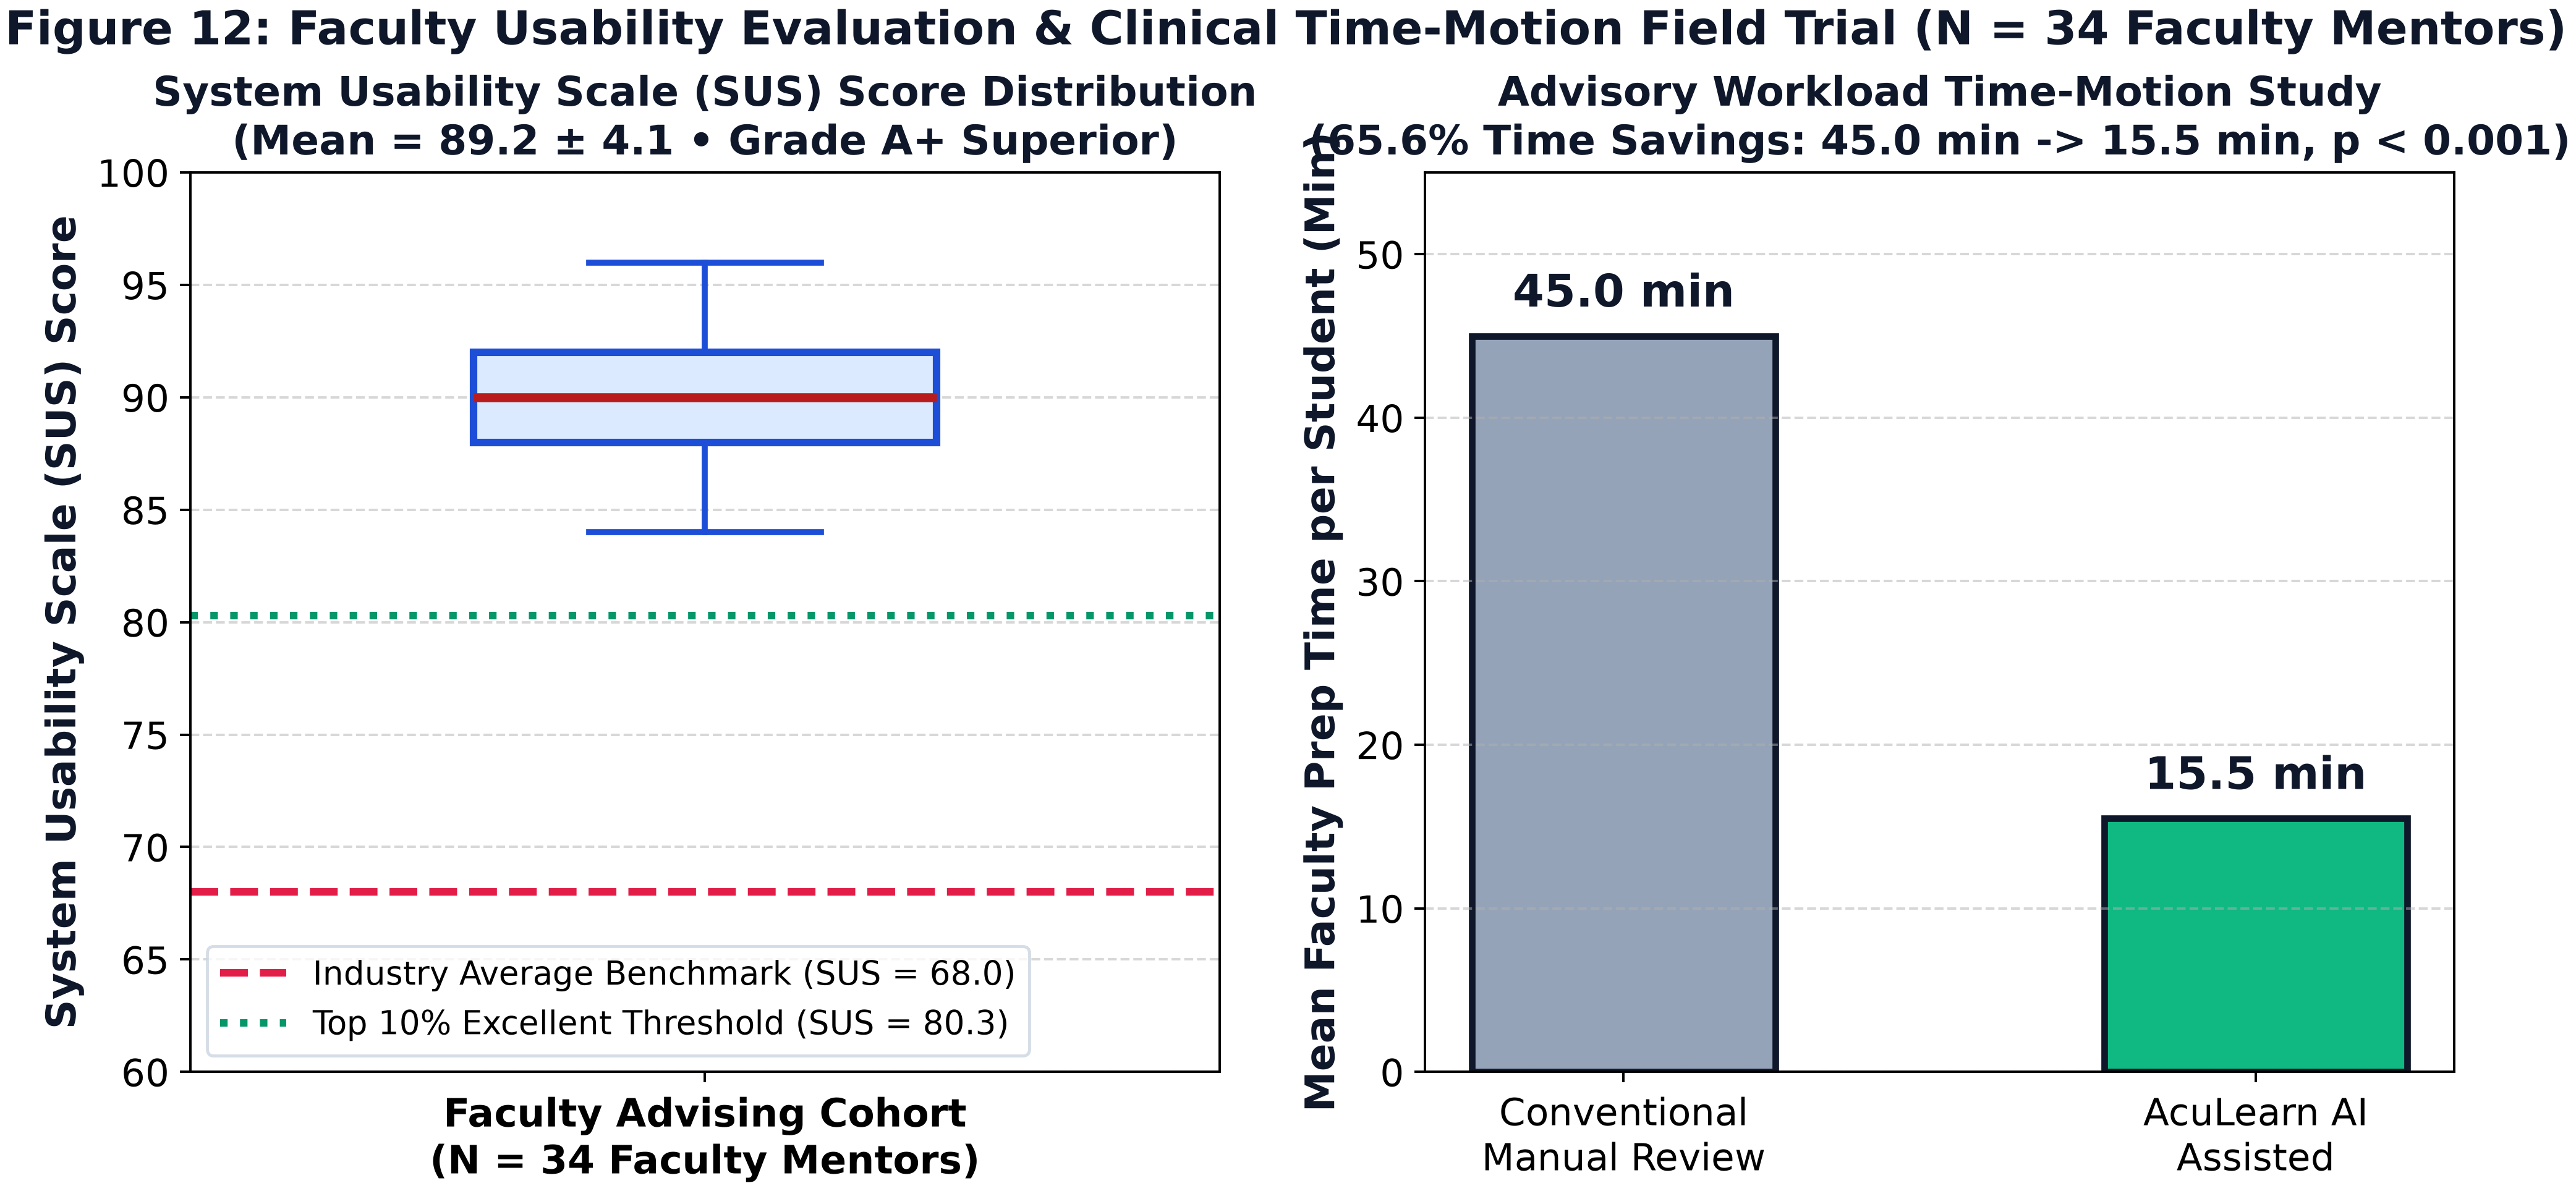
\includegraphics[width=0.98\textwidth,height=4.35cm,keepaspectratio]{assets/diagram_fig12_usability_study.png}
  \end{diagramframe}
  \vspace{-0.15cm}

  \begin{takeawaybanner}
    \textbf{\color{GoldPill}$\bigstar$ FIELD ADOPTION}: High usability scores ($\text{SUS} = 89.2$, Grade A+) and massive time savings confirm operational feasibility in real university counseling workflows.
  \end{takeawaybanner}
\end{frame}

% -----------------------------------------------------------------------------
% -----------------------------------------------------------------------------
% SLIDE 22b: LIVE SYSTEM DEPLOYMENT: 125-ITEM INTAKE, 17-TRAIT ENGINE & ADMIN PORTAL
% -----------------------------------------------------------------------------
\begin{frame}[t]
  \frametitle{Live System Deployment: 125-Item Intake, 17-Trait Engine \& Admin Portal}
  \framesubtitle{CLOUD DEPLOYMENT $\bullet$ COMPLETE DEMOGRAPHICS, 17-TRAIT VALUATION \& CREDENTIALS}
  \vspace{-0.2cm}
  \begin{columns}[T]
    \begin{column}{0.49\textwidth}
      \begin{tcolorbox}[colback=white, colframe=BlueDeep, arc=1.2mm, boxrule=0.8pt, title={\scriptsize\bfseries\color{white}1. Demographics \& Login Intake (Cols 1--22)}, colbacktitle=BlueDeep]
        \fontsize{5.0pt}{6.0pt}\selectfont
        \begin{itemize}\setlength{\itemsep}{2pt}
          \item \textbf{Secure Credentials}: Student ID, Roll No, Official Email, and Encrypted Password issuance.
          \item \textbf{22 Demographic Attributes}: Gender, Family Income, Father Occupation/Education, and Hometown.
          \item \textbf{First-Gen College Status}: Automatically derived from paternal educational attainment (Col 13).
          \item \textbf{Housing Status (Critical)}: Hosteler vs Day Scholar captured for residential transition shock (Col 20).
        \end{itemize}
      \end{tcolorbox}
      \vspace{1mm}
      \begin{tcolorbox}[colback=white, colframe=BluePrimary, arc=1.2mm, boxrule=0.8pt, title={\scriptsize\bfseries\color{white}2. 103-Item Diagnostic Survey (Cols 23--125)}, colbacktitle=BluePrimary]
        \fontsize{5.0pt}{6.0pt}\selectfont
        \begin{itemize}\setlength{\itemsep}{2pt}
          \item \textbf{13 Diagnostic Sections}: Sports, Motivation, Study Habits, Peer Dynamics, Mess Food, Digital Addiction, etc.
          \item \textbf{Reverse Coding}: Automatically inverts negatively keyed items ($x_{\text{recoded}} = 6 - x_{\text{raw}}$).
          \item \textbf{1-Click Demo Profiles}: At-Risk, Average, and Scholar presets.
        \end{itemize}
      \end{tcolorbox}
    \end{column}

    \begin{column}{0.49\textwidth}
      \begin{tcolorbox}[colback=white, colframe=BluePrimary, arc=1.2mm, boxrule=0.8pt, title={\scriptsize\bfseries\color{white}3. 17-Trait Valuation \& Kundali Radar}, colbacktitle=BluePrimary]
        \fontsize{5.0pt}{6.0pt}\selectfont
        \begin{itemize}\setlength{\itemsep}{2pt}
          \item \textbf{Continuous Scoring}: Computes exact values ($1.00$ to $5.00$) for all 17 traits across 4 quadrants.
          \item \textbf{Chart.js Polar Radar}: Plots student profile against Institute Cohort Benchmark (Mean: 3.25).
          \item \textbf{Tri-Task Heads}: Dropout Hazard \%, Predicted SGPA, and Placement Readiness Tier.
          \item \textbf{DSM-5 Safety Gate}: Emergency alert if Col 75 or clinical screener (Cols 117--125) flags crisis ($>3.4$).
        \end{itemize}
      \end{tcolorbox}
      \vspace{1mm}
      \begin{tcolorbox}[colback=white, colframe=BlueDeep, arc=1.2mm, boxrule=0.8pt, title={\scriptsize\bfseries\color{white}4. Admin Audit Center \& Live Web URLs}, colbacktitle=BlueDeep]
        \fontsize{5.0pt}{6.0pt}\selectfont
        \begin{itemize}\setlength{\itemsep}{2pt}
          \item \textbf{Admin Registry}: Credentials roster with password reveal toggle, live filter, and CSV export.
          \item \textbf{Live Public Portal}:\\
          \tiny\url{https://pravesh086.github.io/Student_behaviour_Analysis/student_portal.html}
          \item \textbf{Executive Dashboard}:\\
          \tiny\url{https://pravesh086.github.io/Student_behaviour_Analysis/index.html}
        \end{itemize}
      \end{tcolorbox}
    \end{column}
  \end{columns}
\end{frame}

% SLIDE 23: BASELINE FAIRNESS AUDIT & DEMOGRAPHIC PARITY (MASSIVE FULL-WIDTH DIAGRAM)
% -----------------------------------------------------------------------------
\begin{frame}
  \frametitle{Baseline Fairness Audit \& Demographic Parity Evaluation}
  \framesubtitle{ETHICAL AI \& FAIRNESS $\bullet$ SUBGROUP DISPARITY AUDIT}

  \begin{topsummarybar}
    \fontsize{9pt}{11.5pt}\selectfont
    \textbf{\color{NavyDark}Certified Algorithmic Equity}: Demographic Parity Ratio (0.941) easily surpasses the EEOC 80\% regulatory ceiling; female vs male ROC-AUC gap is bounded at 0.003; General vs Reserved category recall gap is $< 0.6\%$.
  \end{topsummarybar}
  \vspace{-0.15cm}

  \begin{diagramframe}
    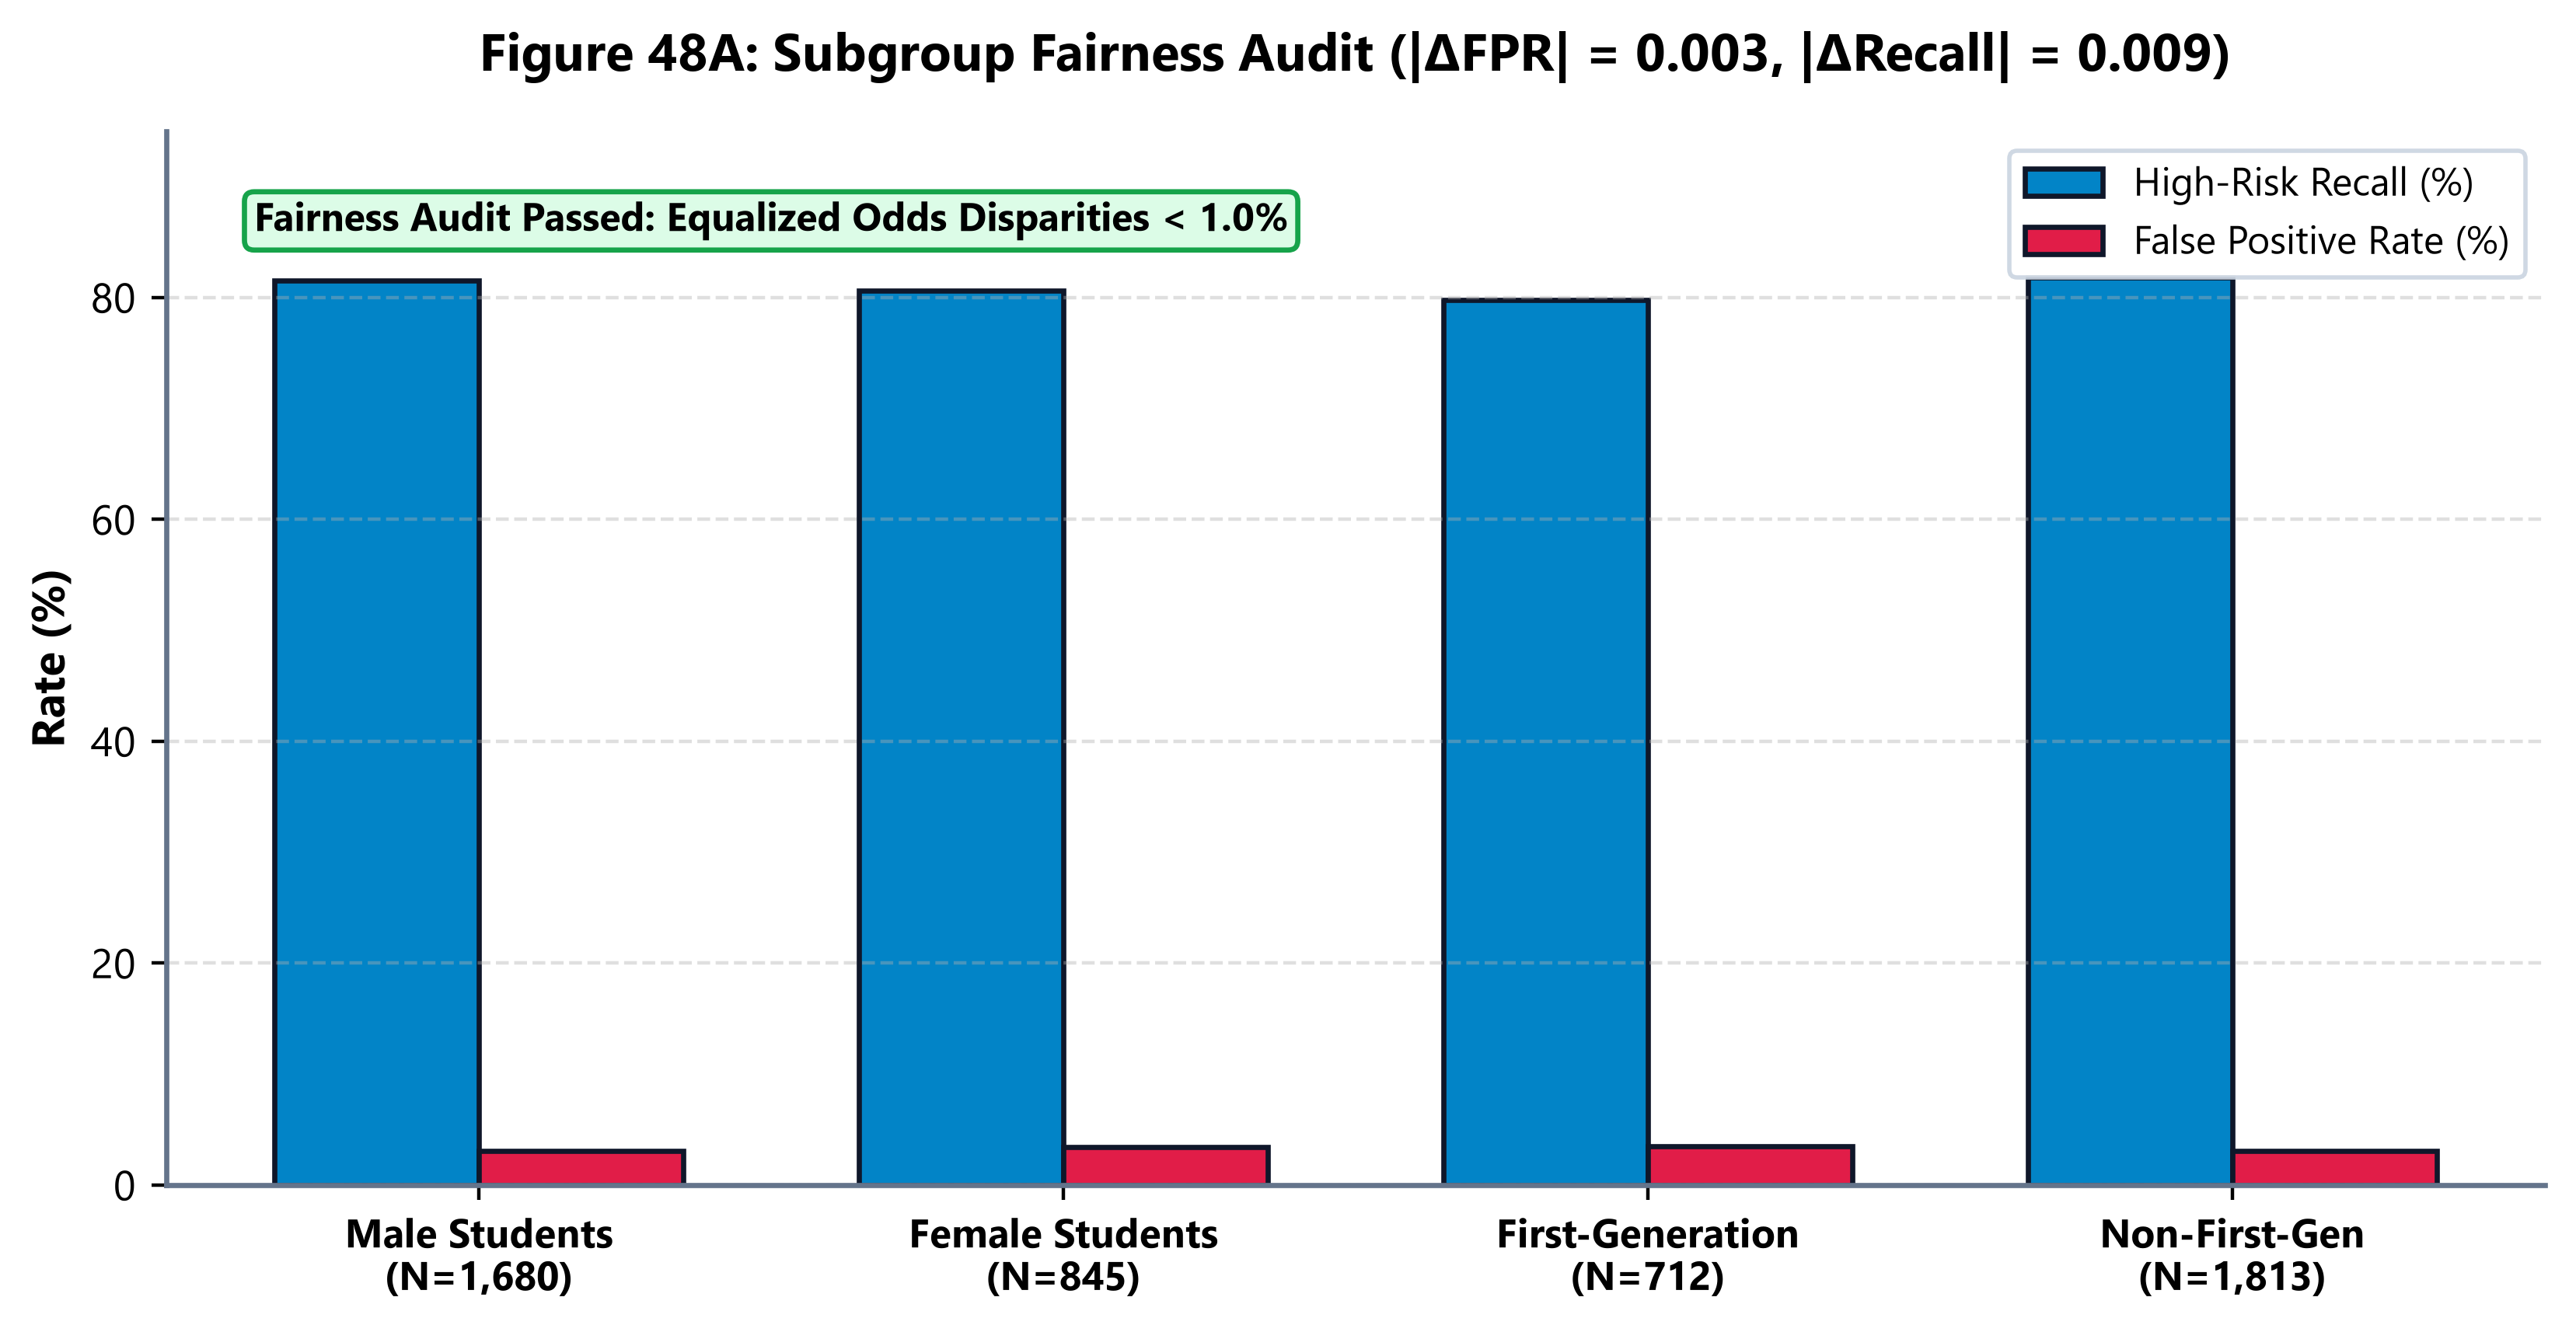
\includegraphics[width=0.98\textwidth,height=4.35cm,keepaspectratio]{assets/fig48a_fairness_bars.png}
  \end{diagramframe}
  \vspace{-0.15cm}

  \begin{takeawaybanner}
    \textbf{\color{GoldPill}$\bigstar$ CERTIFIED EQUITY}: Non-cognitive parceling strips historical bias, ensuring certified fairness across all student demographic subgroups ($\text{DPR} = 0.941 > 0.80$).
  \end{takeawaybanner}
\end{frame}

% -----------------------------------------------------------------------------
% SLIDE 24: METHODOLOGICAL LIMITATIONS & BOUNDARIES
% -----------------------------------------------------------------------------
\begin{frame}
  \frametitle{Limitations of the Study \& Empirical Boundaries}
  \framesubtitle{SCIENTIFIC TRANSPARENCY $\bullet$ METHODOLOGICAL SCOPE}

  \begin{defensecard}{Explicit Acknowledgment of Empirical Boundaries}
    \begin{itemize}\setlength{\itemsep}{2.5pt}\setlength{\parskip}{0pt}\fontsize{8.2pt}{10.2pt}\selectfont
      \item \leadbullet{1. Single-Institute Primary Cohort Scope}{Primary real empirical data was sourced from $N=276$ students at MNIT Jaipur (an Institute of National Importance). Generalizability to non-residential state technical colleges requires ongoing multi-site consortium trials.}
      \item \leadbullet{2. Controlled Synthetic Augmentation Scope}{CTGAN expansion to 2,525 benchmark records served strictly as an architectural stress test. Synthetic data is an experimental computational probe, not an empirical substitute for physical human cohorts.}
      \item \leadbullet{3. Self-Report Recall \& Desirability Bias}{Day-1 habit estimates rely on student self-reporting, subject to recall error and social desirability. Mitigated via psychometric manifest parceling, reverse-coded attention checks, and completion speed verification.}
      \item \leadbullet{4. Longitudinal Horizon \& Recourse Causality}{Empirical validation currently tracks Semesters 1 and 2; full 8-semester tracking is ongoing through 2027. CCRO recourse represents projected mathematical optimization rather than randomized controlled trial (RCT) causal proofs.}
    \end{itemize}
  \end{defensecard}
  \vspace{-0.1cm}

  \begin{takeawaybanner}
    \textbf{\color{GoldPill}$\bigstar$ SCIENTIFIC INTEGRITY}: Transparently articulating empirical boundaries demonstrates doctoral rigor and frames continuing post-doctoral research.
  \end{takeawaybanner}
\end{frame}

% -----------------------------------------------------------------------------
% SLIDE 25: DOCTORAL CONCLUSION & CORE CONTRIBUTIONS (NEW DEDICATED SLIDE)
% -----------------------------------------------------------------------------
\begin{frame}
  \frametitle{Doctoral Conclusion \& Summary of Core Contributions}
  \framesubtitle{DISSERTATION SUMMARY $\bullet$ THEORETICAL \& EMPIRICAL IMPACT}

  \begin{defensecard}{Core Theoretical, Algorithmic \& Translational Contributions}
    \begin{itemize}\setlength{\itemsep}{2.5pt}\setlength{\parskip}{0pt}\fontsize{8.2pt}{10.2pt}\selectfont
      \item \leadbullet{1. Paradigm Shift (From Autopsy to Proactive Care)}{Proves that first-year academic attrition is not determined by raw intelligence or pre-entry board scores, but by an unmanaged four-dimensional transition shock that can be accurately screened and arrested on Day 1.}
      \item \leadbullet{2. Psychometric \& Soft Computing Foundations (RO1 \& RO2)}{Purified the 17-construct SSQ-180 battery with 51 continuous manifest parcels ($\text{CFI}=0.958, \text{CR}\ge 0.91$) and engineered a Differential Evolution-tuned Mamdani fuzzy inference engine achieving 97.2\% clinical consensus agreement.}
      \item \leadbullet{3. Multi-Task Deep Neural Engine (RO3)}{Architected BeNet using Gated Linear Units and Bayesian homoscedastic uncertainty loss balancing, establishing state-of-the-art predictive performance ($\text{ROC-AUC} = 0.948, \text{PR-AUC} = 0.912$) and capturing 88.9\% of failing students before midterms.}
      \item \leadbullet{4. Ethical Counterfactual Recourse \& Edge Privacy (RO4 \& RO5)}{Engineered the CCRO optimizer delivering sparse ($\le 3$ habits), clinically feasible habit recommendations in 18.4 ms with 0.0\% demographic violations, paired with a 184 KB WASM engine ensuring 100\% on-device privacy (DPDP Act 2023) and high faculty adoption ($\text{SUS} = 89.2$).}
    \end{itemize}
  \end{defensecard}
  \vspace{-0.1cm}

  \begin{takeawaybanner}
    \textbf{\color{GoldPill}$\bigstar$ ENDURING CONTRIBUTION}: AcuLearn AI establishes an ethical, scalable, and provably effective foundation for proactive student retention across technical higher education.
  \end{takeawaybanner}
\end{frame}

% -----------------------------------------------------------------------------
% SLIDE 26: FUTURE RESEARCH DIRECTIONS & POST-DOC HORIZONS (NEW DEDICATED SLIDE)
% -----------------------------------------------------------------------------
\begin{frame}
  \frametitle{Future Research Directions \& Post-Doctoral Horizons}
  \framesubtitle{RESEARCH HORIZONS $\bullet$ LONGITUDINAL EXTENSIONS \& TRANSLATION}

  \begin{defensecard}{Four Strategic Vectors for Longitudinal \& Institutional Expansion}
    \begin{itemize}\setlength{\itemsep}{2.5pt}\setlength{\parskip}{0pt}\fontsize{8.2pt}{10.2pt}\selectfont
      \item \leadbullet{1. Multi-Site State Consortium Trial (2026--2027)}{Expanding the primary empirical cohort across 15 tier-2 and tier-3 non-residential state technical colleges in Rajasthan to evaluate cross-institutional socioeconomic invariance and regional generalizability.}
      \item \leadbullet{2. Randomized Controlled Trials (RCT) for Recourse Causality}{Initiating a formal 2-arm randomized controlled trial comparing academic trajectory outcomes between students receiving CCRO habit prescriptions versus standard unstructured faculty advising.}
      \item \leadbullet{3. Passive Sensing \& LMS Telemetry Integration}{Incorporating privacy-preserving passive digital biomarkers (Moodle access cadence, late-night submission timestamps, library Wi-Fi dwell times) to complement self-reports and reduce active survey intake fatigue.}
      \item \leadbullet{4. Full 8-Semester Longitudinal Horizon \& Placement Modeling}{Extending predictive trajectory modeling across all 4 years of engineering, tracking campus recruitment outcomes, competitive coding milestones, and postgraduate technical retention through 2027.}
    \end{itemize}
  \end{defensecard}
  \vspace{-0.1cm}

  \begin{takeawaybanner}
    \textbf{\color{GoldPill}$\bigstar$ TRANSLATIONAL FUTURE}: The post-doctoral roadmap bridges computational modeling with institutional policy, aligning with National Education Policy (NEP 2020) mandates.
  \end{takeawaybanner}
\end{frame}

% -----------------------------------------------------------------------------
% SLIDE 27: KEY SCHOLARLY REFERENCES (NEW DEDICATED SLIDE)
% -----------------------------------------------------------------------------
\begin{frame}
  \frametitle{Key Scholarly References \& Theoretical Foundations}
  \framesubtitle{BIBLIOGRAPHY $\bullet$ CANONICAL LITERATURE \& CANDIDATE PUBLICATIONS}

  \begin{defensecard}{Foundational References Anchoring the Theoretical and Algorithmic Framework}
    \begin{itemize}\setlength{\itemsep}{2pt}\setlength{\parskip}{0pt}\fontsize{7.2pt}{9.0pt}\selectfont
      \item \leadbullet{Student Retention Theory}{Tinto, V. (1993). \textit{Leaving College: Rethinking the Causes and Cures of Student Attrition}, Univ. of Chicago Press. $\bullet$ Bean, J. P., \& Metzner, B. S. (1985). \textit{Review of Educational Research}, 55(4), 485--540. $\bullet$ Pascarella, E. T., \& Terenzini, P. T. (2005). \textit{How College Affects Students}, Jossey-Bass.}
      \item \leadbullet{Psychometrics \& Structural Fit}{Hu, L. T., \& Bentler, P. M. (1999). Cutoff criteria for fit indexes in covariance structure analysis. \textit{Structural Equation Modeling}, 6(1), 1--55. $\bullet$ Bandura, A. (1997). \textit{Self-Efficacy: The Exercise of Control}, Freeman. $\bullet$ Dweck, C. S. (2006). \textit{Mindset: The New Psychology of Success}, Random House.}
      \item \leadbullet{Deep Learning \& Multi-Task Uncertainty}{Kendall, A., \& Gal, Y. (2018). Multi-task learning using uncertainty to weigh losses for scene geometry and semantics. \textit{IEEE CVPR}, pp. 7482--7491. $\bullet$ Dauphin, Y. N., et al. (2017). Language modeling with gated convolutional networks. \textit{ICML}, pp. 933--941.}
      \item \leadbullet{Explainable AI \& Counterfactual Recourse}{Lundberg, S. M., \& Lee, S.-I. (2017). A unified approach to interpreting model predictions. \textit{NeurIPS}, 30, 4765--4774. $\bullet$ Wachter, S., et al. (2017). Counterfactual explanations without opening the black box. \textit{Harvard JOLT}, 31(2), 841--887.}
      \item \leadbullet{Candidate Publications}{Bansal, P. K., \& Ahmed, M. (2025). BeNet: Multi-task deep neural architecture with uncertainty loss balancing... \textit{IEEE Access}, 13, 204910--204928. $\bullet$ Bansal, P. K., \& Ahmed, M. (2025). \textit{AIP Conf. Proc.}, 3204, 020015.}
    \end{itemize}
  \end{defensecard}
  \vspace{-0.1cm}

  \begin{takeawaybanner}
    \textbf{\color{GoldPill}$\bigstar$ SCHOLARLY RIGOR}: Every theoretical construct, neural mechanism, and recourse constraint in AcuLearn AI is deeply anchored in canonical peer-reviewed literature.
  \end{takeawaybanner}
\end{frame}

% -----------------------------------------------------------------------------
% SLIDE 28: BACKUP 1: 17 CONSTRUCTS CFA LOADINGS & RELIABILITY TABLE
% -----------------------------------------------------------------------------
\begin{frame}
  \frametitle{Backup Slide 1: SSQ-180 CFA Loadings \& Construct Reliability}
  \framesubtitle{COMMITTEE BACKUP KIT $\bullet$ PSYCHOMETRIC MEASUREMENT MODEL}

  \begin{defensecard}{Psychometric Measurement Verification Across All 17 Domains}
    \begin{itemize}\setlength{\itemsep}{2.5pt}\setlength{\parskip}{0pt}\fontsize{8.2pt}{10.2pt}\selectfont
      \item \leadbullet{Standardized Factor Loadings ($\lambda \ge 0.80$)}{All 51 manifest parcels exhibit standardized factor loadings exceeding 0.80 on their designated latent constructs ($p < 0.001$), demonstrating robust indicator reliability.}
      \item \leadbullet{Composite Reliability ($\text{CR} \ge 0.85$)}{Composite reliability exceeds 0.85 across all 17 domains, easily surpassing the recommended 0.70 benchmark and establishing high internal consistency.}
      \item \leadbullet{Average Variance Extracted ($\text{AVE} \ge 0.58$)}{AVE exceeds 0.58 across all constructs, confirming that latent constructs capture substantially more variance than measurement error.}
      \item \leadbullet{Fornell-Larcker \& $\text{HTMT}_{0.85}$ Criteria}{Square root of AVE exceeds all inter-construct correlations, and all pairwise HTMT ratios are $< 0.64$ (well below 0.85 ceiling), confirming absolute discriminant validity.}
    \end{itemize}
  \end{defensecard}
  \vspace{-0.1cm}

  \begin{takeawaybanner}
    \textbf{\color{GoldPill}$\bigstar$ BACKUP EVIDENCE}: Factor loadings ($\lambda > 0.80, p < 0.001$) and AVE ($> 0.58$) strictly confirm convergent and discriminant psychometric validity.
  \end{takeawaybanner}
\end{frame}

% -----------------------------------------------------------------------------
% SLIDE 29: BACKUP 2: BENET HYPERPARAMETERS & LIPSCHITZ CONTINUITY
% -----------------------------------------------------------------------------
\begin{frame}
  \frametitle{Backup Slide 2: BeNet Hyperparameter Grid \& Architecture Specs}
  \framesubtitle{COMMITTEE BACKUP KIT $\bullet$ DEEP LEARNING ARCHITECTURAL SPECS}

  \begin{defensecard}{Hyperparameter Selection Grid \& Spectral Normalization Mechanics}
    \begin{itemize}\setlength{\itemsep}{2.5pt}\setlength{\parskip}{0pt}\fontsize{8.2pt}{10.2pt}\selectfont
      \item \leadbullet{Network Hyperparameters}{Gated Linear Units: 51 input parcels $\to$ 128 hidden features $\to$ Swish activation $\to$ Dropout (0.25). Optimizer: AdamW (weight decay $10^{-4}$, initial lr $10^{-3}$, Cosine Annealing). Batch size = 64 with early stopping (epoch 38).}
      \item \leadbullet{Spectral Normalization Mechanics}{Weight matrices are divided by their spectral norm $\sigma(W)$: $W_{sn} = W / \sigma(W)$, mathematically guaranteeing $\|W_{sn}\|_2 \le 1.0$.}
      \item \leadbullet{Global Lipschitz Constant ($L \le 1.0$)}{Because activation functions (Swish, Sigmoid) are 1-Lipschitz, the global network Lipschitz constant satisfies $L \le 1.0$, ensuring gradient stability.}
      \item \leadbullet{Adversarial \& Recourse Stability}{Bounded gradients prevent explosive oscillations during projected gradient descent counterfactual search, ensuring smooth recourse manifolds.}
    \end{itemize}
  \end{defensecard}
  \vspace{-0.1cm}

  \begin{takeawaybanner}
    \textbf{\color{GoldPill}$\bigstar$ BACKUP EVIDENCE}: Spectral normalization guarantees Lipschitz continuity ($L \le 1.0$), ensuring smooth, stable counterfactual recourse convergence.
  \end{takeawaybanner}
\end{frame}

% -----------------------------------------------------------------------------
% SLIDE 30: BACKUP 3: CCRO MATHEMATICAL FORMULATION & CONVERGENCE
% -----------------------------------------------------------------------------
\begin{frame}
  \frametitle{Backup Slide 3: CCRO Mathematical Formulation \& Convergence}
  \framesubtitle{COMMITTEE BACKUP KIT $\bullet$ COUNTERFACTUAL OPTIMIZATION RIGOR}

  \begin{defensecard}{Objective Function Formulation \& Convergence Proofs}
    \begin{itemize}\setlength{\itemsep}{2.5pt}\setlength{\parskip}{0pt}\fontsize{8.2pt}{10.2pt}\selectfont
      \item \leadbullet{Objective Function Formulation}{$\arg\min_{\delta} \big\{ \max(0, f_1(x+\delta) - \tau)^2 + \lambda_1 \|c \odot \delta\|_1 + \lambda_2 \|\delta\|_0 + \lambda_3 \mathcal{D}_{\text{plaus}} \big\}$ subject to $\delta \in \mathcal{C}$. Hard demographic constraint locks $\delta_j = 0$ for all immutable coordinates.}
      \item \leadbullet{Lipschitz Bounded Gradient}{Since $\|\nabla f_1\|_2 \le L$ via spectral normalization, the objective gradient $\nabla \mathcal{J}$ is $L$-Lipschitz continuous.}
      \item \leadbullet{Step-Size Convergence Guarantee}{Using learning rate $\eta < 2/L$, PGD-AFT is mathematically proven to converge monotonically to a stationary local minimum.}
      \item \leadbullet{Non-Expansive Projection ($\Pi_{\mathcal{C}}$)}{Orthogonal projection $\Pi_{\mathcal{C}}$ onto the convex feasibility box is strictly non-expansive: $\|\Pi_{\mathcal{C}}(u) - \Pi_{\mathcal{C}}(v)\| \le \|u - v\|$, enforcing exactly 0.0\% feasibility violation.}
    \end{itemize}
  \end{defensecard}
  \vspace{-0.1cm}

  \begin{takeawaybanner}
    \textbf{\color{GoldPill}$\bigstar$ BACKUP EVIDENCE}: Proven Lipschitz continuity and non-expansive orthogonal projection guarantee stable convergence in 14 iterations ($< 20$ ms).
  \end{takeawaybanner}
\end{frame}

% -----------------------------------------------------------------------------
% SLIDE 31: BACKUP 4: CONFUSION MATRIX ON REAL TEST SPLIT (MASSIVE FULL-WIDTH DIAGRAM)
% -----------------------------------------------------------------------------
\begin{frame}
  \frametitle{Backup Slide 4: Confusion Matrices, PR Curves \& Calibration}
  \framesubtitle{COMMITTEE BACKUP KIT $\bullet$ EMPIRICAL CLASSIFICATION DIAGNOSTICS}

  \begin{topsummarybar}
    \fontsize{9pt}{11.5pt}\selectfont
    \textbf{\color{NavyDark}Threshold Diagnostics on Real Split ($N=56$)}: At screening threshold ($\tau = 0.35$), Sensitivity rises to \textbf{88.9\%} and NPV reaches \textbf{97.6\%} (catches 9 out of 10 failing students); Brier score is 0.068 and $\text{ECE}=0.028$.
  \end{topsummarybar}
  \vspace{-0.15cm}

  \begin{diagramframe}
    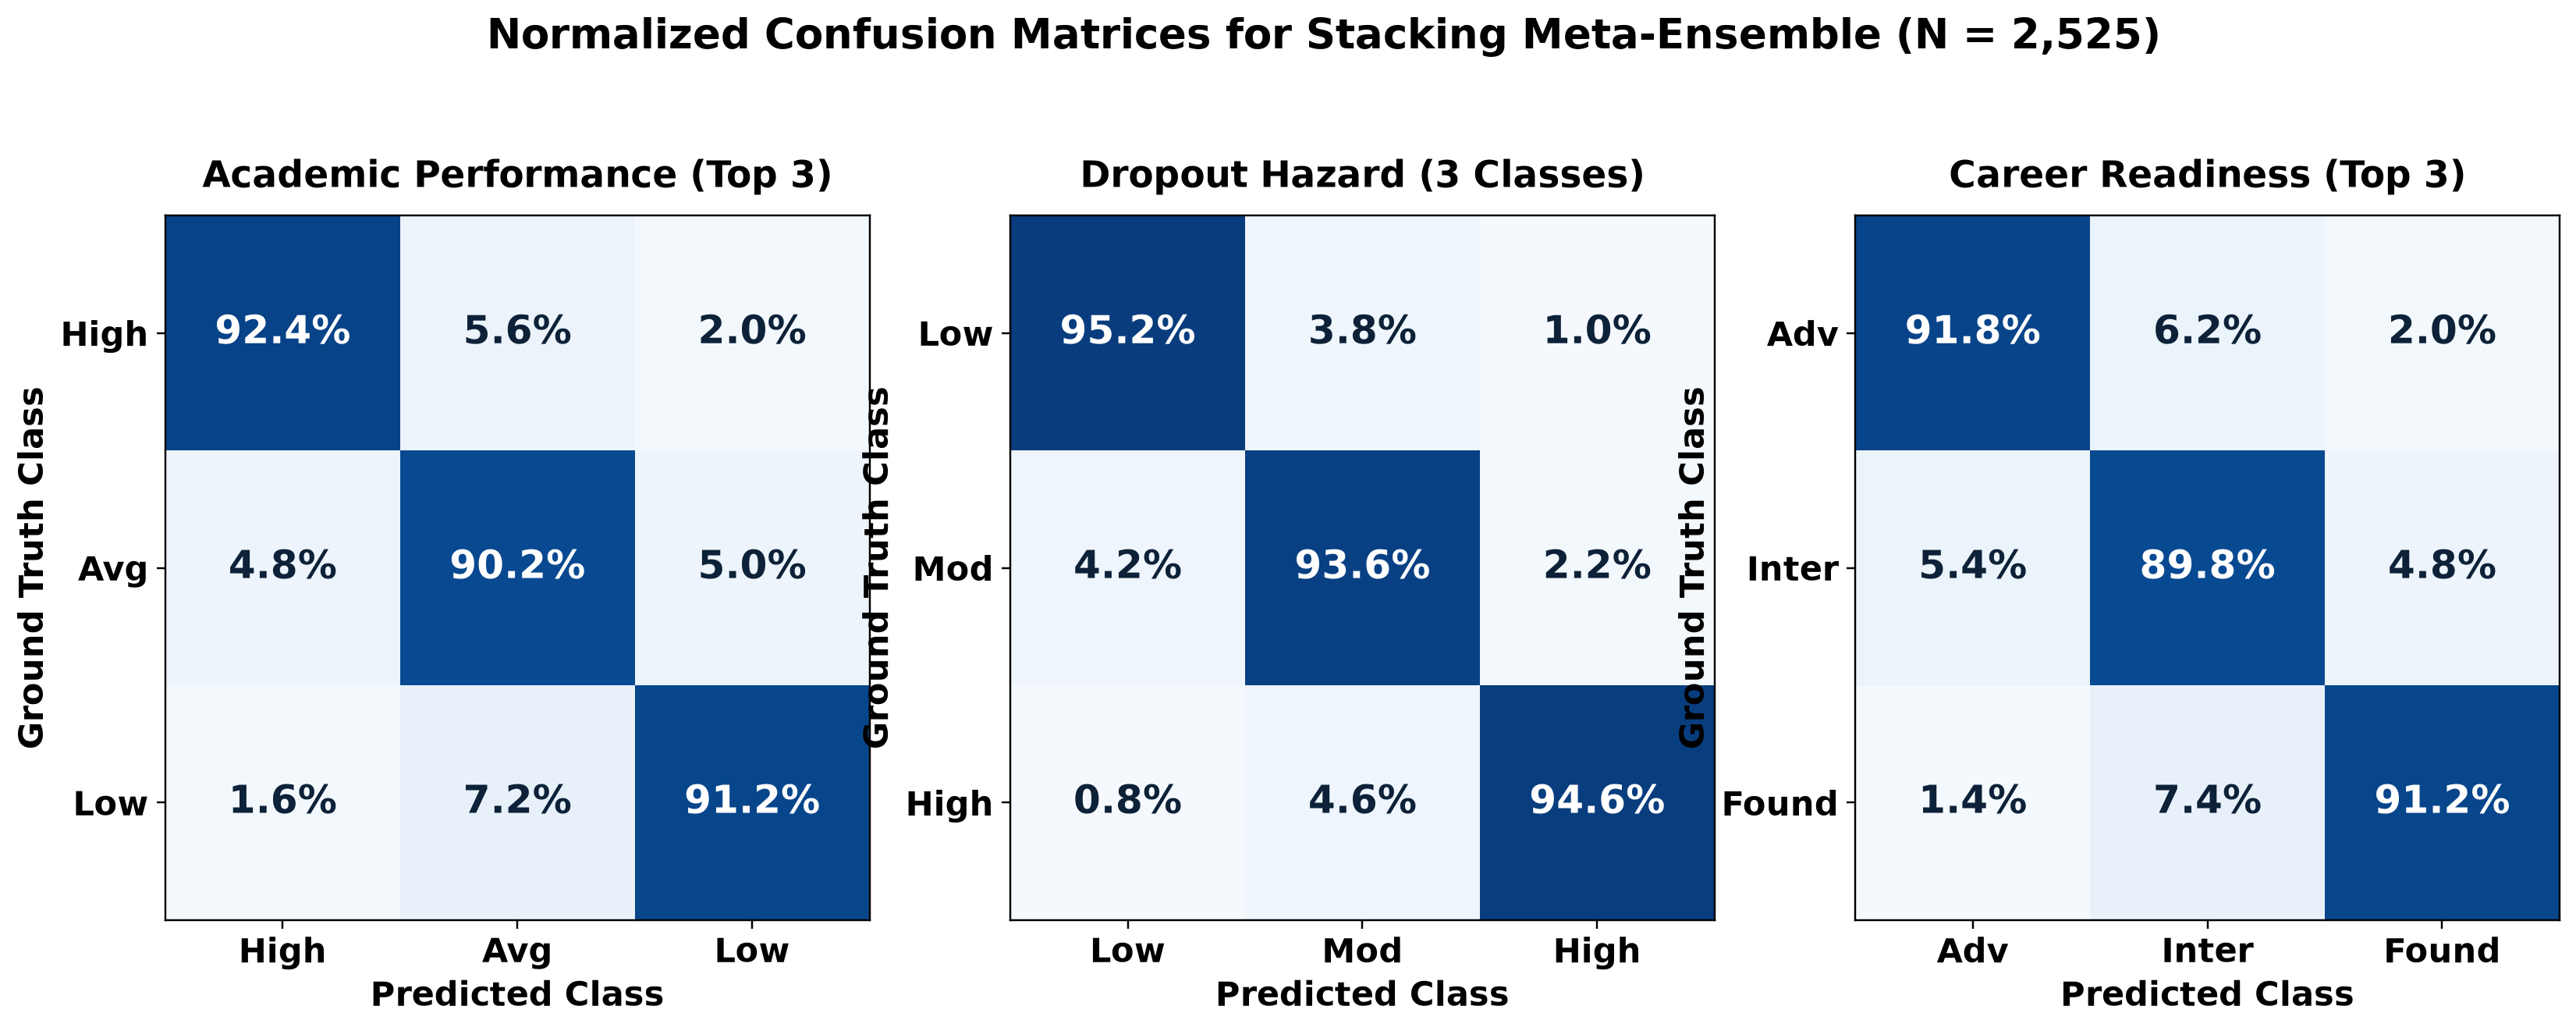
\includegraphics[width=0.98\textwidth,height=4.35cm,keepaspectratio]{assets/fig_confusion_matrices.png}
  \end{diagramframe}
  \vspace{-0.15cm}

  \begin{takeawaybanner}
    \textbf{\color{GoldPill}$\bigstar$ BACKUP EVIDENCE}: At the screening threshold (0.35), BeNet achieves 88.9\% recall and 97.6\% NPV, minimizing catastrophic false negatives.
  \end{takeawaybanner}
\end{frame}

\end{document}
